%% This is file `elsarticle-template-1-num.tex',
%%
%% Copyright 2009 Elsevier Ltd
%%
%% This file is part of the 'Elsarticle Bundle'.
%% ---------------------------------------------
%%
%% It may be distributed under the conditions of the LaTeX Project Public
%% License, either version 1.2 of this license or (at your option) any
%% later version.  The latest version of this license is in
%%    http://www.latex-project.org/lppl.txt
%% and version 1.2 or later is part of all distributions of LaTeX
%% version 1999/12/01 or later.
%%
%% The list of all files belonging to the 'Elsarticle Bundle' is
%% given in the file `manifest.txt'.
%%
%% Template article for Elsevier's document class `elsarticle'
%% with numbered style bibliographic references
%%
%% $Id: elsarticle-template-1-num.tex 149 2009-10-08 05:01:15Z rishi $
%% $URL: http://lenova.river-valley.com/svn/elsbst/trunk/elsarticle-template-1-num.tex $
%%
%%\documentclass[preprint,12pt]{elsarticle}

%% Use the option review to obtain double line spacing
%% \documentclass[preprint,review,12pt]{elsarticle}

%% Use the options 1p,twocolumn; 3p; 3p,twocolumn; 5p; or 5p,twocolumn
%% for a journal layout:
%% \documentclass[final,1p,times]{elsarticle}
%% \documentclass[final,1p,times,twocolumn]{elsarticle}
%% \documentclass[final,3p,times]{elsarticle}
 \documentclass[final,3p,times,twocolumn]{elsarticle}
%% \documentclass[final,5p,times]{elsarticle}
%% \documentclass[final,5p,times,twocolumn]{elsarticle}

%% if you use PostScript figures in your article
%% use the graphics package for simple commands
%% \usepackage{graphics}
%% or use the graphicx package for more complicated commands
%% \usepackage{graphicx}
%% or use the epsfig package if you prefer to use the old commands
%% \usepackage{epsfig}

%% The amssymb package provides various useful mathematical symbols
\usepackage{amssymb}
%% The amsthm package provides extended theorem environments
%% \usepackage{amsthm}

%% The lineno packages adds line numbers. Start line numbering with
%% \begin{linenumbers}, end it with \end{linenumbers}. Or switch it on
%% for the whole article with \linenumbers after \end{frontmatter}.
%% \usepackage{lineno}

%% natbib.sty is loaded by default. However, natbib options can be
%% provided with \biboptions{...} command. Following options are
%% valid:

%%   round  -  round parentheses are used (default)
%%   square -  square brackets are used   [option]
%%   curly  -  curly braces are used      {option}
%%   angle  -  angle brackets are used    <option>
%%   semicolon  -  multiple citations separated by semi-colon
%%   colon  - same as semicolon, an earlier confusion
%%   comma  -  separated by comma
%%   numbers-  selects numerical citations
%%   super  -  numerical citations as superscripts
%%   sort   -  sorts multiple citations according to order in ref. list
%%   sort&compress   -  like sort, but also compresses numerical citations
%%   compress - compresses without sorting
%%
%% \biboptions{comma,round}

% \biboptions{}

% HPS stuff
\usepackage{color}
%\usepackage{multicol}
\newcommand{\Aprime}{A\ensuremath{^\prime}}
\newcommand{\ee}{e$^+$e$^-$}
\newcommand{\fluenceunit}{1~MeV~neutron~equivalent/cm\ensuremath{^2}}
\newcommand{\geant}{{\sc Geant4}}
\newcommand{\egs}{{\sc EGS5}}
\newcommand{\moliere}{Moli\`{e}re}
%\include{affiliations}

\journal{Nuclear Physics B}

\begin{document}

\begin{frontmatter}

%% Title, authors and addresses

%% use the tnoteref command within \title for footnotes;
%% use the tnotetext command for the associated footnote;
%% use the fnref command within \author or \address for footnotes;
%% use the fntext command for the associated footnote;
%% use the corref command within \author for corresponding author footnotes;
%% use the cortext command for the associated footnote;
%% use the ead command for the email address,
%% and the form \ead[url] for the home page:
%%
%% \title{Title\tnoteref{label1}}
%% \tnotetext[label1]{}
%% \author{Name\corref{cor1}\fnref{label2}}
%% \ead{email address}
%% \ead[url]{home page}
%% \fntext[label2]{}
%% \cortext[cor1]{}
%% \address{Address\fnref{label3}}
%% \fntext[label3]{}

\title{The Heavy Photon Search Test Detector}


%%%%%%%%%%%%%%%%%%%%%%%%%%%%%%%%%%%%%%%%%%%%%%%%%%
%% use optional labels to link authors explicitly to addresses:
%% \author[label1,label2]{<author name>}
%% \address[label1]{<address>}
%% \address[label2]{<address>}


\newcommand{\red[1]}{{\color{red}{\bf #1}}}
\newcommand{\JLAB}{Thomas Jefferson National Accelerator Facility, Newport News, Virginia 23606}
\newcommand{\CUA}{Catholic University of America, Washington, D.C. 20064}
\newcommand{\OU}{Ohio University,  Athens, Ohio 45701}
\newcommand{\YEREVAN}{Yerevan Physics Institute, 375036 Yerevan, Armenia}
\newcommand{\SCAROLINA}{University of South Carolina, Columbia, South Carolina 29208}
\newcommand{\NSU}{Norfolk State University, Norfolk, Virginia 23504}
\newcommand{\ODU}{Old Dominion University, Norfolk, Virginia 23529}
\newcommand{\genova}{Istituto Nazionale di Fisica Nucleare, Sezione di Genova e Dipartimento di Fisica dell\'Universita, 16146 Genova, Italy}
\newcommand{\SACLAY}{CEA, Centre de Saclay, Irfu/Service de Physique Nucl\'eaire 91191 Gif-sur-Yvette, France}
\newcommand{\ORSAY}{Institut de Physique Nucleaire d'Orsay, IN2P3, BP 1, 91406 Orsay, France}
\newcommand{\ECOLE}{CPhT, Ecole Polytechnique, F 91128 PALAISEAU CEDEX, France}
\newcommand{\UCSC}{University of California, Santa Cruz, CA 95064}
\newcommand{\SUNY}{Stony Brook University, Stony Brook, NY 11794-3800}
\newcommand{\FNAL}{Fermi National Accelerator Laboratory, Batavia, IL 60510-5011}
\newcommand{\UNH}{University of New Hampshire, Department of Physics, Durham, NH 03824}
\newcommand{\PERIMETER}{Perimeter Institute, Ontario, Canada N2L 2Y5}
\newcommand{\RPI}{Rensselaer Polytechnic Institute, Department of Physics, Troy, NY 12181}
\newcommand{\SLAC}{SLAC National Accelerator Laboratory, Menlo Park, CA 94025}
\newcommand{\WNM}{The College of William and Mary, Department of Physics, Williamsburg, VA 23185}


\author[SLAC]{C. Field}
\author[SLAC]{P. Hansson Adrian\corref{corrauthor}}
\author[SLAC]{N. Graf} 
\author[SLAC]{ M. Graham} 
\author[SLAC]{ G. Haller} 
\author[SLAC]{ R. Herbst} 
%\author[SLAC]{ J. Jaros\corref{spoks}} 
\author[SLAC]{ J. Jaros}
\author[SLAC]{T. Maruyama} 
\author[SLAC]{ J. McCormick} 
\author[SLAC]{ K. Moffeit} 
\author[SLAC]{ T. Nelson} 
\author[SLAC]{ H. Neal} 
\author[SLAC]{ A. Odian} 
\author[SLAC]{ M. Oriunno} 
\author[SLAC]{ S. Uemura} 
\author[SLAC]{ D. Walz}
%
\author[UCSC]{A. Grillo} 
\author[UCSC]{ V. Fadeyev} 
\author[UCSC]{ O. Moreno}
%
\author[FNAL]{W. Cooper}
%
\author[JLAB]{S. Boyarinov} 
\author[JLAB]{ V. Burkert} 
\author[JLAB]{ A. Deur} 
\author[JLAB]{ H. Egiyan}
 \author[JLAB]{ L. Elouadrhiri} 
 \author[JLAB]{ A. Freyberger} 
 \author[JLAB]{ F.-X. Girod} 
 \author[JLAB]{ V. Kubarovsky} 
\author[JLAB]{ Y. Sharabian} 
%\author[JLAB]{ S. Stepanyan\corref{spoks}} 
\author[JLAB]{ S. Stepanyan}
\author[JLAB]{ M. Ungaro} 
\author[JLAB]{ B. Wojtsekhowski}
%
\author[SUNY]{R. Essig}
%
%\author[UNH]{M. Holtrop\corref{spoks}} 
\author[UNH]{M. Holtrop}
\author[UNH]{ K. Slifer} 
\author[UNH]{ S. K. Phillips}
%
\author[ORSAY]{A. Fradi} 
\author[ORSAY]{ B. Guegan} 
\author[ORSAY]{ M. Guidal} 
\author[ORSAY]{ S. Niccolai} 
\author[ORSAY]{ S. Pisano} 
\author[ORSAY]{ E. Rauly}
\author[ORSAY]{ P. Rosier}
\author[ORSAY]{D. Sokhan}
 %
\author[PERIMETER]{P. Schuster} 
\author[PERIMETER]{ N. Toro}
%
\author[YEREVAN]{N. Dashyan} 
\author[YEREVAN]{ N. Gevorgyan} 
\author[YEREVAN]{ R. Paremuzyan}
\author[YEREVAN]{ H. Voskanyan}
%
\author[NSU]{M. Khandaker} 
\author[NSU]{ C. Salgado}
%
\author[GENOVA]{M. Battaglieri} 
\author[GENOVA]{ R. De Vita}
%
\author[ODU]{S. Bueltmann} 
\author[ODU]{ L. Weinstein}
%
\author[RPI]{P. Stoler} 
\author[RPI]{A. Kubarovsky}
%
\author[WNM]{K. Griffioen}

\address[SLAC]{\SLAC}                                 
\address[UCSC]{\UCSC}
\address[FNAL]{\FNAL}
\address[JLAB]{\JLAB}
\address[SUNY]{\SUNY}
\address[UNH]{\UNH}
\address[ORSAY]{\ORSAY}
\address[PERIMETER]{\PERIMETER}
\address[YEREVAN]{\YEREVAN}
\address[NSU]{\NSU}
\address[GENOVA]{\genova}
\address[ODU]{\ODU}
\address[RPI]{\RPI}
\address[WNM]{\WNM}

 %\cortext[spoks]{Co-spokesperson}

\cortext[corrauthor]{Corresponding author. \ead{phansson@slac.stanford.edu}}





%\author[label1]{Per Ledin}
%\ead{contact@hps.discovery.com}
%\author[slac]{Per Hansson Adrian\corref{cor1}}
%\ead{phansson@slac.stanford.edu}
%\author[slac]{Timothy K. Nelson}
%\address[slac]{SLAC National Accelerator Laboratory, 94025, Menlo Park, CA, USA}
%\address[label1]{Lule\aa~Hockey}

%%%%%%%%%%%%%%%%%%%%%%%%%%%%%%%%%%%%%%%%%%%%%%%%%%



\begin{abstract}
The  Heavy Photon Search (HPS), an experiment to search for a hidden sector photon in fixed target 
electroproduction, is preparing for installation at the Thomas Jefferson National Accelerator Facility 
(JLab) in the Fall of 2014.  As the first stage of this project, the HPS Test run apparatus was 
constructed and operated in 2012 to demonstrate the experiment's technical feasibility and to  confirm 
that the trigger rates and occupancies are as expected. This paper describes the Test Run apparatus 
and readout electronics and its performance. In this setting, a heavy photon can be identified as a 
narrow\ee  mass peak above the trident background or as a decay vertex displaced from
the production target, so charged particle tracking and vertexing are needed for its detection. In the 
HPS Test run, charged particles are measured
with a compact forward silicon microstrip vertex/tracker inside a dipole magnet. Electromagnetic 
showers are detected in a PbW0$_{4}$ 
crystal calorimeter situated behind the magnet used to trigger the experiment and identify 
electrons and positrons. Both detectors are placed close to the 
beam line and split top-bottom. This arrangement  provides sensitivity to low-mass heavy photons,  
allows clear  passage of the unscattered beam, 
and avoids the spray of degraded electrons coming from the target. 
The discrimination between prompt and displaced \ee pairs requires the first layer of silicon 
sensors be placed only 10~cm downstream of the target. The expected signal is small, and the 
trident background huge, so the experiment requires very large statistics. Accordingly, the
HPS Test run utilizes  high-rate readout and data acquisition electronics and a fast trigger to
perfectly exploit the essentially 100\% duty cycle of the CEBAF accelerator.
\end{abstract}

\begin{keyword}
%% keywords here, in the form: keyword \sep keyword
silicon microstrip \sep tracking  \sep vertexing \sep heavy photon \sep dark photon \sep hidden sector \sep electromagnetic calorimeter
%% MSC codes here, in the form: \MSC code \sep code
%% or \MSC[2008] code \sep code (2000 is the default)

\end{keyword}

\end{frontmatter}

\clearpage
\tableofcontents
\clearpage
\newpage
\newpage

%%
%% Start line numbering here if you want
%%
% \linenumbers

%% main text
\section{Introduction}
\label{introduction}
The heavy photon (\Aprime{}), aka a "hidden sector" or "dark" photon, is a particle with mass 
$10-1000$~MeV which couples weakly to electric charge by mixing with the Standard Model 
photon~\cite{Holdom:1985ag}. Consequently, it can be radiated by electrons and subsequently decay 
into \ee pairs, albeit at rates far below those of QED trident processes. Heavy photons have been 
suggested by numerous Beyond Standard Model theories `\cite{Essig:2013lka}, to explain the 
discrepancy 
between theory and experiment of the muon's $g-2$ ~\cite{Pospelov:2008zw}, and as a possible 
explanation of recent astrophysical anomalies.  Heavy photons  couple directly to  hidden sector 
particles with "dark" or "hidden sector" charge; these particles
could constitute all or some of the dark matter~\cite{ArkaniHamed:2008qn}. 
Current phenomenology highlights the $20-1000$~MeV/c$^{2}$ mass range, and 
suggests that  the coupling to electric charge, $\epsilon$e, has $\epsilon$ in the range of 
$10^{-3} -10^{-5}$. [REFERENCE]. This range of parameters makes \Aprime{} searches viable in 
medium energy fixed target electroproduction~\cite{Bjorken:2009mm}, but requires large data sets and 
good mass resolution to identify a small mass peak above the copious QED background. At small 
couplings, \Aprime's become long-lived, so detection of a displaced decay vertex can reject the prompt 
QED background and boost experimental sensitivity.  

The HPS experiment~\cite{HPS_proposal_2010} uses both invariant mass and secondary
vertex signatures to search for A's. It uses  a $\approx 1$~m long silicon tracking and vertexing detector
inside a dipole magnet to measure charged particle trajectories and a fast electromagnetic calorimeter 
just downstream of the magnet to provide a trigger and identify electrons. The experiment utilizes very 
high rate front end electronics and runs at high trigger rates (up to 50kHz), exploiting the 100\% duty 
cycle of the Thomas Jefferson National Accelerator Facility (JLab) CEBAF accelerator to accumulate 
the needed statistics. 

The HPS Test apparatus, a simplified version of the HPS experiment, was proposed and 
approved at Thomas Jefferson National Accelerator Facility (JLab) as the first stage of HPS. 
Its purposes included demonstrating that the apparatus and data acquisition systems are 
technically feasible and  the trigger rates and occupancies to be  encountered in electron-beam 
running are as simulated. Given dedicated running time with electron beams, the HPS Test Run 
apparatus is capable of searching for heavy photons in unexplored regions of parameter space.    
The key design criteria for HPS and the HPS Test Run are the same:
\begin{itemize}
\item large and uniform acceptance in the forward region close to the beam in order to catch boosted 
\Aprime{} decay products,
\item beam passage through the apparatus in vacuum, to eliminate direct interactions with the 
detector and minimize beam gas interactions, 
\item a flexible, redundant and efficient trigger selecting electron and positron pairs at rates up to 
50~kHz,
\item excellent track reconstruction efficiency for electrons and positrons,
\item good angular and momentum resolution to reconstruct invariant mass precisely,
\item excellent vertex resolution to discriminate displaced \Aprime{} decays from prompt QED 
backgrounds,
\item high rate electronics with excellent timing resolution to minimize out of time backgrounds,
\item data handling rates of 100~MB/s to permanent storage,
\item detector components that can survive and efficiently operate in a high radiation environment 
with local doses exceeding $100$~Mrad.
\end{itemize}


The Test apparatus was installed on April 19, 2012, and ran parasitically in the photon beam of the HDice 
experiment~\cite{HDice} until May 18. The JLab run schedule 
precluded any dedicated electron beam running, but the HPS Test Run was allowed a short and 
valuable dedicated run at the end of scheduled CEBAF running. This final running provided
enough data to demonstrate the functionality of the apparatus, document its performance, and
explore trigger rates, as shown below. 
This paper reviews the HPS Test apparatus; documents the performance of the trigger, 
data acquisition, silicon tracking detector, and the electromagnetic calorimeter at the level assumed 
in calculating the physics reach of the HPS experiment. 



This paper reviews the HPS Test apparatus; documents the performance of the trigger, 
data acquisition, silicon tracking detector, and the electromagnetic calorimeter at the level assumed 
in calculating the physics reach of the HPS experiment. 



\section{Detector Overview}
\label{detector}
{\small
\begin{figure*}[t]
\begin{center}
    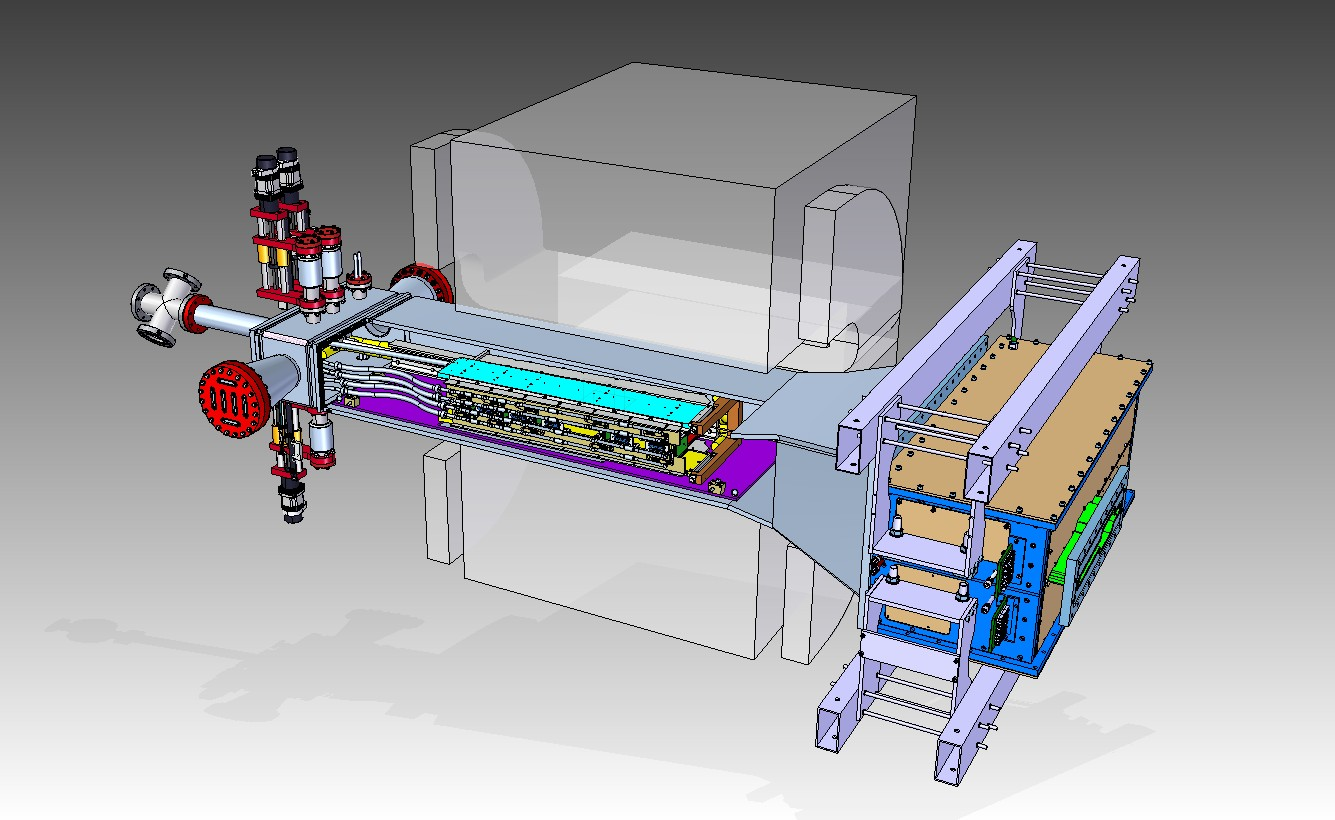
\includegraphics[width=0.8\textwidth]{figures/hps_testrun_rendering}
\caption{Rendering of the HPS Test apparatus installed on the beam line.}
\label{fig:testrundetector}
\end{center}
\end{figure*}
}
The HPS Test apparatus was designed to run in Hall~B at JLab using the CEBAF electron beam, a 
499~MHz beam, at an energies of 2.2 and 6.6~GeV and currents between 200 and 600~nA.  
The overall design of the experiment follows from the kinematics of \Aprime{} production which 
typically results in a final state particle within a few degrees of the incoming beam, especially at low 
$m_{\textrm{A}^\prime}$. Detectors must therefore be placed close to the beam. 
The intense electron beam enlarges downstream after multiple scattering in the target and electrons 
which have radiated in the target disperse horizontally in the field of the analyzing magnet. Together 
they constitute a "wall of flame" which must be completely avoided. Accordingly, 
the apparatus is split vertically to avoid a "dead zone", the region within $\pm 15$~mrad of the beam 
plane. In addition, the beam is transported in vacuum through the tracker to minimize beam-gas 
interaction backgrounds. Even with these precautions, the occupancies of sensors near the beam 
plane are high, dominated by the
multiple Coulomb scattering of the primary beam, so high rate detectors, a fast trigger, 
and excellent time tagging are required to minimize their impact.  
The trigger comes from a highly-segmented  PbWO$_{4}$ crystal calorimeter located just downstream 
of the dipole magnet. 
 %\begin{multicols}{2}
\begin{center}
\begin{table*}[t]
{\small
\caption{Overview of the coverage, segmentation and performance of the HPS Test detector. }
\begin{tabular}{lccccccc}
\hline 
System & Coverage & \# channels & ADC & Time resolution & \# layers & Segmentation & Performance \\
 & (mrad) &  & (bit) & (ns) &  &  &  \\
\hline
SVT & $15<\theta_{y} < XXXX$ & 12800 & 14 & $\approx 2$~ns & 5  & $\approx 120~\mu$m $r-\phi$ & $\sigma_{d0,y}  \approx 100~\mu$m \\
& &  &  &  & (stereo layers) & $\approx 6~\mu$m $z$ & $\sigma_{d0,x} \approx 300~\mu$m \\
& &  &  &  &  &  & $\sigma_{d0,z}\approx 1$~mm \\
\hline
ECal & $15<\theta_{y} < XXXX$ & 442 & 12 & 4~ns & 1 & $1.3\times1.3$~cm$^2$  & $\sigma(E)/E \approx 4.5\%$ \\ 
 &  &  &  &  &  & $1.6\times1.6$~cm$^2$  &  \\ 
\hline
\end{tabular}
\label{tab:detector-overview}
}
\end{table*}
\end{center}
%\end{multicols}
A rendering of the apparatus installed on the beam line is shown in 
Fig.~\ref{fig:testrundetector} and an overview of the coverage, segmentation and performance is 
given in Tab.~\ref{tab:detector-overview}.  

The silicon tracking and vertexing detector for HPS Test, or SVT, resides in a vacuum 
chamber inside the pair spectrometer analyzing magnet in Hall B at JLab. The SVT has five 
measurement stations, or ``layers,'' beginning10 cm downstream of the target. Each layer 
comprises a pair of closely-spaced silicon microstrip sensors responsible for measuring a single 
coordinate, or ``view.'' Introduction of a small (50 or 100~mrad) stereo angle between the two 
sensors of each layer provides three-dimensional tracking and vertexing throughout the acceptance 
of the detecto. In order to accommodate the dead zone, the 
SVT is built in two halves that are approximately mirror reflections of one another about the plane of the 
nominal electron beam.  Each layer in one half is supported on a common support plate with 
independent cooling and readout. 

The electomagnetic calorimeter (ECal) is also split into two halves. Each half of the ECal consists of 
221 PbWO$_4$ crystals arranged in rectangular formation. There are five rows with 46 modules in 
each row except the row closest to the beam plane which has 37. The light from each crystal 
is read out by an Avalanche Photodiode (APD) glued on the back surface of the crystal. 
Signals from the APDs are amplified using custom-made amplifier boards before being sent to the 
data acquisition electronics.

The  Data Acquisition system combines two architectures, the Advanced Telecom Communications 
Architecture (ATCA) based SVT readout system and VMEbus Switched Serial (VXS) based digitization 
and triggering system for the ECal. The system was designed to run at up to 20~kHz trigger rate.



%%%%%%%%%%%%%%%%%%%%%%%%%%%%%%%%%%%%%%%%%%%%%%%%%%


\section{The HPS Test Run Beamline}
The HPS Test run studied multiple Coulomb scattering of electrons and positrons from 
bremsstrahlung photons produced in the Hall B tagged photon facility. 
Figure~\ref{fig:hpstest_layout} shows the layout of 
the setup on the beam line. The SVT was installed inside the Hall B pair 
spectrometer magnet (PS) vacuum chamber with the ECal mounted downstream of it. Both the 
SVT and the ECal were retracted off the beam plane compared to nominal electron beam runing to 
allow clean passage of the photon beam through the system. 
\begin{figure}[]
    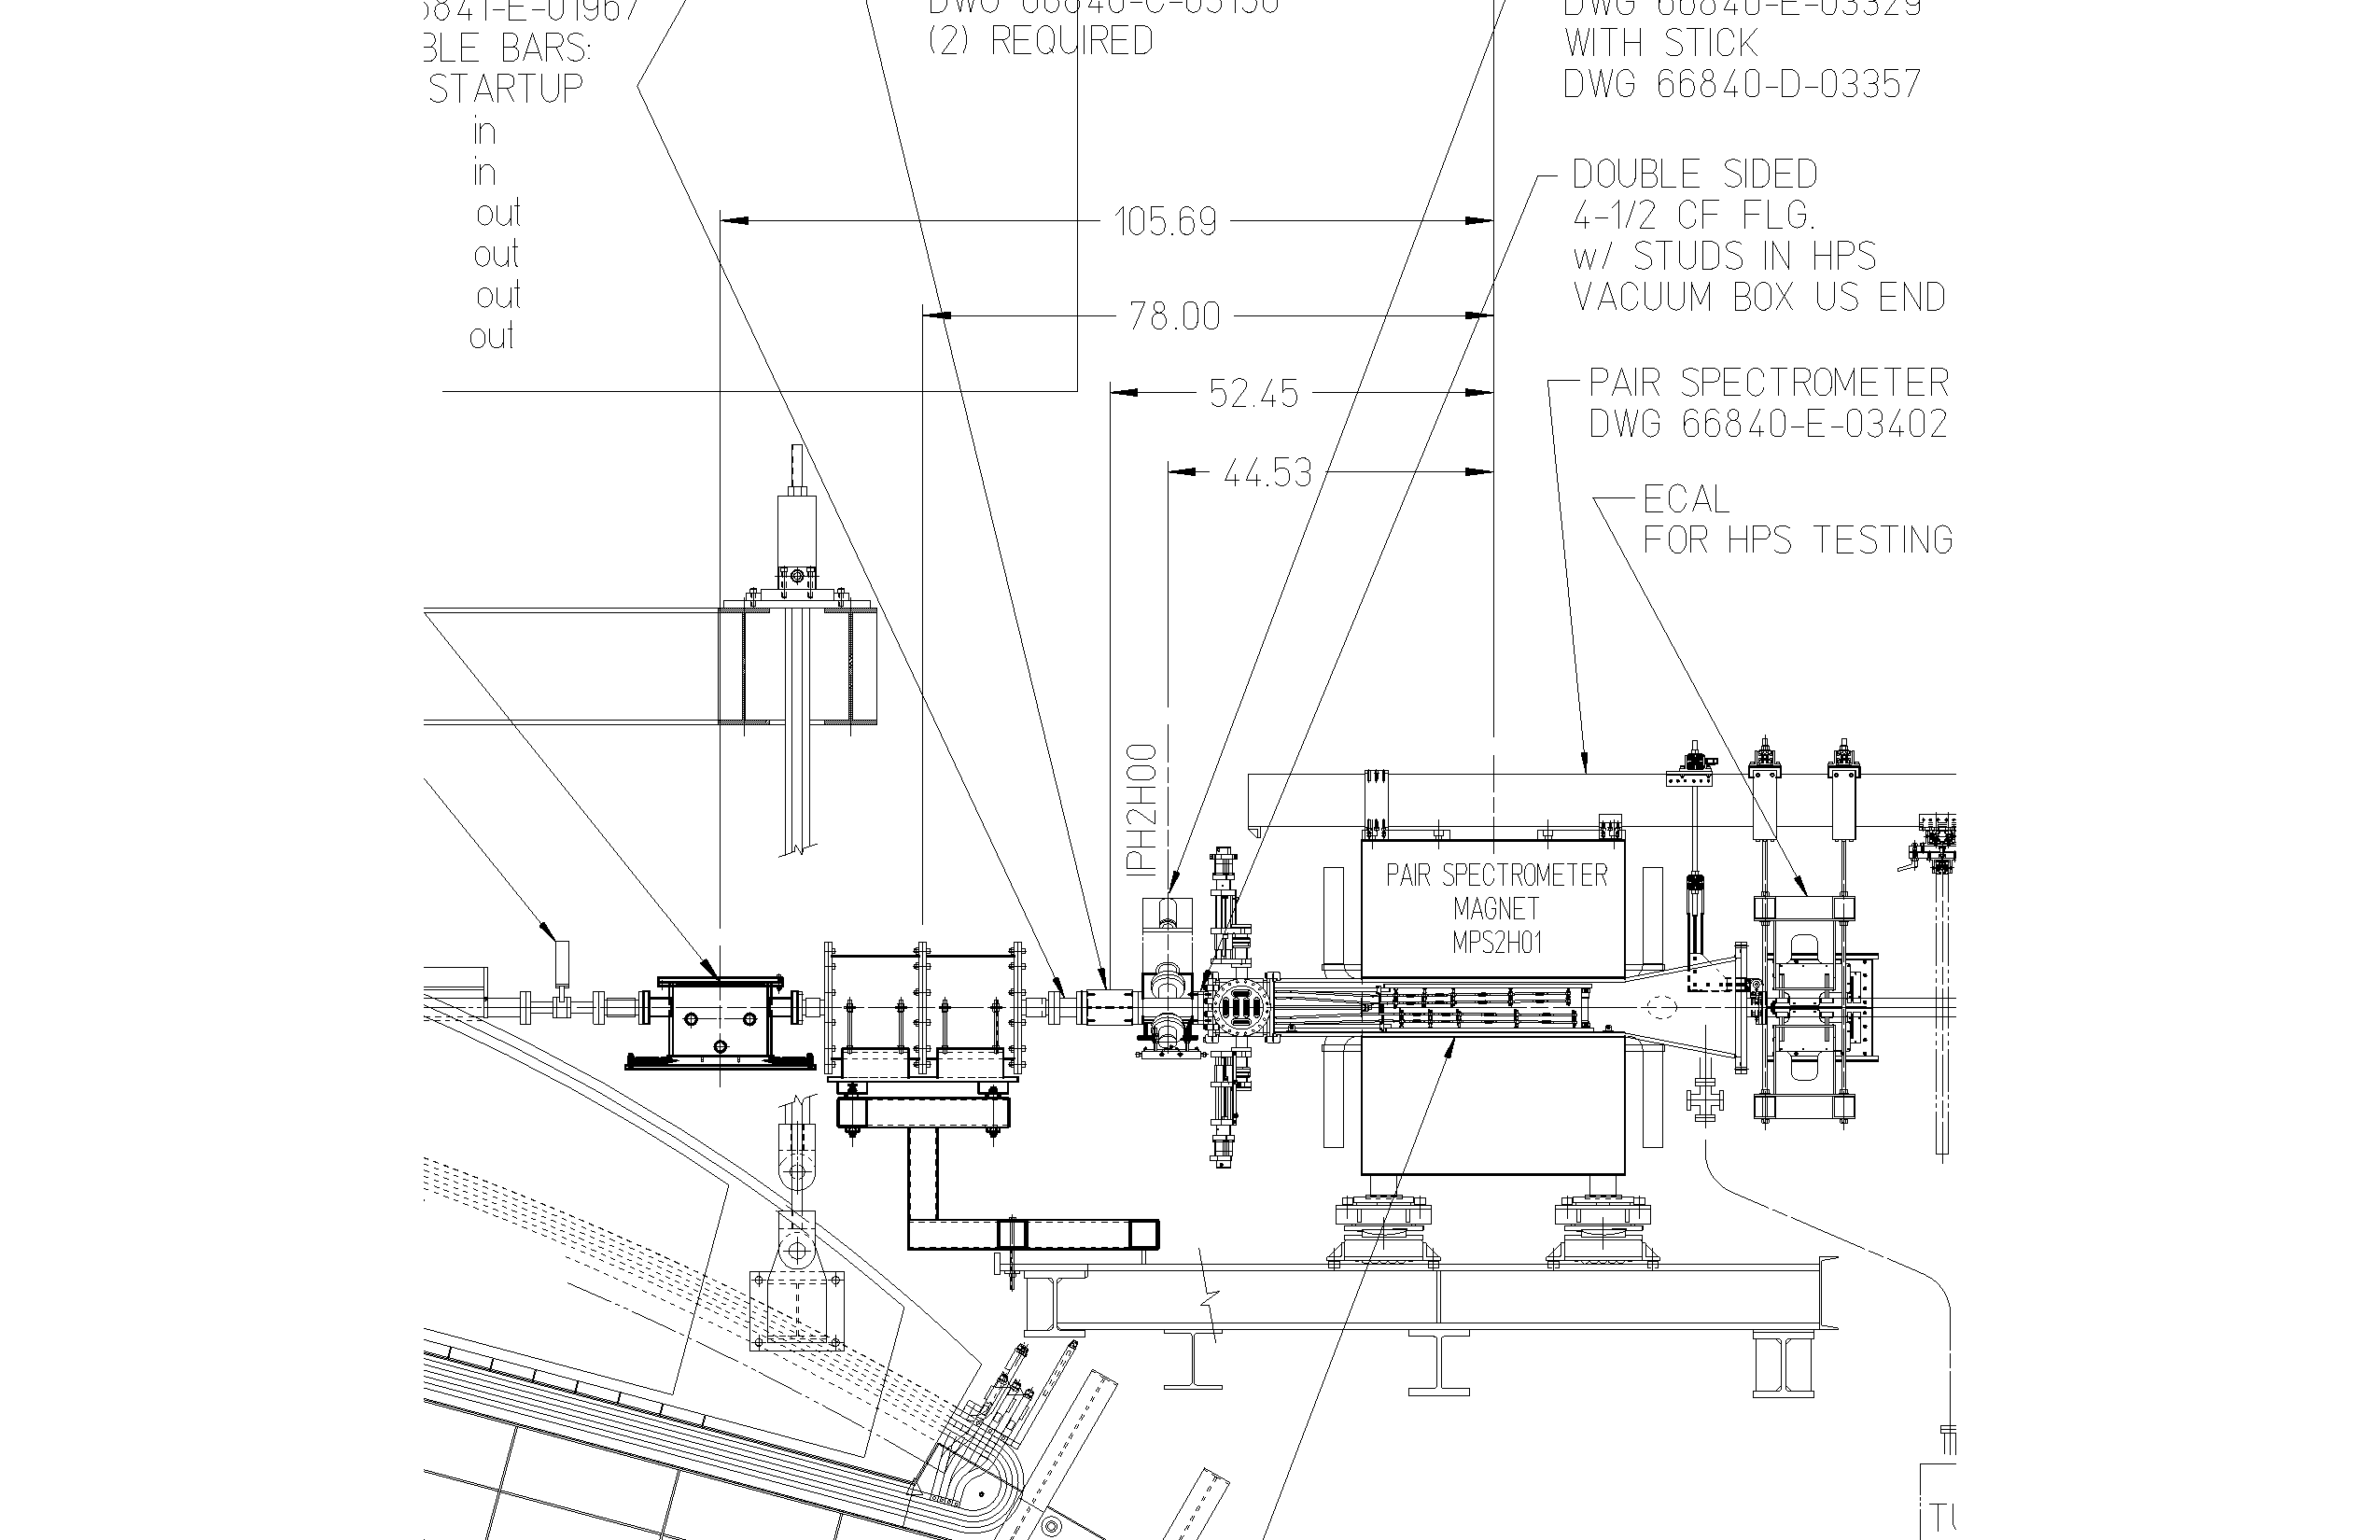
\includegraphics[width=0.5\textwidth]{figures/HPS_dimensions}
\caption{\small{Layout of the HPS parasitic run.} }
\label{fig:hpstest_layout}
\end{figure}

The photon beam was generated in the interaction of $5.5$~GeV electrons with a $10^{-4}~X_0$ 
gold radiator located $\approx~9$~m upstream of the PS. The primary beam and scattered 
electrons are deflected away from detectors by the dipole magnet of the photon tagging system. 
During the dedicated HPS Test run period, the collimated (6.4~mm diameter), photon beam passes 
through the aluminum PS pair converter and later the HPS system as illustrated in 
Fig.~\ref{fig:schematic_testrun_vs_erun}.
\begin{figure}[]
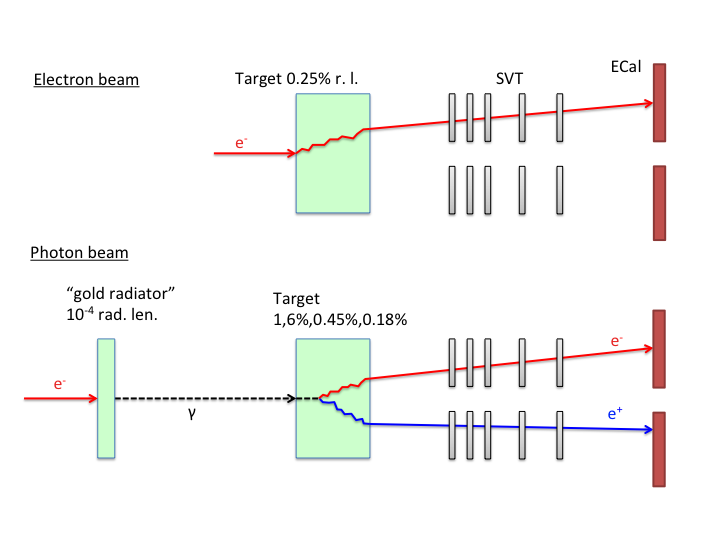
\includegraphics[ width=7cm]{figures/photon_vs_electron_beam_schematic.png}
\caption{\small{Illustrative comparison of HPS Test run photon beam compared to the HPS electron 
beam.}}
\label{fig:schematic_testrun_vs_erun}
\end{figure}
The PS pair converter was located $\approx~77$~cm upstream of the first layer of the SVT.
 
 
 Data was taken on three different converter thicknesses with photon fluxes between 
 1.1-2.6$\times10^{8}$/s ($0.55<$E$_\gamma<5.5$~GeV) at beam currents varying between 
 30-90~nA and repeated with the reverse field setting of the PS dipole magnet.
\begin{table}[]
\begin{center}
{\small
\begin{tabular}{|c|c|c|}
\hline
Converter thickn. & Duration &  $e^-$ on radiator \\
 (\%$X_0$) & (s) & ($\mu$C)    \\   
\hline
%\hline
1.6   & 911 &   24.4 \\ %24385.9     \\ %27 nA
%\hline
0.18   & 2640 &   193.5 \\ % 193508.9  \\  %73 nA
%\hline
0.45  & 2149 &     140.7 \\ %  140709.9  \\ %65.5 nA
%\hline
0    & 1279  &   88.1 \\ %88079.6  \\
\hline
\end{tabular}
}
\caption{Measured integrated currents for the dedicated photon runs.}
\label{tab:currents}
\end{center}
\end{table}
The photon beam line during the test run produced a relatively large fraction of pairs 
originating upstream of the converter position. This contribution was measured during data taking 
with ``empty'' converter runs i.e. removing the converter but with all other conditions the same. 
The runs taken during the time dedicated to HPS Test is summarized in Tab.~\ref{tab:currents}.



%%%%%%%%%%%%%%%%%%%%%%%%%%%%%%%%%%%%%%%%%%%%%%%%%%

\section{Silicon Vertex Tracker}
\label{svt}

The Silicon Vertex Tracker (SVT) enables efficient reconstruction of charged particles and precision 
determination of their trajectories. These measurements allow \Aprime{} decays to be distinguished 
from background via simultaneous estimation of the invariant mass of \ee{} decay products and the 
position of decay vertexes downstream of the target. 

The design of the SVT is primarily driven by direct physics requirements and constraints from the 
environment at the interaction region. The \Aprime decay products 
have momenta in the range of 1~GeV, so multiple scattering dominates mass and vertexing 
uncertainties for any possible material budget, so the SVT must minimize the amount of 
material in the tracking volume. The signal yield for long-lived \Aprime's is very small, so 
the rejection of prompt vertexes must be exceedingly pure, on the order of $10^{-7}$, in order to 
eliminate all prompt backgrounds. To achieve the required vertexing performance the first layer of the 
SVT must be placed no more than about 10 cm downstream of the target. At that distance, it is found 
that the active region of a sensor can be placed as close to 1.5 mm from the center of the beam, 
defining the 15 mrad ``dead zone" mentioned previously, to maximize low-mass \Aprime acceptance 
with decay products nearly collinear with the beam axis. At the edge of this ``dead zone," the 
radiation dose approaches $10^{15}$ electrons/cm$^2$/month, or roughly 
$3 \times 10^{14}$~\fluenceunit{}/month~\cite{Rashevskaya:2002nd}, 
requiring the sensors to be actively cooled.
% and~\ref{fig:rates}.
%===================
%\begin{figure}[]
%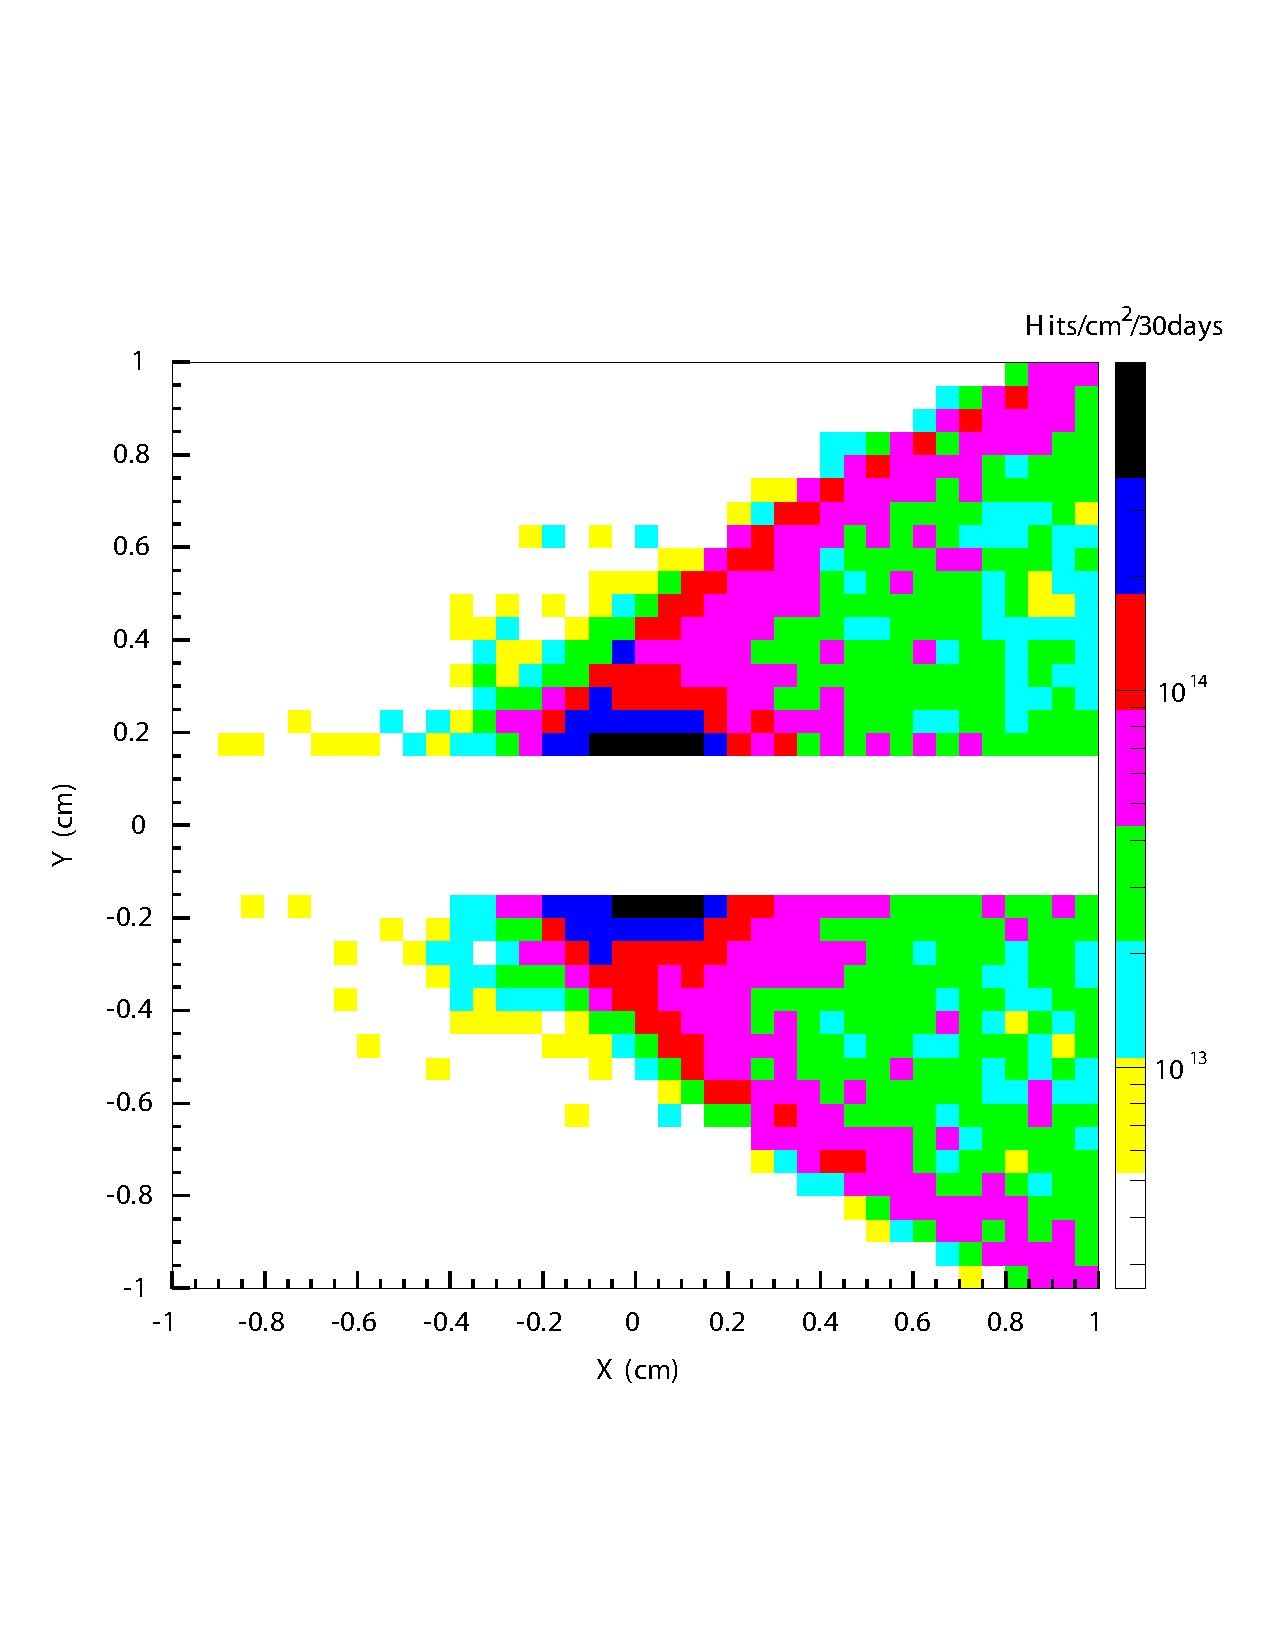
\includegraphics[width=7cm]{figures/radiation}
%\label{fig:radiation}
%\caption{{\small Simulation of the electron fluence 10~cm downstream of the target in the active region 
%of the SVT ($|Y|>0.15~$mm) looking downstream; electrons bend towards $+x$.}}
%\end{figure}
Meanwhile, very low-energy delta rays from 
beam-gas interactions multiply the density of background hits, so the SVT must operate inside the 
beam vacuum.  Finally, in order to protect the sensors, the detector must be movable so that it can be 
retracted during periods of uncertain beam conditions.  



\subsection{Layout}
The layout of the SVT is summarized in Tab.~\ref{tab:trk} and rendered in Fig.~\ref{fig:tracker_model}. 
Each of the layers is comprised of a pair of closely-spaced silicon microstrip sensors mounted back-
to-back to form a module. A 100~mrad stereo angle is used in the first three layers to provide higher-
resolution 3D space points for vertexing.  Using 50~mrad in the last two layers breaks the tracking 
degeneracy of having five identical layers and minimizes fakes from ghost hits to improve pattern 
recognition. Altogether, the SVTcomprises 20 sensors for a total of 12780 readout channels. 
%=======================
\begin{center}
\begin{table}[ht]
{\footnotesize
\begin{tabular}{lccccc}   
\hline \hline 
    Layer & 1 & 2 & 3 & 4 & 5 \\      
\hline
    $z$ from target (cm)  & 10 & 20 & 30 & 50 & 70  \\ 
    Stereo angle (mrad)  & 100 & 100 & 100 & 50 & 50 \\ 
    Bend res. ($\mu$m)  & $\approx$60 & $\approx$60 & $\approx$60 & $\approx$120 & $\approx$120  \\ 
    Non-bend res. ($\mu$m)  & $\approx$6 & $\approx$6 & $\approx$6 & $\approx$6 & $\approx$6  \\ 
    \# of sensors  & 4 & 4 & 4 & 4 & 4  \\ 
    Dead zone (mm) & $\pm1.5$  & $\pm3.0$  & $\pm4.5$  & $\pm7.5$  & $\pm10.5$  \\ 
    Power cons. (W) & 6.9 & 6.9 & 6.9 & 6.9 & 6.9 \\
\hline \hline
\end{tabular}
\caption{\small Layout of the SVT.}
}
\label{tab:trk}
\vspace*{-15mm}
\end{table}
\end{center}
%=======================
\begin{center}
\begin{figure}[htp]
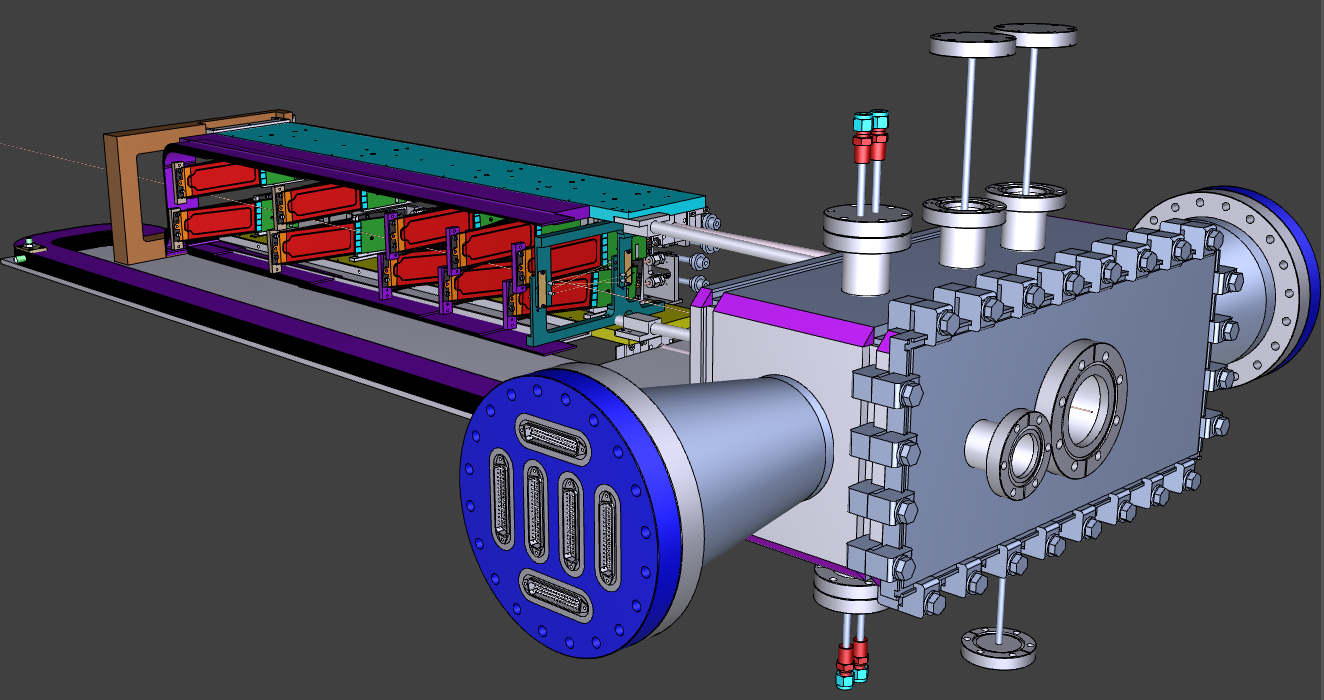
\includegraphics[width=7cm]{figures/HPS_nochamber}
\caption{\small A rendering of the SVT showing the modules on their support plates held by the 
hinged C-support on the left and the motion levers on the right. The sensors are shown in red and the 
hybrid readout boards in green. The beam enters from the right through a vacuum box with flanges 
for services. }
\label{fig:tracker_model}
%\vspace*{-5mm}
\end{figure}
\end{center}
%=======================
The SVT is built in two separate halves that are mirror reflections of one another about the plane of 
the nominal electron beam.  Each half consists of five modules mounted on a support plate that 
provides services to the modules and allows them to be moved as a group relative to the dead zone. 
The two halves of the tracker are connected to hinges mounted on a C-shaped support just beyond 
the last layer that defines the nominal spacing between the upper and lower halves of the tracker.  A 
shaft attached to each support plate in front of layer 1 extends upstream and connects to a linear shift 
that transfers motion into the vacuum box through bellows to open and close the two halves around 
the dead zone. The C-support is mounted to an aluminum baseplate that defines the position of the 
SVT with respect to the vacuum chamber. Figure~\ref{fig:tracker_halves} shows a photograph of both 
completed detector halves prior to final assembly. 
%=======================
\begin{figure}[htp]
\begin{center}
    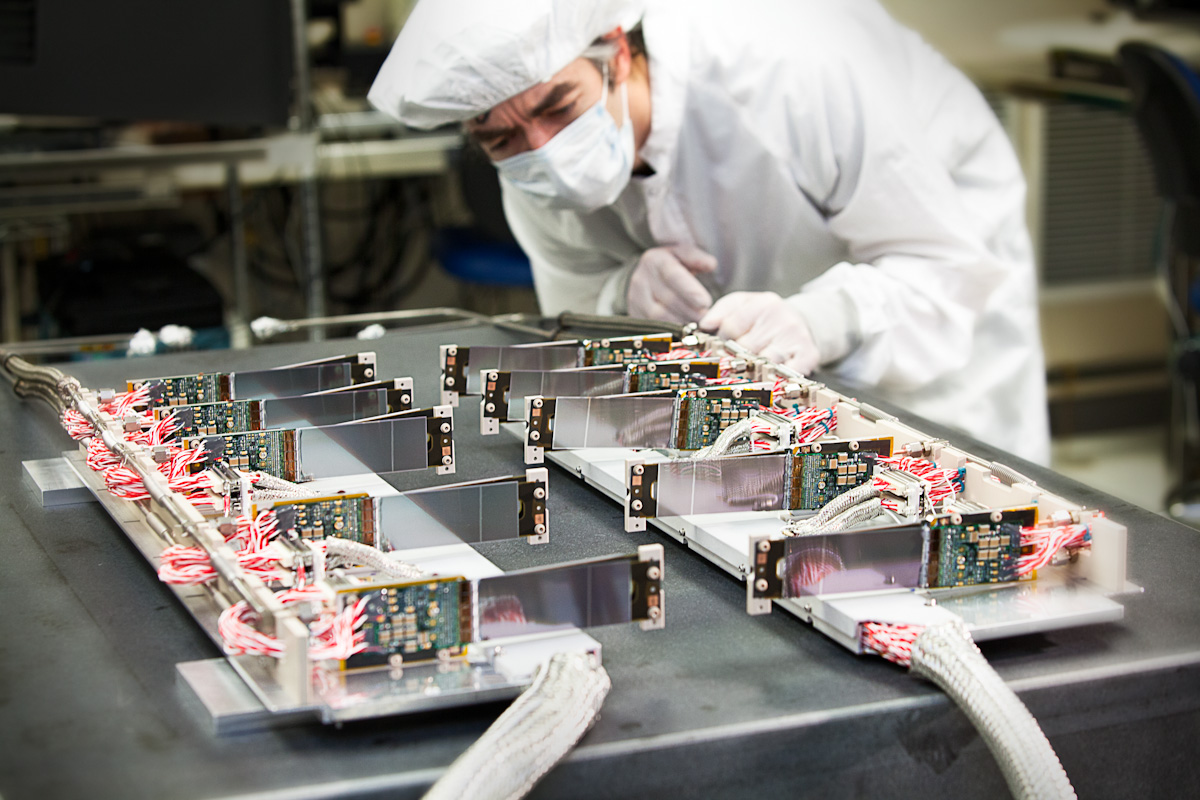
\includegraphics[width=7cm]{figures/2012-101-PHOTON-DETECTOR-001}
\caption{\small{Both halves of the HPS Test SVT after final assembly at SLAC.  The cooling manifolds and 
integrated cable runs are clearly seen.} }
\label{fig:tracker_halves}
\end{center}
%\vspace*{-5mm}
\end{figure}
%=======================

\subsection{Components}
The sensors for the SVT are $p+$-on-$n$, single sided, AC coupled, polysilicon-biased microstrip 
sensors fabricated on $<100>$ silicon and have 30 (60) micron sense (readout) pitch over their 
$4\times10$~cm$^2$ surface. This sensor technology was selected to match the requirement of 
a $<1$\% $X_0$ per layer, single-hit resolution better than 50~$\mu$m and tolerant of a radiation 
dose of approximately $1.5\times10^{14}$~\fluenceunit{} for a six month run. The sensors 
were purchased from the Hamamatsu Photonics Corporation for the cancelled 
Run 2b upgrade of the D\O~experiment~\cite{Denisov:2001aa} which satisfied the requirement that 
the technology must be mature and available within the time and budget constraints.

%\subsubsection{Front-end Electronics}
Despite having only small spots with very high occupancy (up to 4~MHz/mm$^2$) closest to the primary 
beam, the rates are still high and lowering the peak occupancy to 
approximately 1\% for tracking requires a trigger window and hit time tagging of roughly 8~ns. The 
ECal readout and trigger described in Sec.~\ref{sec:fadc} can achieve such resolution. To reach this 
performance the sensors for the SVT are readout by the APV25 ASIC developed for the CMS 
experiment at CERN~\cite{French:2001xb}. The APV25 can capture two successive samples of three 
of the output of the shaper at a sampling rate of approximately 40~MHz.  By fitting the known 
$CR$-$RC$ shaping curve to these samples, the initial time of the hit can be determined to a precision 
of 2~ns for S/N$\approx25$~\cite{Friedl:2009zz}.  For electron beam running, six-sample readout and 
the shortest possible shaping time (35~ns) is used to best distinguish hits that overlap in time.
The APV25 ASICs are hosted on simple FR4 hybrid readout boards, outside the tracking volume, with a 
short twisted-pair pigtail cable to provide power and configuration and signal readout. Along with a 
single sensor, these are glued to a polyamide-laminated carbon fiber composite backing making 
up a half-module. A window is machined in the carbon fiber leaving only a frame around the periphery 
of the silicon to minimize material. A 50~$\mu$m sheet of polyamide is laminated to the surface of the 
carbon fiber with 1~mm overhang at all openings to ensure good isolation between the backside of the 
sensor, carrying high-voltage bias, and the carbon fiber which is held near ground. 

The sensor modules for the SVT consist of a pair of identical half-modules, sandwiched back-to-back 
around an aluminum cooling block at one end and a similar PEEK spacer block at the other. 
Figure~\ref{fig:tracker_module} shows a single module after assembly.
%=======================
\begin{figure}[htp]
	\begin{center}
   	 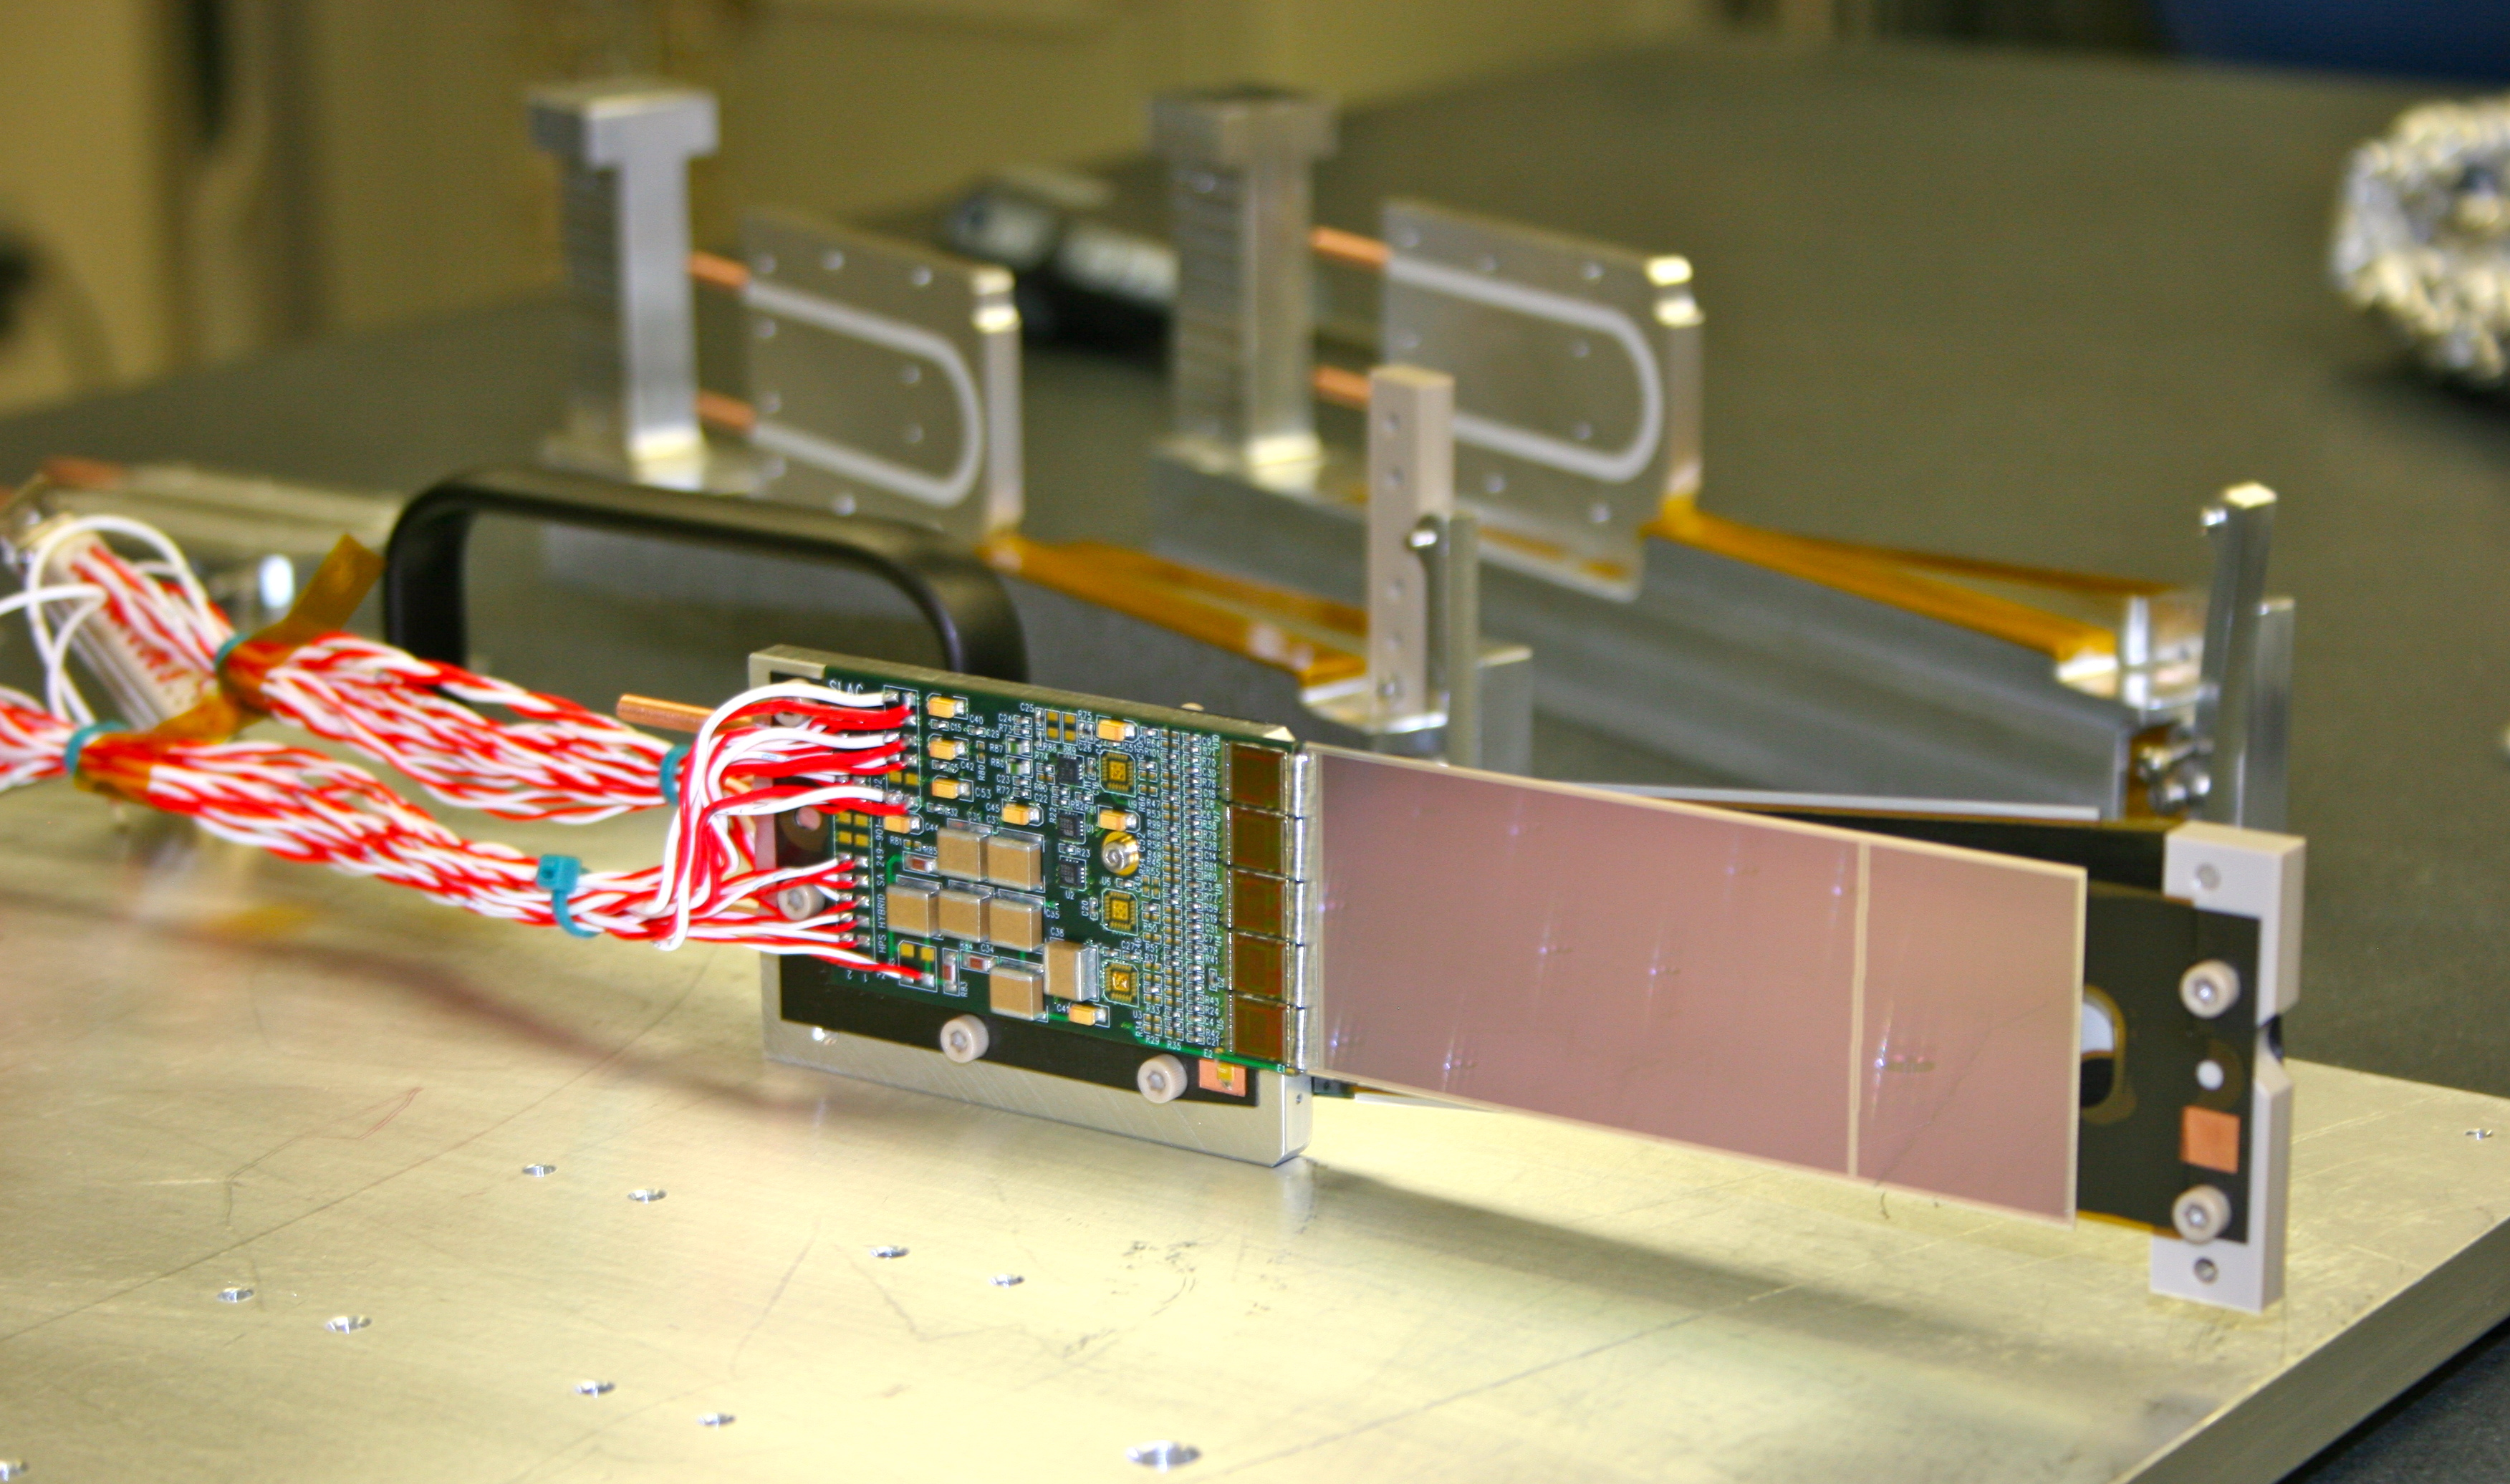
\includegraphics[width=7cm]{figures/IMG_5200}
	\caption{\small{A prototype module assembly (foreground) with the 50~mrad (left) and 100~mrad (right) module assembly fixtures in the background.  A pair of cooling blocks and a spacer block can be seen on the fixtures.} }
	\label{fig:tracker_module}
	\end{center}
\vspace*{-5mm}
\end{figure}
%=======================
The cooling block provides the primary mechanical support for the module as well as cooling via copper 
tubes pressed into grooves in the plates. The spacer block defines the spacing between the sensors at 
the far end of the module, stiffens the module structure, and improves the stability of the sensor 
alignment.  The average support material in the tracking volume is approximately 0.06\% $X_{0}$ per 
double-sided module for a total material budget of 0.7\% per layer.

The total SVT power consumption budget of about 50~W is removed by a water/glycol mixture 
circulated through a flexible manifold attached to the copper tubes in the cooling blocks. During the Test 
run the sensors where operated at around $23^{\circ}$C. The power consumption is dominated by five 
APV25 ASICs on each hybrid board consuming approximately 2~W, radiant heat load is less than 
0.5~W per sensor and leakage current is only significant in a small spot after irradiation.  







\subsection{Production, Assembly and Shipping}

%Of the sensors tested during production, 90\% were capable of 1000~V bias voltage without breakdown. 
Hybrids with APV25 ASICs underwent quick qualification testing and each half-module was run at low 
temperature ($\approx5^{\circ}$ C) and fully characterized for pedestals, gains, noise and time response 
after assembly.  Of 29 half-modules built, 28 passed qualification testing, leaving 8 spare modules after 
completion of the SVT, all capable of 1000~V bias voltage without breakdown.  Full-module assembly 
and mechanical surveys were performed at SLAC before final assembly, testing and shipping of the 
SVT to JLab. A custom shipping container with nested crates and redundant isolation for shock and 
vibration was built in order to safely send the partly assembled SVT to JLab. At JLab, the entire SVT was 
integrated with the full DAQ and the power supplies before moving the module-loaded support plates to 
Hall B for final mechanical assembly and installation inside of the vacuum chamber.

\subsection{Alignment}
The SVT was aligned using a combination of optical, laser and touch probe surveys at SLAC and JLab. 
The optical survey of individual modules with precision of a few $\mu$m are combined with a 
touch-probe survey of the overall SVT support structure, with 25-100~$\mu$m precision, to locate the 
silicon sensor layers with respect to the support plates and the mechanical survey balls on the base 
plate. After full assembly and installation of the SVT at JLab, a mechanical survey of the SVT base plate 
position inside the pair spectrometer vacuum chamber is used to determine the global position of the 
SVT with respect to CEBAF beam line. The resulting survey-based alignment has the position of the 
silicon sensors correct to within a few hundred microns measured from tracks in the Test run data. 
A more sophisticated global track-based alignment technique to reach final alignment precision 
well below 50~$\mu$m is being developed.


%%%%%%%%%%%%%%%%%%%%%%%%%%%%%%%%%%%%%%%%%%%%%%%%%%


\section{Electromagnetic Calorimeter}
\label{sec:ecal}

The electromagnetic calorimeter (ECal), installed downstream of the PS dipole magnet, performs two 
essential 
functions for the experiment: it provides a trigger signal to select what events to read out from the 
detector sub-systems and is used in the analysis to identify electrons and positrons. 
The technology and design choices are largely driven by the need for a compact forward design 
covering the SVT \Aprime acceptance and able to fully absorb 
electrons and positrons with energy between $0.5$-$6.5$~GeV, fine granularity and signal 
readout speed to handle 1~MHz/cm$^{2}$ of electromagnetic background and remain operable 
after a radiation dose larger than $X$~MRad. The lead-tungstate (PbOW$_{4}$) crystal inner 
calorimeter of the CLAS detector~\cite{2008erhm.conf..421N} in operation since 2005 in Hall B meets 
all the requirements set by HPS. The modules from this calorimeter have been subsequently 
repurposed for HPS. 


\subsection{Components}

The ECal module shown in Fig.~\ref{fig:ecal-module} is based on a tapered 160~mm long 
lead-tungstate (PbWO$_{4}$) crystal with a $13.3\times13.3$~mm$^2$ ($16\times16$~mm$^2$) front 
(rear) face wrapped in VM2000 multilayer polymer mirror film. 
\begin{figure}[]
\begin{center}
{\small
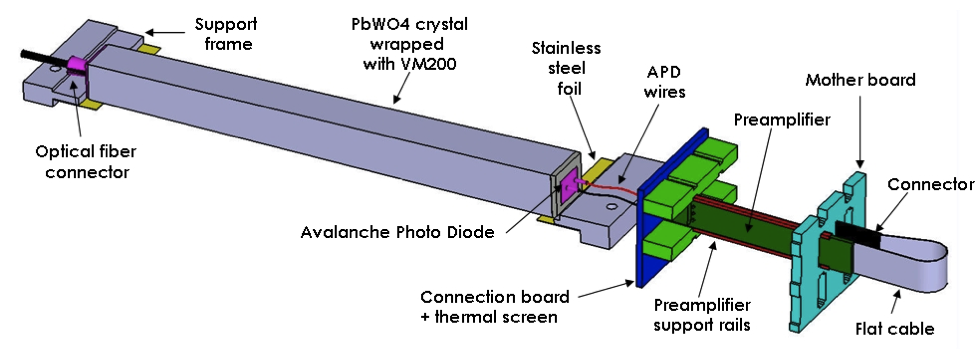
\includegraphics[width=7cm]{figures/ecal-module-schematic.png}
\caption{Schematic vied of an ECal module.}
\label{fig:ecal-module}
}
\end{center}
\end{figure}
The scintillation light, approximately $X$ photoelectrons/MeV, is readout by a 
5$\times$5~mm$^2$ Hamamatsu S8664-55 Avalanche Photodiode (APD) with 75\% quantum 
efficiency glued to the rear face surface using MeltMount 1.7 thermal plastic adhesive. 
The low gain of APDs ($\sim 200$) was compensated with custom made preamplifier boards, which 
provide factor of 2000 amplification of the APD signal.

\subsection{Layout}
Similar to the SVT, the ECal is built in two separate halves that are mirror reflections of one another 
about the plane of the nominal electron beam to avoid interfering with the 15~mrad "dead zone". 
As shown in Fig.~\ref{fig:ecal}, the 221 modules, supported by aluminum support frames, in each half 
are arranged in rectangular formation with 5 layers and 46 crystals/layer except for the layer closest to 
the beam where 9 modules were removed to allow a larger opening for the outgoing electron and 
photon beams. Each half was enclosed in a temperature controlled box ($<1^{\circ}$~F stability and 
$<4^{\circ}$~F uniformity) to stabilize the crystal light yield and the operation of the APDs and its 
preamplifiers. 
Four printed circuit boards mounted on the backplane penetrated the enclosure and was used to 
supply the $\pm 5$~V operating voltage for the preamplifiers, 400~V bias voltage to the APDs, and to 
read out signals from the APDs. Each half of the ECal was divided into 12 bias voltage groups with a 
gain uniformity of about 20\%. 

During the Test run, both halves were held in place by four vertical bars attached to an above rail, 
placing the front face of the crystals 147~cm from the upstream edge of the magnet and with a 
8.7~cm gap between the innermost edge of the crystals in the two halves.
{\small
\begin{figure}[]
\begin{center}
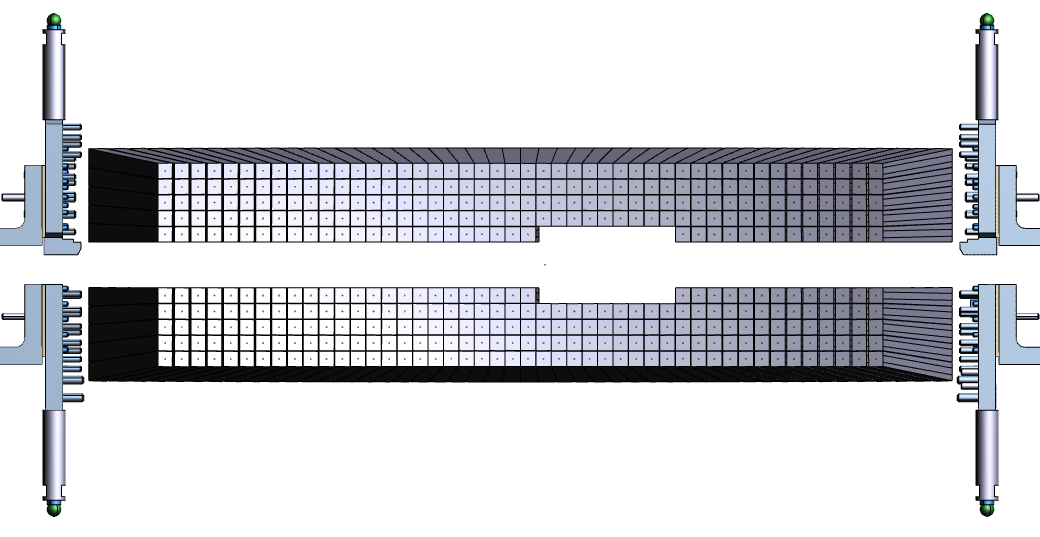
\includegraphics[width=0.45\textwidth]{figures/ECal}
%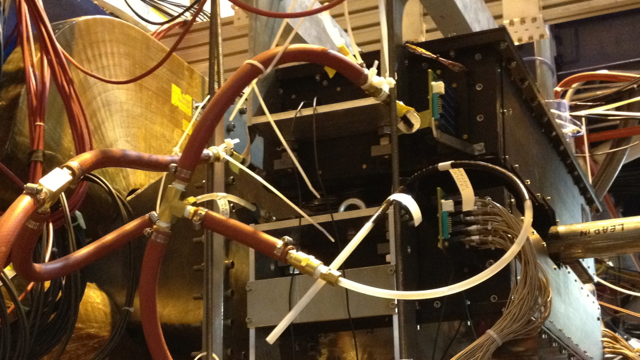
\includegraphics[width=0.45\textwidth]{figures/ecal_picture_beamline}
\caption{Rendered layout view of the ECal looking downstream.}
\label{fig:ecal}
\end{center}
\end{figure}
}


\subsection{Signal readout}
\label{sec:fadc}
After a 2:1 signal splitter, $1/3$ of an amplified APD signal ($2/3$ is sent to a timing module) is fed to a 
single channel of a JLab flash ADC (FADC) board~\cite{fadc}.
%\begin{figure}[]
%\begin{center}
%{\small
%\includegraphics[width=4cm]{figures/FADC250_Photo_001.jpg}
%\caption{The JLab FADC250 VXS module.}
%\label{fig:fadc}
%}
%\end{center}
%\end{figure}
The FADC boards are high speed VXS modules digitizing up to 16 APD signals 
at 250~MHz and storing samples in 8~$\mu$s deep pipelines with 12-bit resolution. 
When a trigger is received, the part 
of the pipeline from 5 samples before and 30 after the signal crossed a programmable 
threshold (for the Test run this was set to $\approx70$~MeV) are 
summed and stored in a 17-bit register for readout. In addition a 4~ns resolution timestamp of the 
threshold crossing is reported in the readout for each pulse.
This scheme significantly compresses the data output of the FADC. During offline data analysis, a 
calibrated pedestal value is subtracted to obtain the actual summed energy.
Two 20-slot VXS crates with 14 (13) FADC boards were employed in the Test run to read out the top 
(bottom) half of the ECal.
In the Test run 385 out of 442 modules (87\%) were used in offline reconstruction, 39 modules were 
disabled or not read out (no FADC channel available, no APD bias voltage or masked out due to 
excessive noise) and 18 were masked offline due to noise. 
%\begin{figure}[]
%\begin{center}
%{\small
%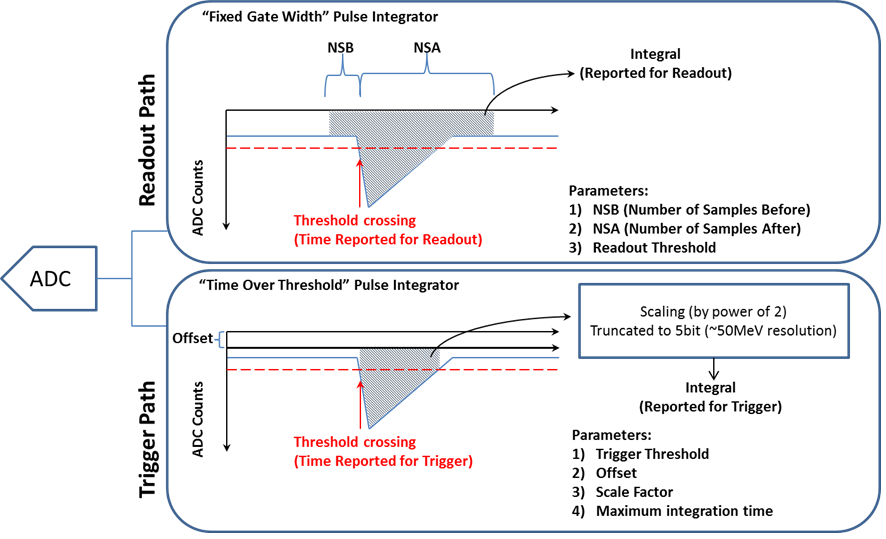
\includegraphics[width=8cm]{figures/fadc_datapath_diagram.png}
%\caption{The two different readout modes of the FADC used in the Test run.}
%\label{fig:hps_trigger_data}
%}
%\end{center}
%\end{figure}


%%%%%%%%%%%%%%%%%%%%%%%%%%%%%%%%%%%%%%%%%%%%%%%%%%


\section{Trigger and Data Acquisition}
\label{sec:triggerdaq}

The DAQ system handles acquisition of data from the ECal and SVT sub-detectors  with 
two DAQ architectures. The SVT DAQ is based on Advanced Telecom Communications Architecture 
(ATCA) hardware while the ECal uses VMEbus Switched Serial (VXS) based hardware. Data from the 
sub-detectors are only 
readout when a trigger signal from the trigger system is received formed on input from the ECal. 
\subsection{Trigger system}
\label{sec:trigger}

The trigger system is designed to select time coincidences of electromagnetic clusters in the 
top and bottom halves of the ECal. Figure~\ref{fig:hps_trigger_cal} shows a schematic overview 
of each stage of the system. 
 \begin{figure}[b]
\begin{center}
{\small
 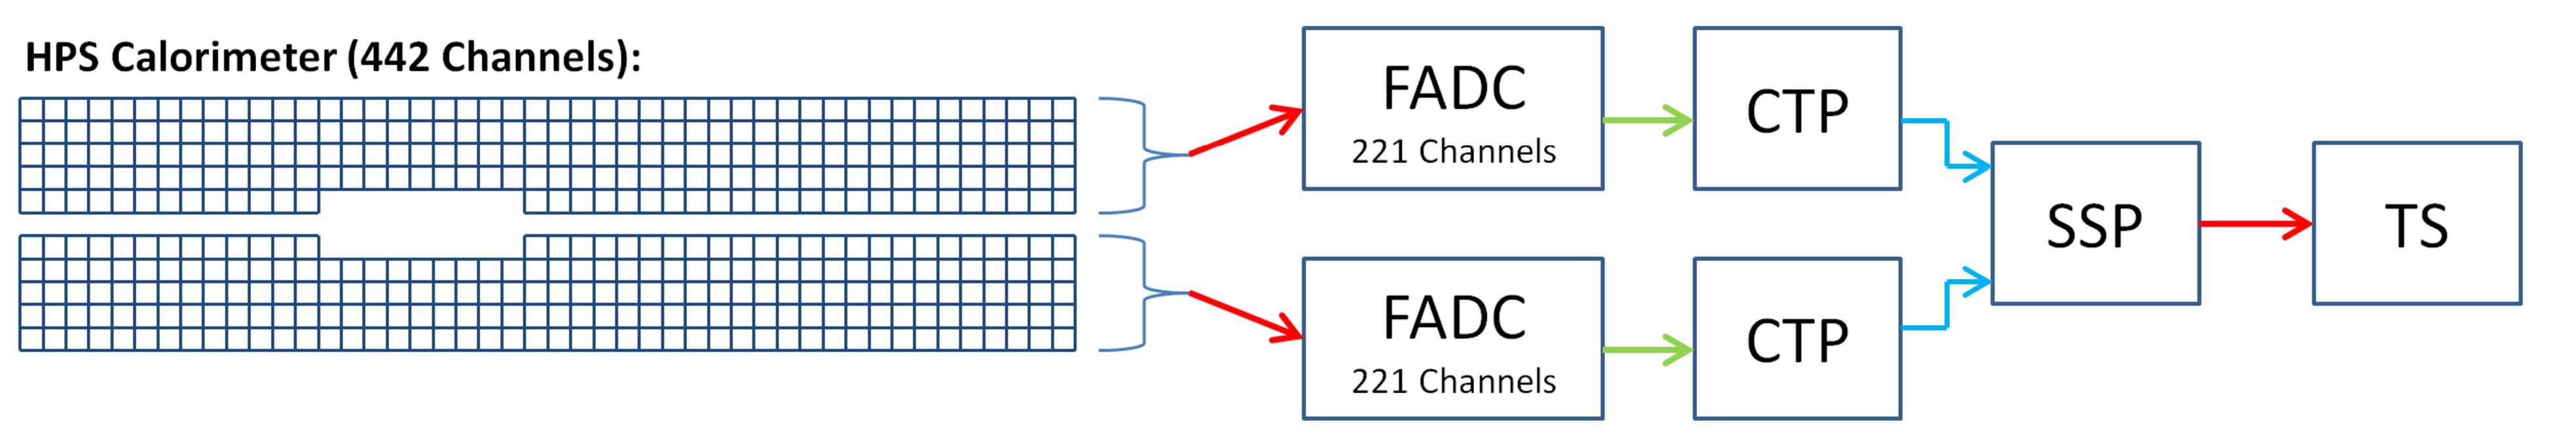
\includegraphics[width=8cm]{figures/hps_trigger_cal}
\caption{Block diagram of the ECAL trigger system consisting of the FADC that samples and digitizes 
signals for each detector channel and sends them for cluster finding in the CTP. The CTP clusters are 
sent to the SSP where the final trigger decision is taken based on pairs of clusters in both halves of the 
ECal. The decision is sent to the Trigger Supervisor (TS) that generates the necessary signals to readout 
the sub-detectors.}
 \label{fig:hps_trigger_cal}
}
\end{center}
 \end{figure}
Each channel on the FADC board has an independent data path to send 5-bit pulse energy and 3-bit 
pulse arrival time information every 32~ns to a trigger processing board (CTP), which is in the same 
crate. The 3-bit pulse arrival time allows the trigger to know the pulse timing at 4~ns resolution. 
Contrary to the readout path 
described in Sec.~\ref{sec:fadc}, this energy is a pedestal subtracted time-over-threshold sum with 
programmable offsets and minimum threshold discriminator for each channel. With input from all 
FADC channels, i.e. one half of the ECal, the CTP performs cluster finding and calculates cluster 
energy, shape and timing information. The 3x3 fixed-window, highly parallel, FPGA-based cluster 
algorithm simultaneously searches for up to 125 clusters with energy sum larger than 
the programmable energy threshold ($\approx270$~MeV). Crystals in the 
fixed-window are included in the sum if the leading edge of the pulse occurred within a 32~ns time 
window to take into account clock skew and jitter throughout the system.
The CTP only accepts clusters with the highest energy 3x3 window locally to deal with overlapping and 
very large clusters. The sub-system board (SSP) receives the clusters from the top and bottom half CTP 
at a maximum of 250MHz and searches for pairs of clusters in a 8 ns wide coincidence window. The 
SSP sends triggers to the trigger supervisor (TS), which generates all the necessary signals and 
controls the entire DAQ system readout through the trigger interface units installed in every crate that 
participate in the readout process.

The trigger system is free-running and driven by the 250~MHz global clock and has essentially zero 
dead time at the occupancies expected for HPS. The trigger supervisor can apply dead time if 
necessary, for example on a `busy' or `full' condition from the front-end electronics. The system is 
designed to handle trigger rates above 50~kHz and has a latency set to $\approx 3~\mu$s to match 
that required by the SVT APV25 ASIC. During the Test run, for the most part the trigger system 
required only a single cluster in either the top or bottom Ecal halves and was tested to trigger rates 
above 100~kHz by lowering thresholds. 



\subsection{SVT Data Acquisition}
%igitization, Event Building and Data Transmission}
\label{sec:svt_daq}
The SVT DAQ is based on the Reconfigurable Cluster Element (RCE) and cluster 
interconnect concept developed at SLAC as generic building blocks for DAQ systems. 
The RCE is a generic computational building block, housed on a separate daughter card called 
Data Processing Module (DPM), that are realized on an ATCA front board called the Cluster On Board 
(COB), see Fig.~\ref{fig:cob}.
 \begin{figure}[]
\begin{center}
{\small
	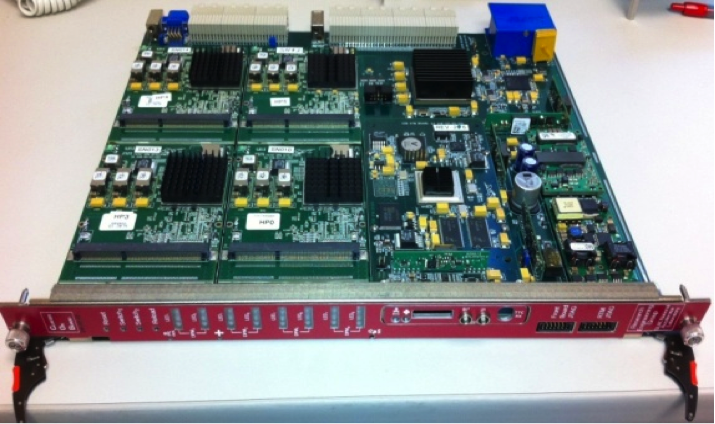
\includegraphics[width=6cm]{figures/svt_daq_module}
	\caption{The SVT DAQ COB board with four data processing daughter cards (DPMs) visible on the left side.}
	\label{fig:cob}
}
\end{center}
\end{figure}
The first generation RCE used in the Test run consisted of a Virtex~5 FPGA with 1~GB of DDR3 RAM. 
A schematic overview of the system is shown in Fig.~\ref{fig:svtdaq}. 
 \begin{figure}[]
\begin{center}
{\small
	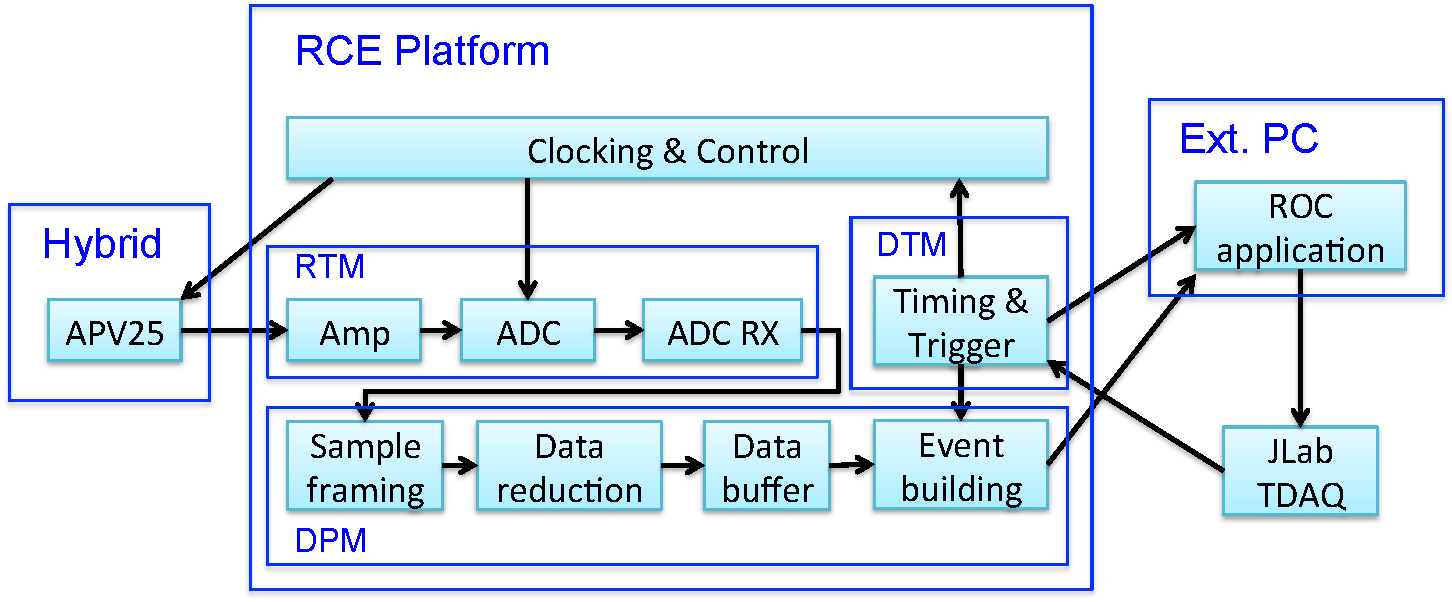
\includegraphics[width=8cm]{figures/svt-daq-sketch}
	\caption{Block diagram overview of the SVT DAQ.}
	\label{fig:svtdaq}
}
\end{center}
\end{figure}
The analog outputs of up to 12 SVT half-modules (60 APV25 ASICs) are digitized on the Rear-Transition-
Module (RTM), a custom board 
on the back side of the ATCA crate, interfacing the HPS-specific readout to the generic DAQ components 
on the 
COB. A pre-amplifier converts the APV25 differential current output to a different voltage output scaled to 
the sensitive range of a 14-bit ADC operating at the system clock of 41.667~MHz. The RTM is organized 
into four sections with each section supporting three SVT half-module hybrids (15 APV25 ASICs). The 
RTM also includes a 4-channel fiber optic module and supporting logic which is used to interface 
to the JLab trigger system supervisor. Each section of the RTM is input to a DPM which apply thresholds 
for data reduction and organizes the sample data into UDP datagrams. The DPM also hosts an I$^{2}$C 
controller used to configure and monitor the APV25 ASICs. A single ATCA crate with two COB cards 
was used, one supporting four DPMs and one supporting 3 DPMs and one DPM that is configured as 
the trigger and data transmission module. The two COB cards and their DPMs are interconnected with a 
10Gb/s switch card~\cite{Larsen:2011zb} which also hosts two 1Gb/s Ethernet interfaces to the external 
SVT DAQ PC.  

The external PC supports three network interfaces; two standard 1Gb/s Ethernet and one custom low 
latency data reception card. The first is used for slow control and monitoring of the 8 
DPM modules and the second serves as the interface to the JLAB data acquisition system. The third 
custom low latency network interface is used to receive data from the ATCA crate and supports a low 
latency, reliable TTL trigger acknowledge interface to the trigger DPM. This PC hosts the SVT control 
and monitoring software as well as the Read Out Controller application used to interface with the 
JLab DAQ.

In order to minimize cable length for the analog APV25 output signal the ATCA crate was located 
approximately 1~m from the beam line, next to our cable vacuum feed-troughs.   
Before shielding with lead-blankets was arranged, we observed two failures of normally reliable ATCA 
crate power supplies, time-correlated to beam instabilities. 

While trigger rates during the Test run was significantly lower this system was tested at trigger rates up 
to 20~kHz and 50~MB/s. 



\subsection{General Data Acquisition and Online Computing}
\label{sec:daq}
Every crate participating in the readout process contains a Readout Controller (ROC) that 
collects digitized information, processes it, and sends it on to the event builder. For the ECal, both 
VXS crates run ROC applications in a single blade Intel-based CPU module running CentOS 
Linux OS. For the SVT DAQ, the ROC application runs on the external PC under RHEL. 
The event builder assembles information from the ROCs into a single event which is passed to the 
event recorder that writes it to a RAID5-based data storage system capable of handling up to 
100~MB/s. The event builder and other critical components run on multicore Intel-based multi-CPU 
servers. The DAQ network system is a network router providing 10Gbit/s high-speed connection 
to the JLab computing facility for long-term storage. For the Test run, both the SVT and ECal ROC had a 
1Gbit/s link to the network router.




%%%%%%%%%%%%%%%%%%%%%%%%%%%%%%%%%%%%%%%%%%%%%%%%%%


\section{Performance}

\subsection{SVT Performance}

For the duration of the Test run all SVT modules and APV25 chips were configured to their 
nominal operating points~\cite{Jones:1069892} with all sensors reverse-biased at 180~V.  The 
sensors were operated within a temperature range of  $20-24^\circ$C.
Approximately 97\% of the 12,780 SVT channels were found to
be operating normally;  the fraction of dead or noisy channels varied from 2.4\% to 4.7\% throughout 
the Test run. Most of these losses were due to 2-4 misconfigured APV25 ASICs, a known noisy 
half-module and problems in two particular APV25 ASICs. 


\subsubsection{Cluster and Hit Reconstruction}

After a trigger is received, the amplitude  of every  APV25 analoge output  is sampled and digitized in 
six consecutive time bins, separated by roughly 25~ns.  
The typical pulse shape obtained is shown in Fig.~\ref{fig:pulse_shape}. As the figure demonstrates,  
the SVT was well timed-in to the trigger with the rise of the pulse at the 3rd sampling 
point. Note that in the Test run the APV25 ASICs were operating with a 50~ns shaping time.  
\begin{figure}[]
\begin{center}
{\small
	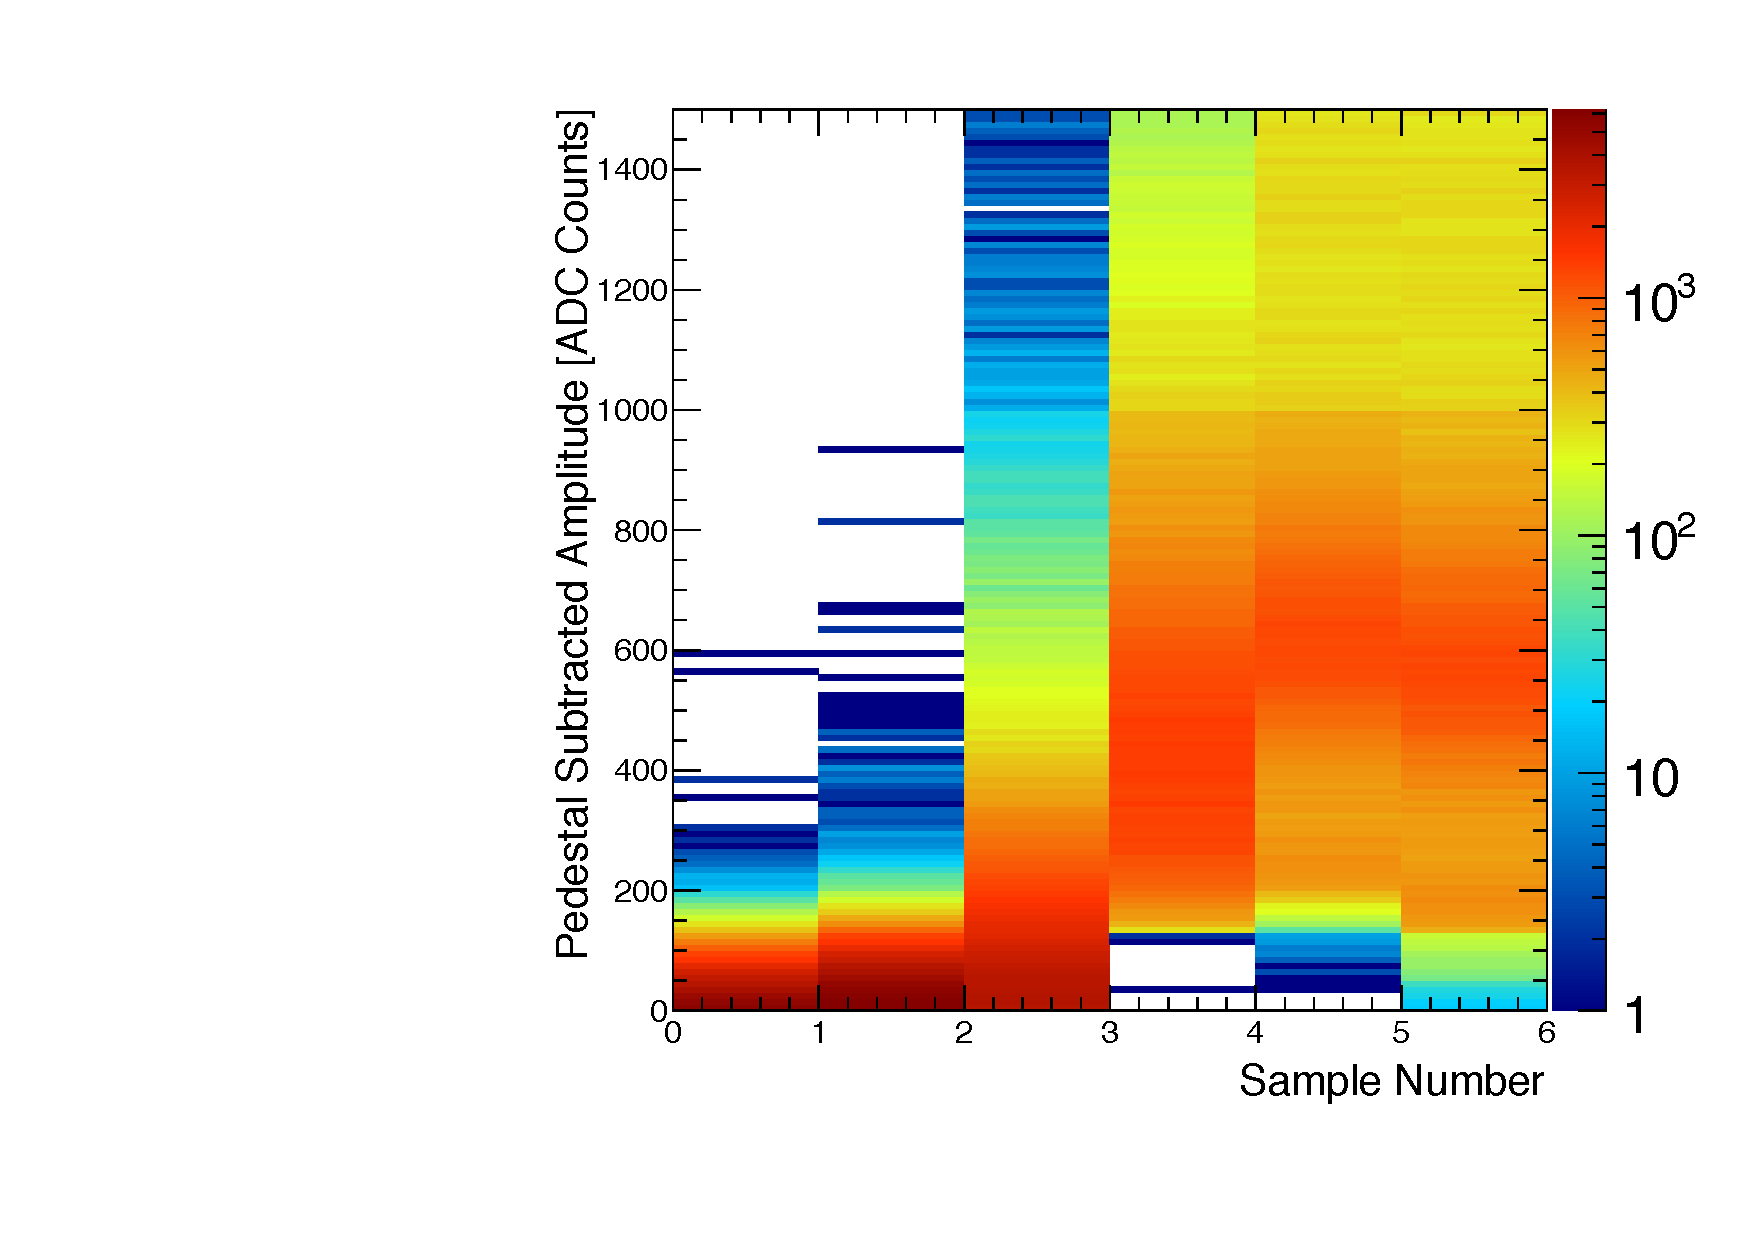
\includegraphics[width=6cm]{figures/run1351_110513_samples_L1_top.pdf}
	\caption{Accumulation of six pedestal-subtracted samples from individual SVT channels associated 
	with hits on tracks.}
	\label{fig:pulse_shape}
}
\end{center}
\end{figure}
These hits are passed through a simple clustering algorithm which forms clusters by grouping adjacent 
strips with the position of a cluster on the sensor determined by the amplitude-weighted mean.
With a linear gain up to $\approx 3$~MIPs, the cluster charge for hits associated with a track follow 
the characteristic Landau shape. 
%, see Fig.~\ref{fig:cluster_pulse}.  
A noise level between $1.1-1.5\times 10^{3}$ electrons was established through multiple calibration 
runs giving a signal to noise ratio of $21-25$. Lab-based radioactive source tests was used to 
provide the absolute charge normalization.
%\begin{figure}[]
%\begin{center}
%{\small
%	%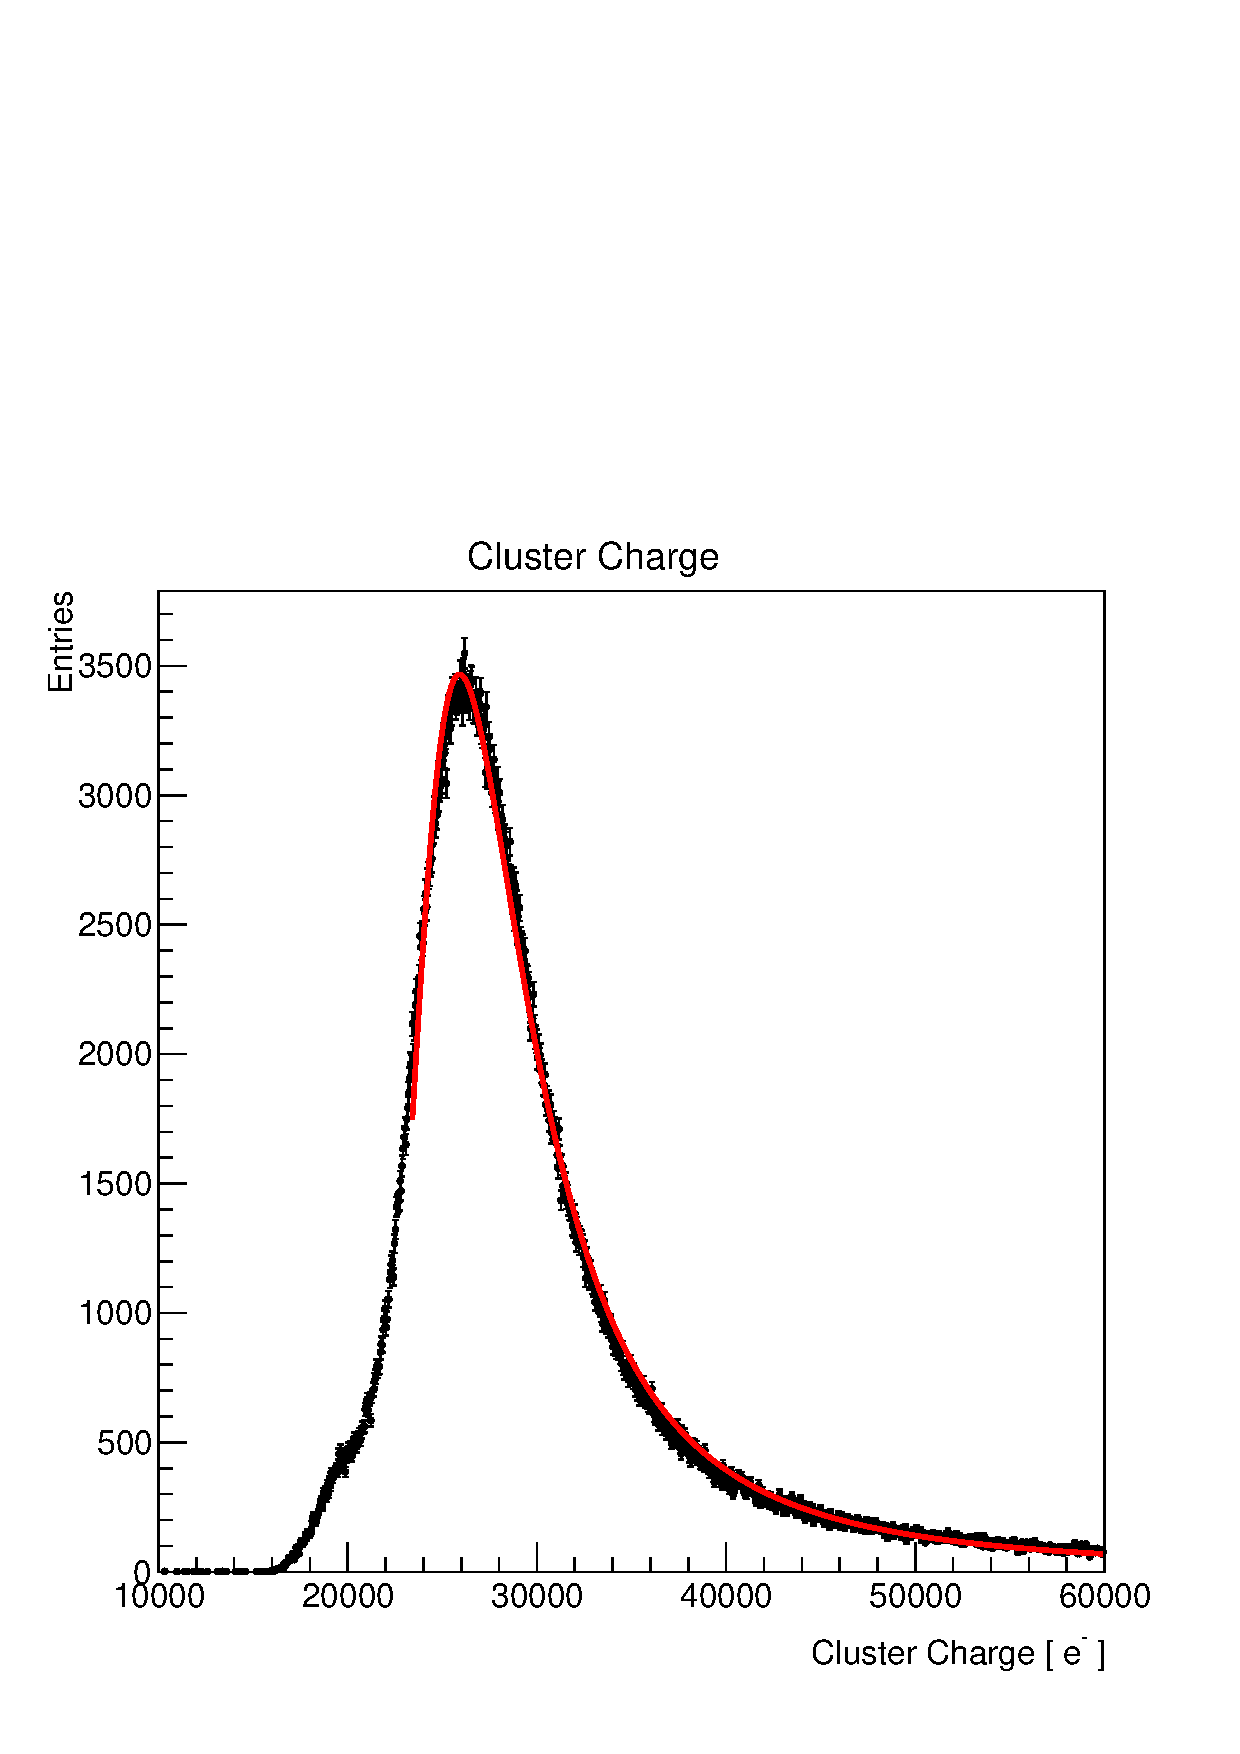
\includegraphics[width=7cm]{figures/run1351_mip_small.pdf}
%	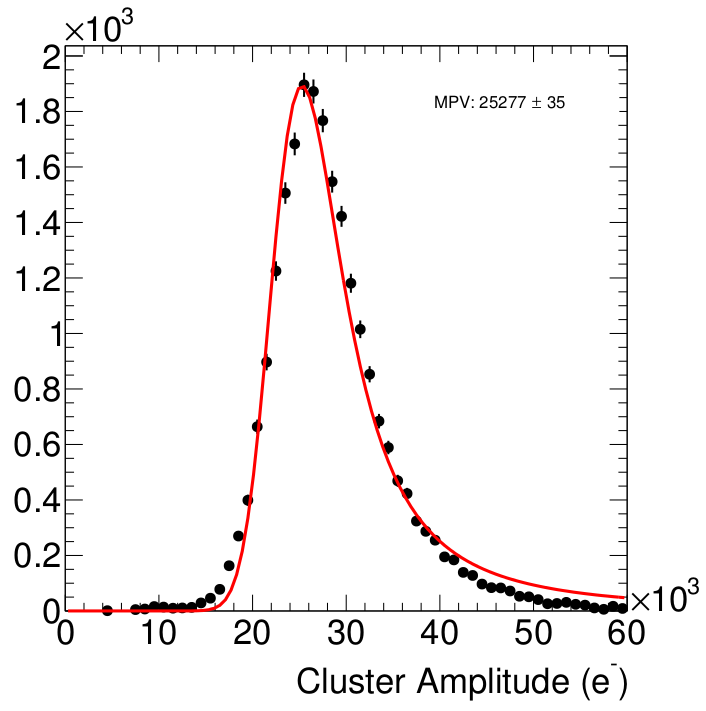
\includegraphics[width=7cm]{figures/mip_top_layer_2.png}
%    	\caption{ The cluster charge distribution for hits associated with a track. }
%	\label{fig:cluster_pulse}
%}
%\end{center}
%\end{figure}


In order to find the time, $t_0$, and amplitude of each hit, the six samples from each channel are fitted 
to an ideal $CR-RC$ function. After clustering hits on a sensor, the hit time for each cluster is computed 
as the amplitude-weighted average of the individually fitted $t_0$ on each channel. The 
$t_0$-resolution is studied by comparing the cluster hit time with the average of all cluster hit times on 
the track, see Fig.~\ref{fig:tracktime}. 
\begin{figure}[]
\begin{center}
{\small
	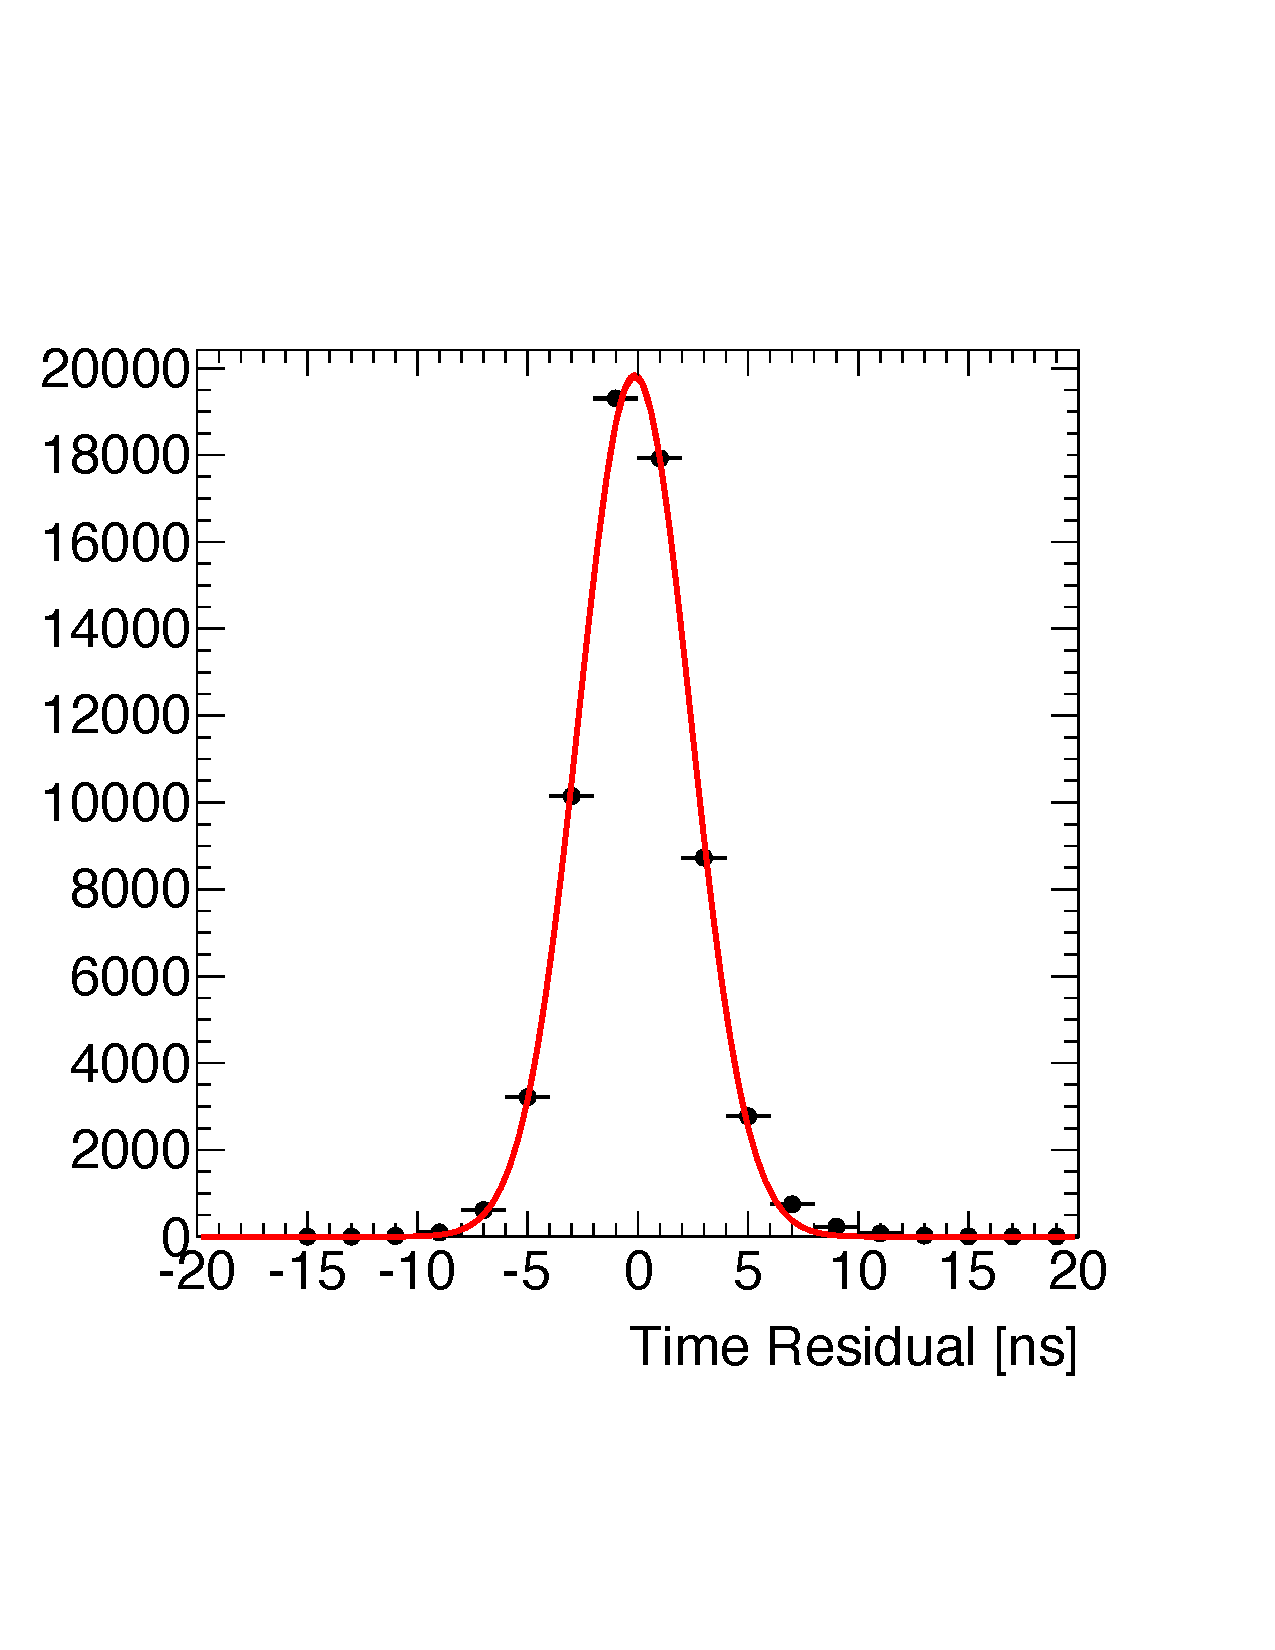
\includegraphics[width=7cm]{figures/test_run_1351_hit_time_corrected_top_layer2_mod.pdf}
	\caption{
	The residual of individual cluster times with the average of all clusters on the track. }
	\label{fig:tracktime}
}
\end{center}
\end{figure}
After correcting for offsets from each sensor (time-of-flight, clock phase) and accounting for the 
correlation between the $t_0$ and track time,  the extracted $t_0$ resolution is 2.6~ns. This is somewhat 
worse than the approximately 2~ns resolution expected for S/N~25 which we attribute to the true 
pulse shape differing from our idealized fit function which will be improved in the future. Reducing the 
APV25 ASIC pulse shaping time will also improve time resolution. 
These results show that we can operate with the six sample readout mode of the APV25 chip and 
achieve time resolution adequate for pileup rejection during electron running in HPS. 

While occupancy was slightly larger than expected, good agreement between data and simulation was 
found after taking into account dead or noisy channels. The hit efficiency was estimated by measuring 
the number of good tracks with a hit close to the extrapolated intersection of a given sensor that was 
excluded from the track fit itself. Tracks which intersect regions with known bad channels or very close to 
in the edge region are excluded. The hit efficiency, see Fig.~\ref{fig:hit_efficiency}, was measured to be 
above 98\% and fairly uniform across the SVT.
\begin{figure}[]
\begin{center}
{\small
    	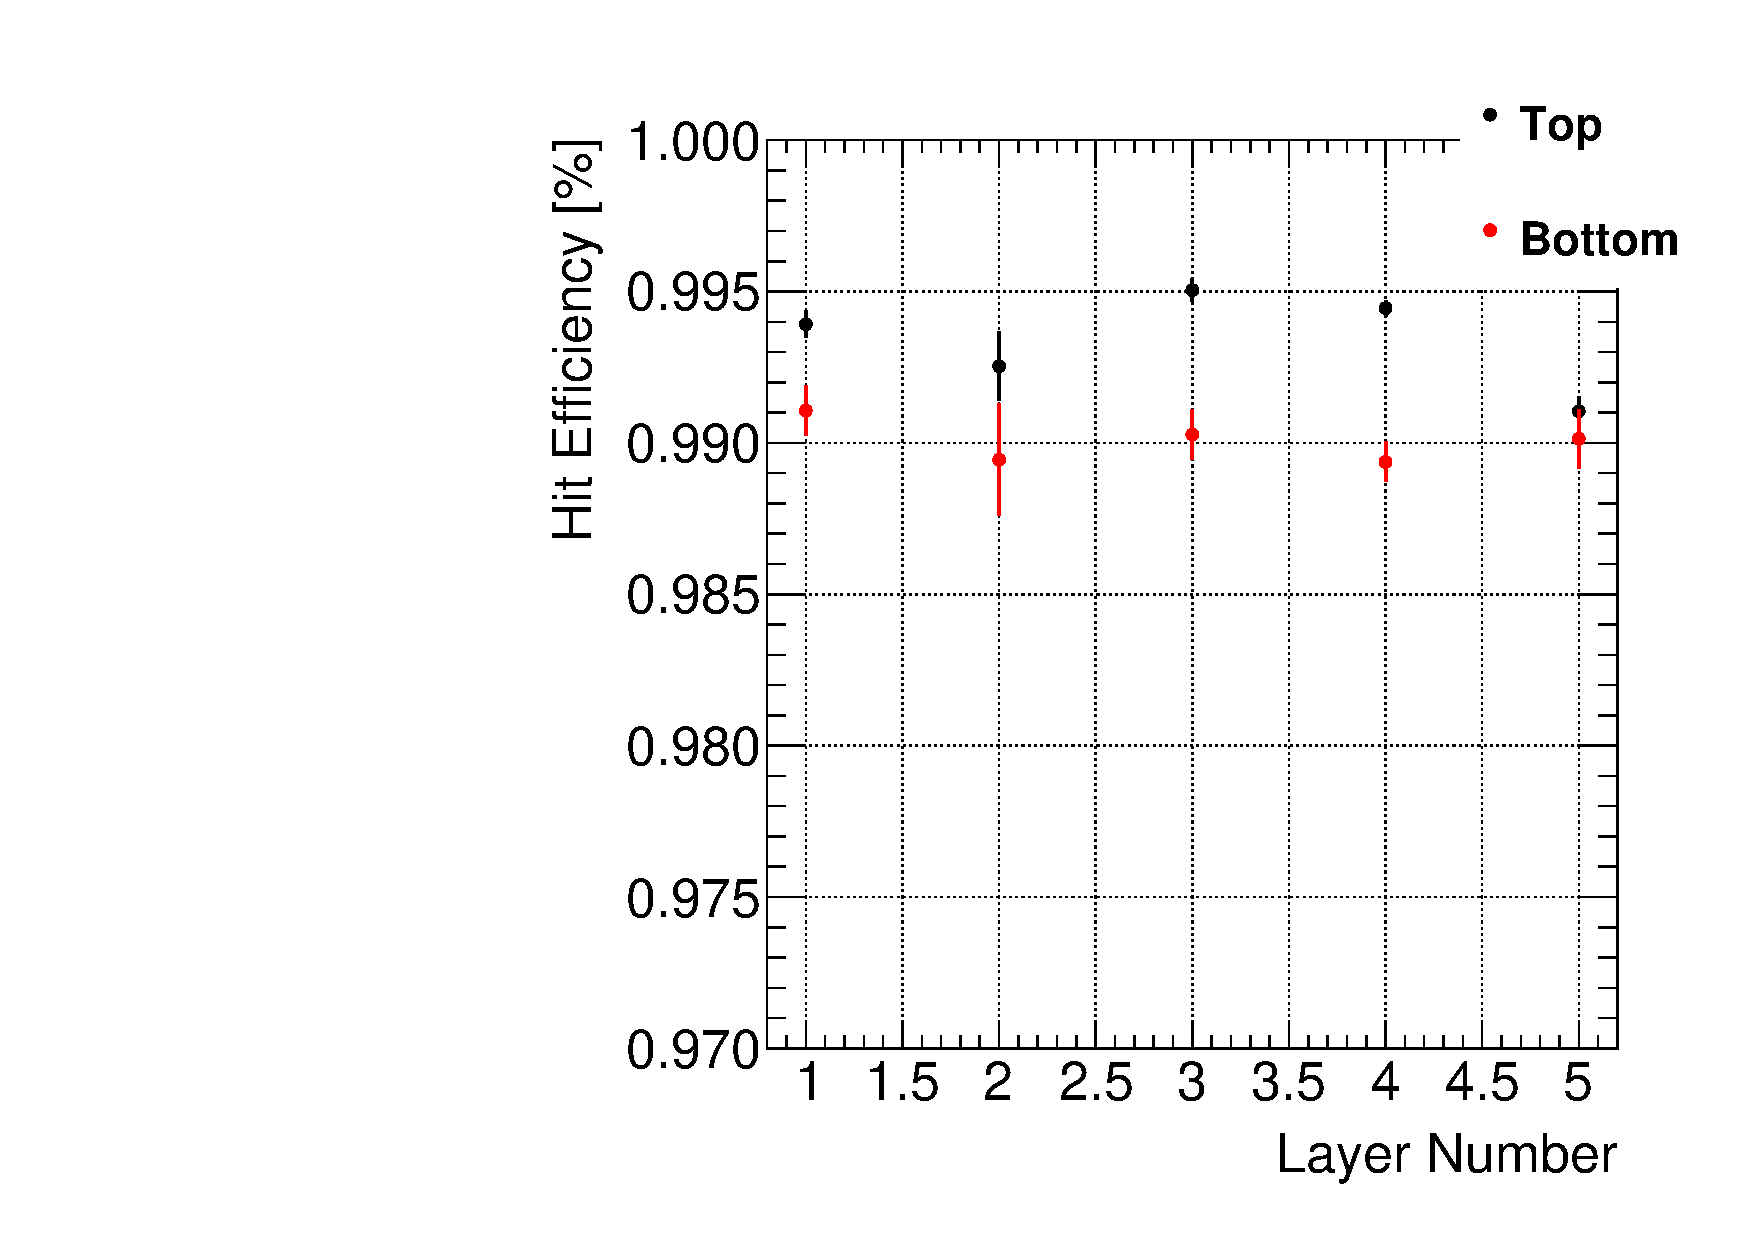
\includegraphics[width=7cm]{figures/single_hit_efficiency_Omar_11192013.pdf}
        \caption{ The hit reconstruction efficiency as a function of detector layer.}
	\label{fig:hit_efficiency}
}
\end{center}
\end{figure}
The spatial resolution of similar microstrip sensors is well established by test beam data, against which 
the charge deposition model in the simulation is validated.  This resolution can be parameterized as a 
function of the total signal to single-strip noise and the crossing angle of tracks through the sensor.  
The single-hit resolution for charged particles with signal to noise ratio above 20, as demonstrated 
here, is relatively constant at approximately 6~$\mu$m for tracks that enters approximately normal to the 
sensors as in HPS.



\subsubsection{Momentum and Vertexing Resolution}

By selecting \ee{} pairs from the triggered events we are able to study basic distributions of pair 
production kinematics. Pairs of oppositely charged tracks, one in the top and one in the bottom half of 
the SVT, with momentum larger than 400~MeV were selected. The pair production kinematics are 
relatively well reproduced as shown in Fig.~\ref{fig:pair_kin}. 

The expected momentum resolution from simulation is between 4-5\% for tracks in the momentum 
range of the Test run. By looking at the agreement 
between data and simulation in the shape of the kinematic distributions for single- and two track 
events and adjusting the overall momentum scale and smearing simulated events with a 
Gaussian resolution we estimate an agreement with the nominal scale and resolution to within 10\%.
 \begin{center}
{\small
\begin{figure*}[t]
   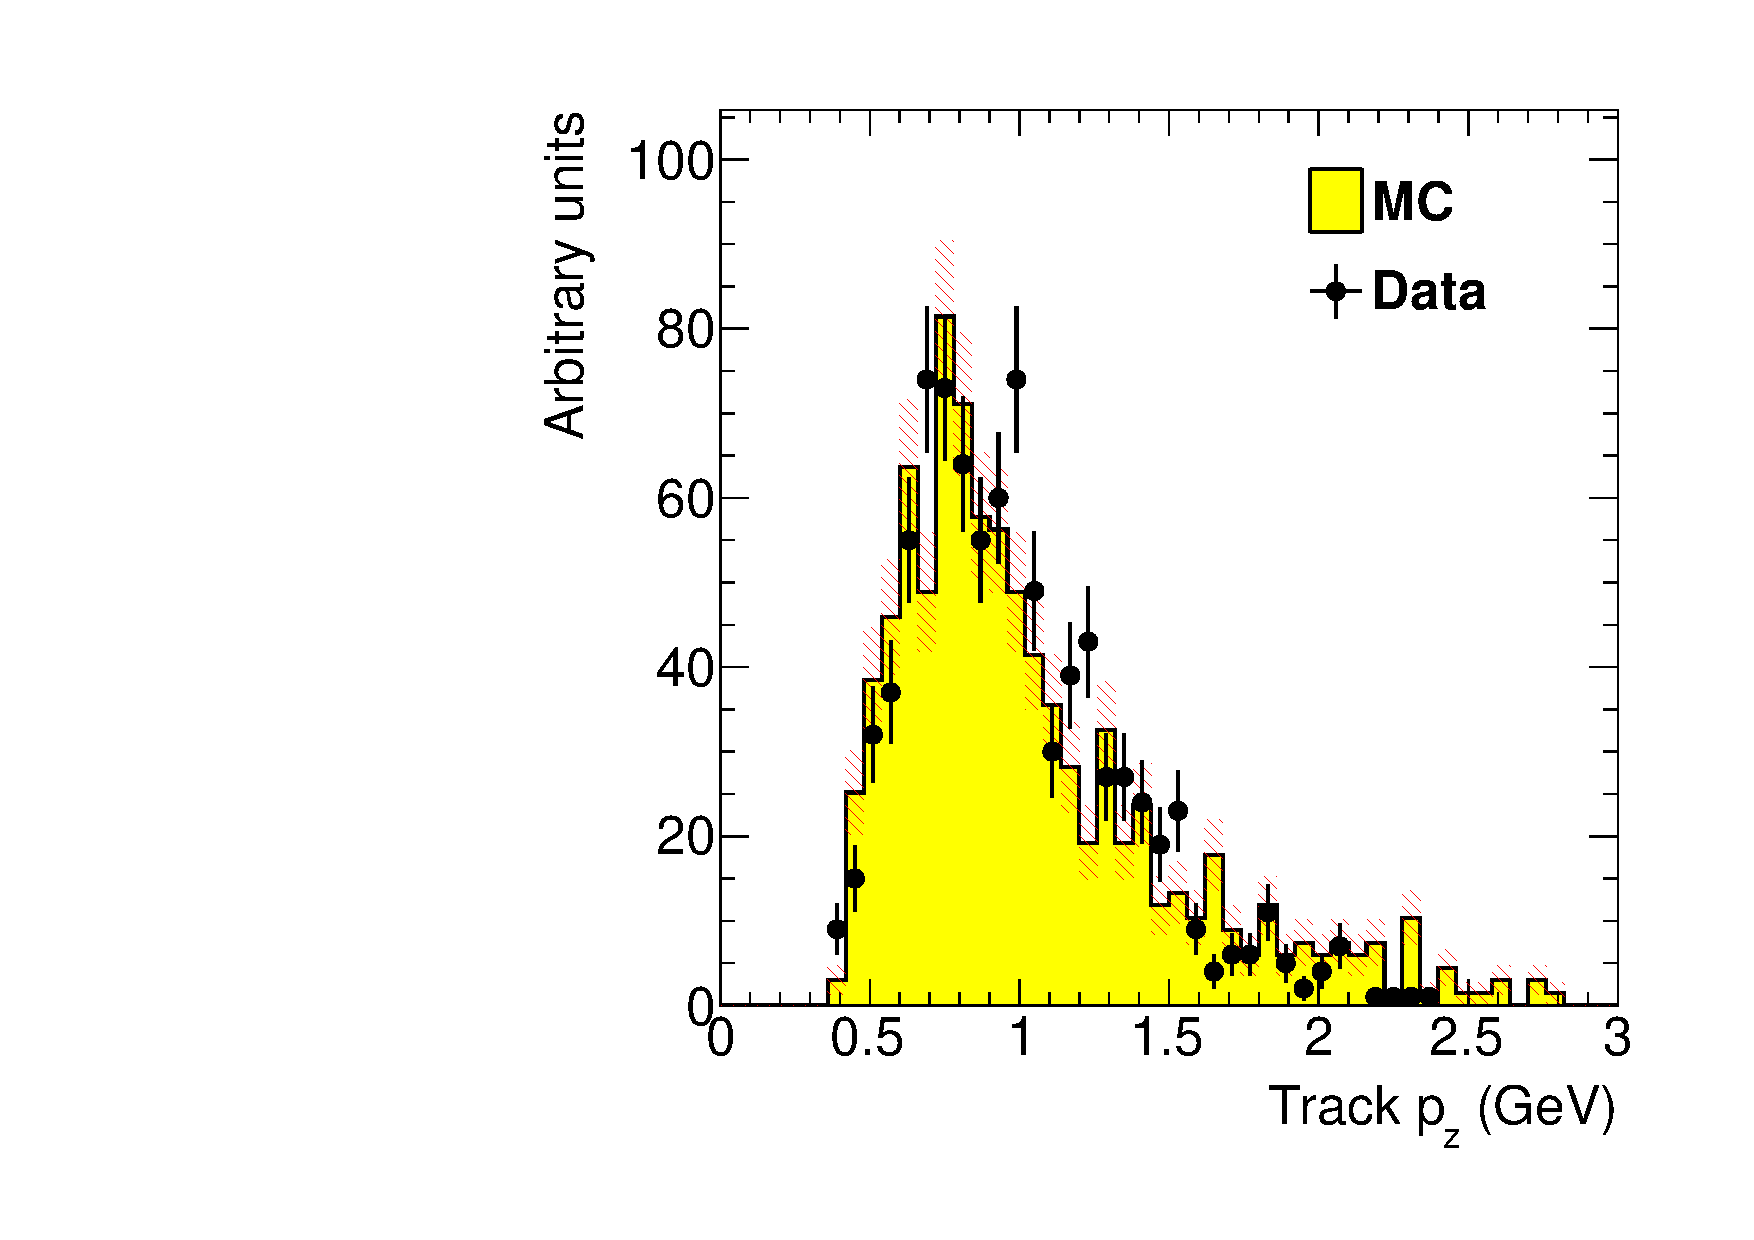
\includegraphics[width=5cm]{figures/h_trk_top_px_h_trk_top_px_trigsel4hit_pair1351_twotrkfilt-v6-paper}
   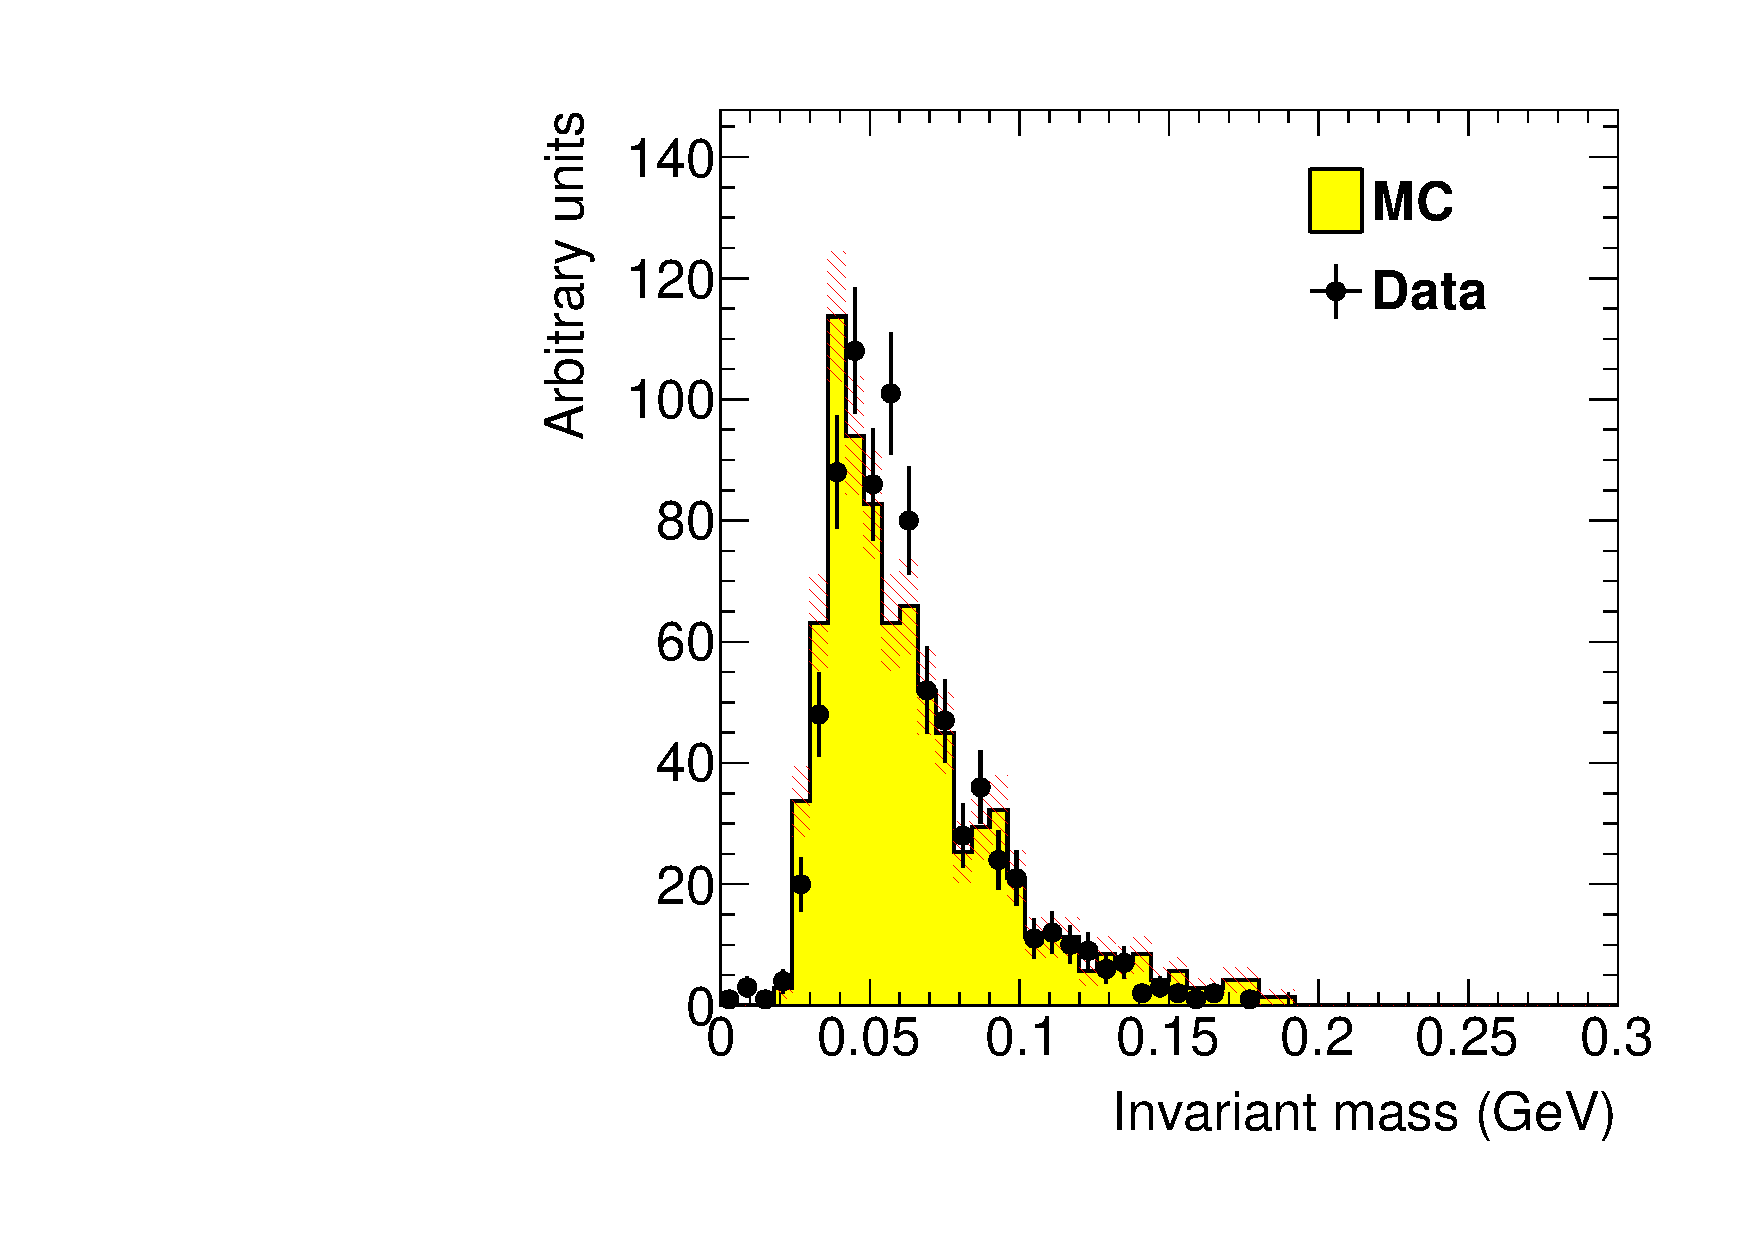
\includegraphics[width=5cm]{figures/h_invM_h_invM_trigsel4hit_pair1351_twotrkfilt-v6-paper}
   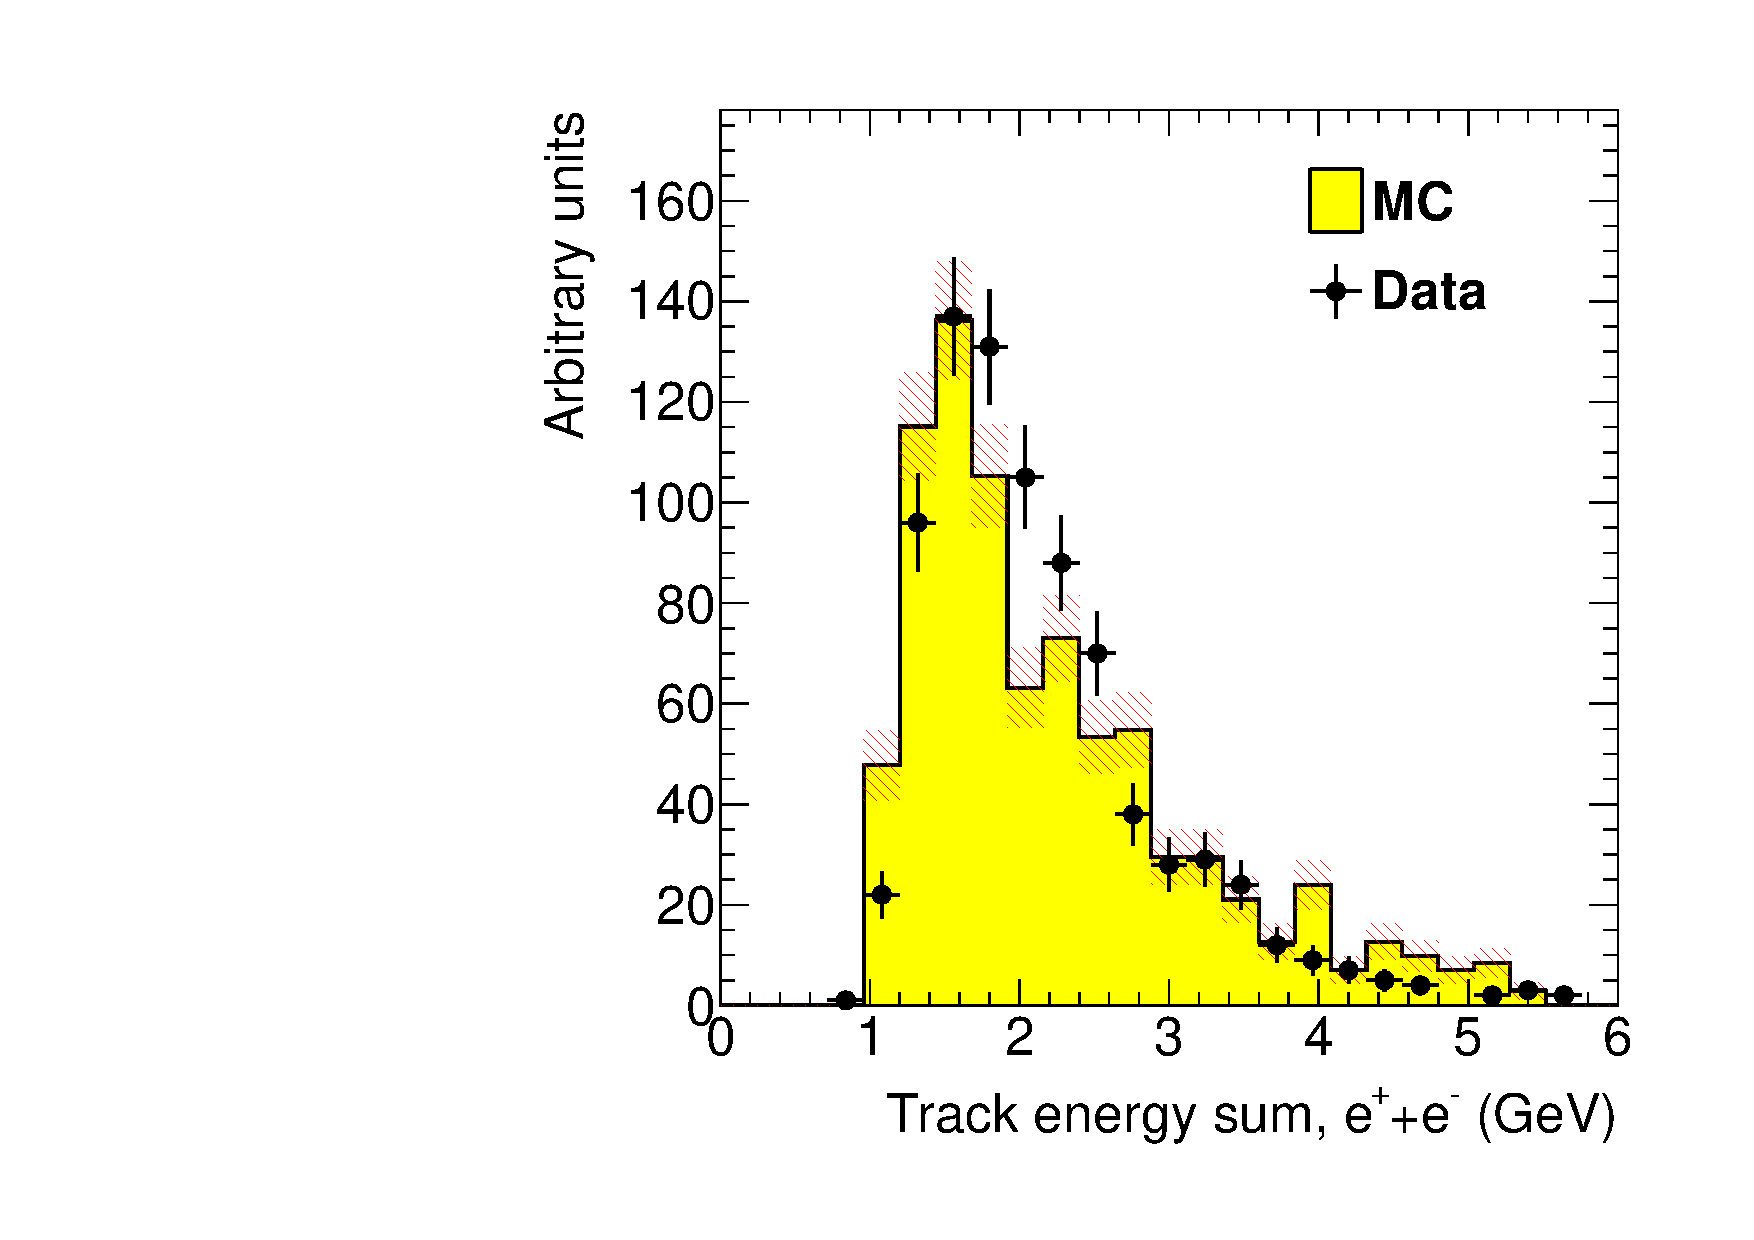
\includegraphics[width=5cm]{figures/h_sumE_h_sumE_trigsel4hit_pair1351_twotrkfilt-v6-paper}
\caption{Kinematic distributions for e$^+$e$^-$ pairs selected by opposite charged tracks in the top and bottom half of the tracker: track momentum in the top half of the SVT (left), invariant mass (middle) and the sum of the track momentum for the pair (right).}
\label{fig:pair_kin}
\end{figure*}
}
\end{center}
In the Test run, as well as in electron running with HPS, the dominant source of uncertainty in the 
tracking and vertexing is multiple Coulomb scattering. For the vertexing performance the foremost 
difference compared to electron beam running is that the target was located approximately 67~cm 
upstream from our nominal target position; giving almost collinear tracks in the detector. The increased 
lever arm over which tracks are extrapolated widens the resolution with up to a factor of eight (depending 
on momentum) compared to what is achieved at the nominal electron target position for HPS. 
Figure~\ref{fig:impact_param} shows the horizontal and vertical positions of the extrapolated track at the 
converter position. 
{\small
	 \begin{figure}[]
 \begin{center}
	% Plot info:
	% TestRun-v6 geometry, twotrkfilter, trigsel, hps-java-1.8-SNAPSHOT, 4hits, chi2<10
	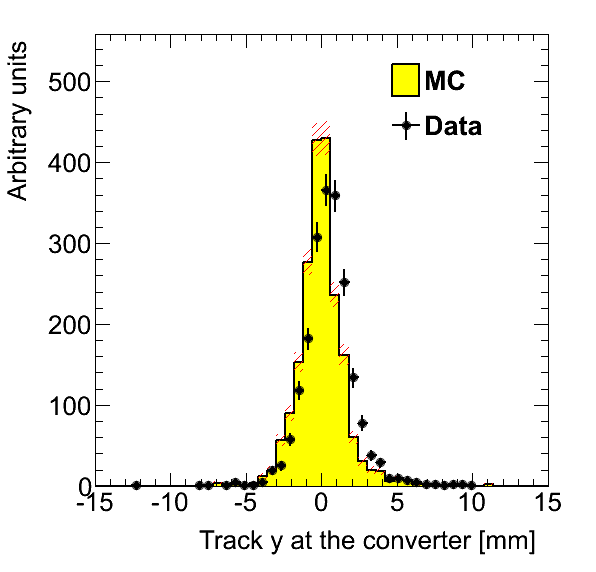
\includegraphics[width=7cm]{figures/h_trk_top_fr_conv_z_h_trk_top_conv_z_dataMC_twotrksel.png}
	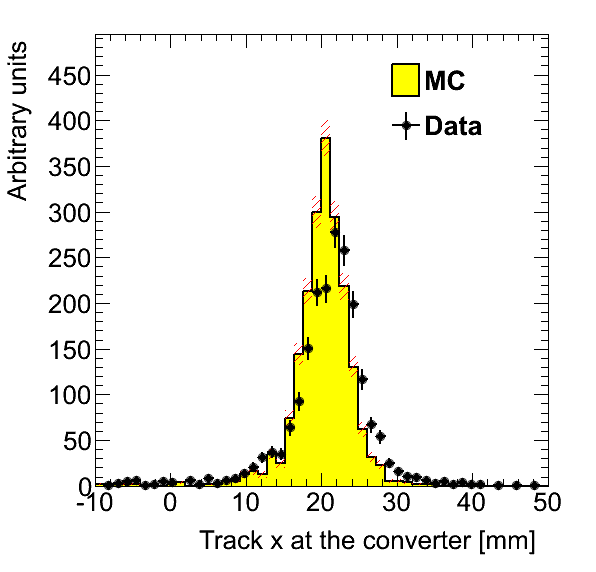
\includegraphics[width=7cm]{figures/h_trk_top_fr_conv_y_h_trk_top_conv_y_dataMC_twotrksel.png}
	\caption{ Vertical (top) and horizontal (bottom) extrapolated track position at the converter position 
	taking into account the measured fringe field. }
	\label{fig:impact_param}
\end{center}
\end{figure}
}
While residual alignment show small shifts good agreement on the widths between data and simulated 
events, indicating a good understanding of our material budget and distribution in the SVT.  Having 
the dominant contribution to the vertex resolution approximately right demonstrates that the resolution 
in HPS, with a target at 10~cm, will be as calculated.
%Furthermore, tails of the vertex distributions are impossible to study with the finite data sample obtained 
%in the Test run. Nevertheless, useful information can still be 
%obtained by studying the vertex distributions. Figure~\ref{fig:vtx_pos} shows the distance of closest 
%approach of the momentum vectors extrapolated in the upstream direction from our analyzing magnet, 
%taking into account the measured fringe field of the PS dipole magnet. 
 %\begin{center}
%{\small
%	 \begin{figure*}[t]
%	% Plot info:
%	% TestRun-v6 geometry, twotrkfilter, trigsel, hps-java-1.8-SNAPSHOT, 4hits, chi2<10
%	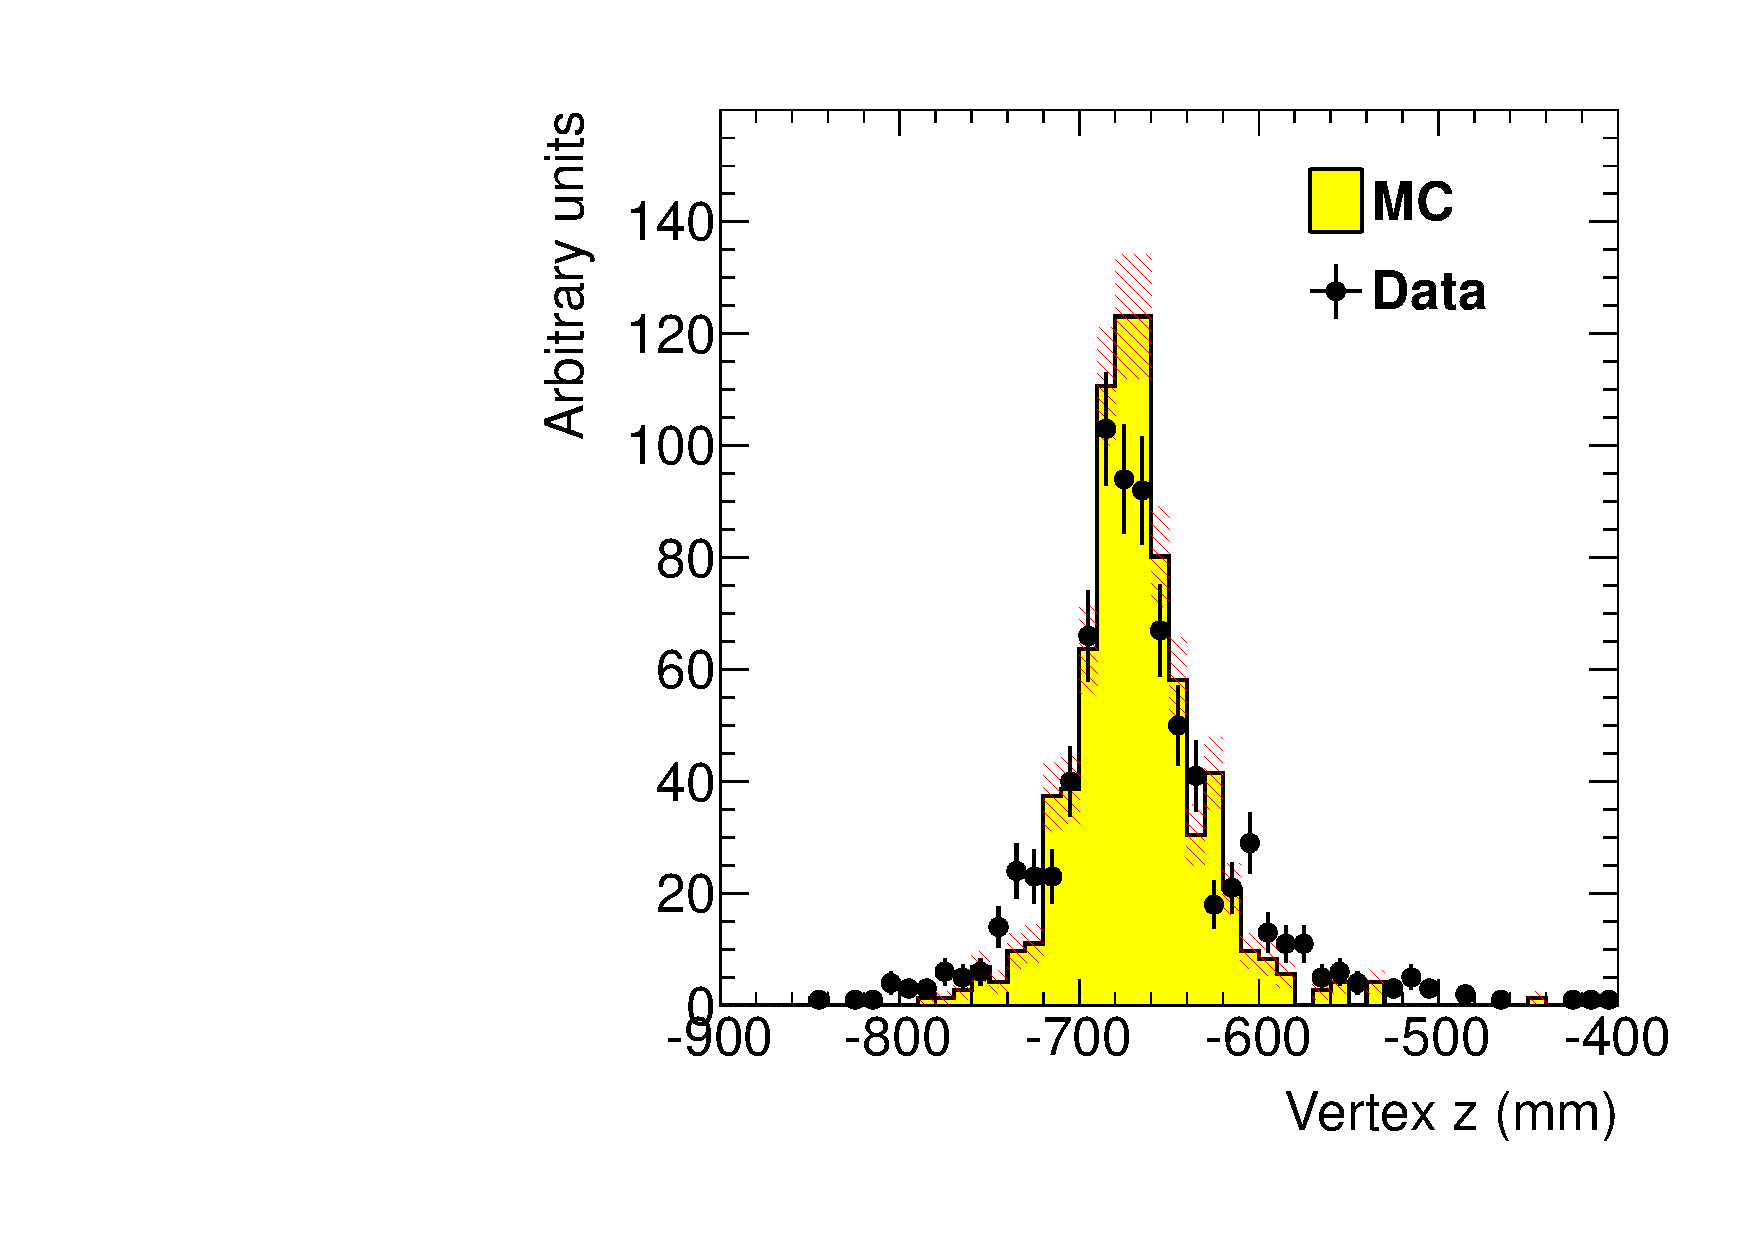
\includegraphics[width=5cm]{figures/h_vtx_fr_x_h_vtx_x_trigsel4hit_pair1351_twotrkfilt-v6-paper}
%	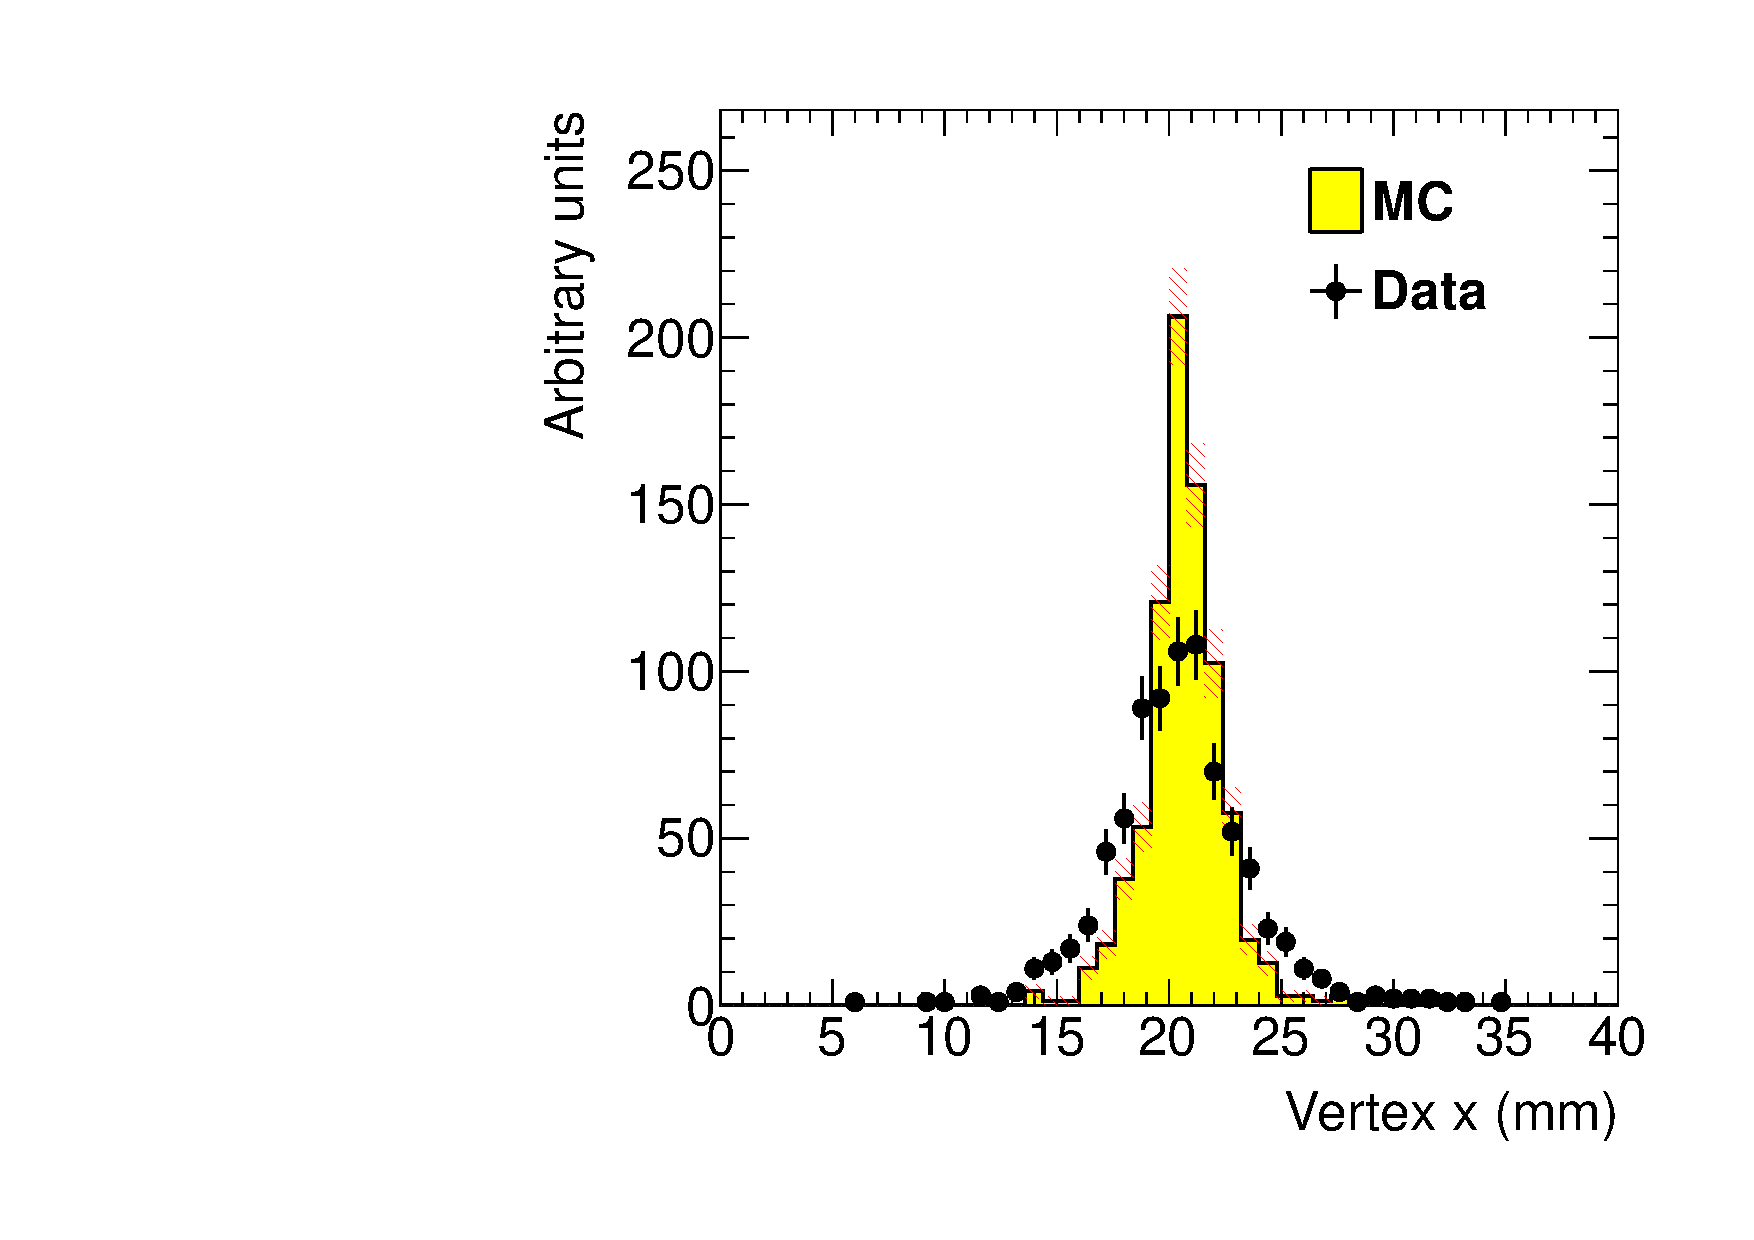
\includegraphics[width=5cm]{figures/h_vtx_fr_y_h_vtx_y_trigsel4hit_pair1351_twotrkfilt-v6-paper}
%	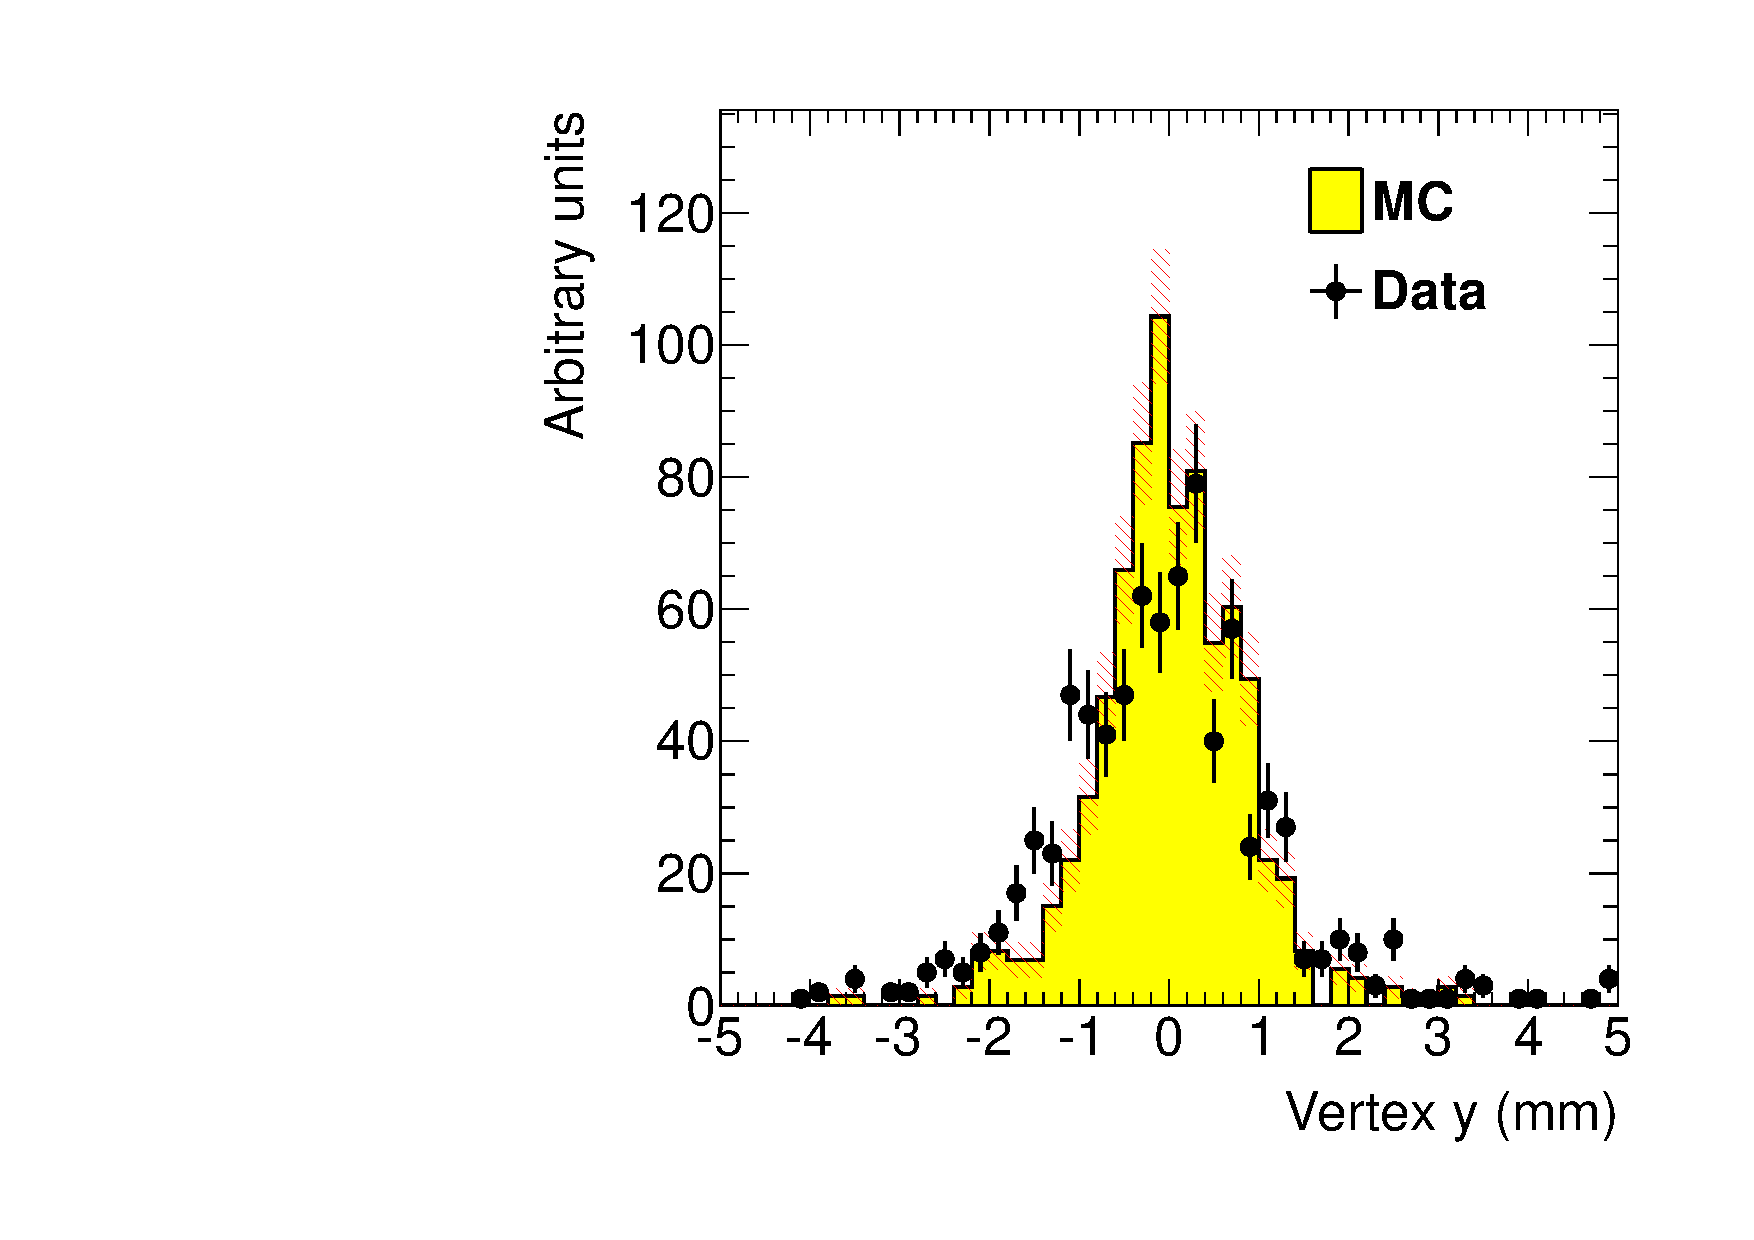
\includegraphics[width=5cm]{figures/h_vtx_fr_z_h_vtx_z_trigsel4hit_pair1351_twotrkfilt-v6-paper}
%	\caption{ Vertex position represented by the distance of closest approach of the extrapolated 
%	momentum vectors upstream of the PS dipole magnet taking into account the measured fringe field. 
%	The overall shift from zero in the x-direction is due to a 30~mrad rotation of the SVT with respect to 
%	the beam line.}
%	\label{fig:vtx_pos}
%\end{figure*}
%}
%\end{center}



\subsection{ECal Performance}
\label{sec:ecal_calibration}

The integrated pulse of each FADC channel was converted to energy by  
subtracting a pedestal and apply a conversion factor to convert ADC counts to energy. 
The pedestals are measured using special runs where each trigger records 100 samples of signals 
from the APDs with 4~ns between each sample. The pedestals were extracted from the 
part of the window before the actual hit in the calorimeter. Modules with signal above the threshold  
are clustered using a simple algorithm similar to the one 
deployed for the trigger (see Sec.~\ref{sec:trigger}). Due to the high effective readout threshold of 
73~MeV the average number of crystals in a cluster was $\sim 3$ and the simple clustering 
algorithm worked well for reconstruction of the detected shower energy. An average noise level of 
approximately 15~MeV was measured in special pedestal runs. 


The ratio of the ECal cluster energy $E$ to the momentum $p$ of a matched track in the SVT was used 
to determine the conversion factors from ADC counts to energy. To compare data and simulation, all 
inoperable or noisy channels in the SVT and ECal was disabled in both data and simulation so that any 
efficiency or bias that affect the data should be reflected in the simulation. 
%Furthermore, a conversion factor calibration is performed to equalize the gains of  each channel. 
%simulation to those observed in data by comparing .  The ``weighted $E/p$'' for each crystal is %computed, 
%representing the average $E/p$ for clusters that include the crystal
% $\frac{\sum_j w_{j,i}}{\sum_j\frac{P_j}{E_j}w_{j,i}}$.
Iteratively, conversion coefficients for each crystal is adjusted until the $E$/$p$ ratio in data and 
simulation are similar. The distribution of the $E$/$p$ ratio in data and simulation are compared in 
Fig.~\ref{fig:gains}. 
{\small
\begin{figure}[]
\begin{center}
	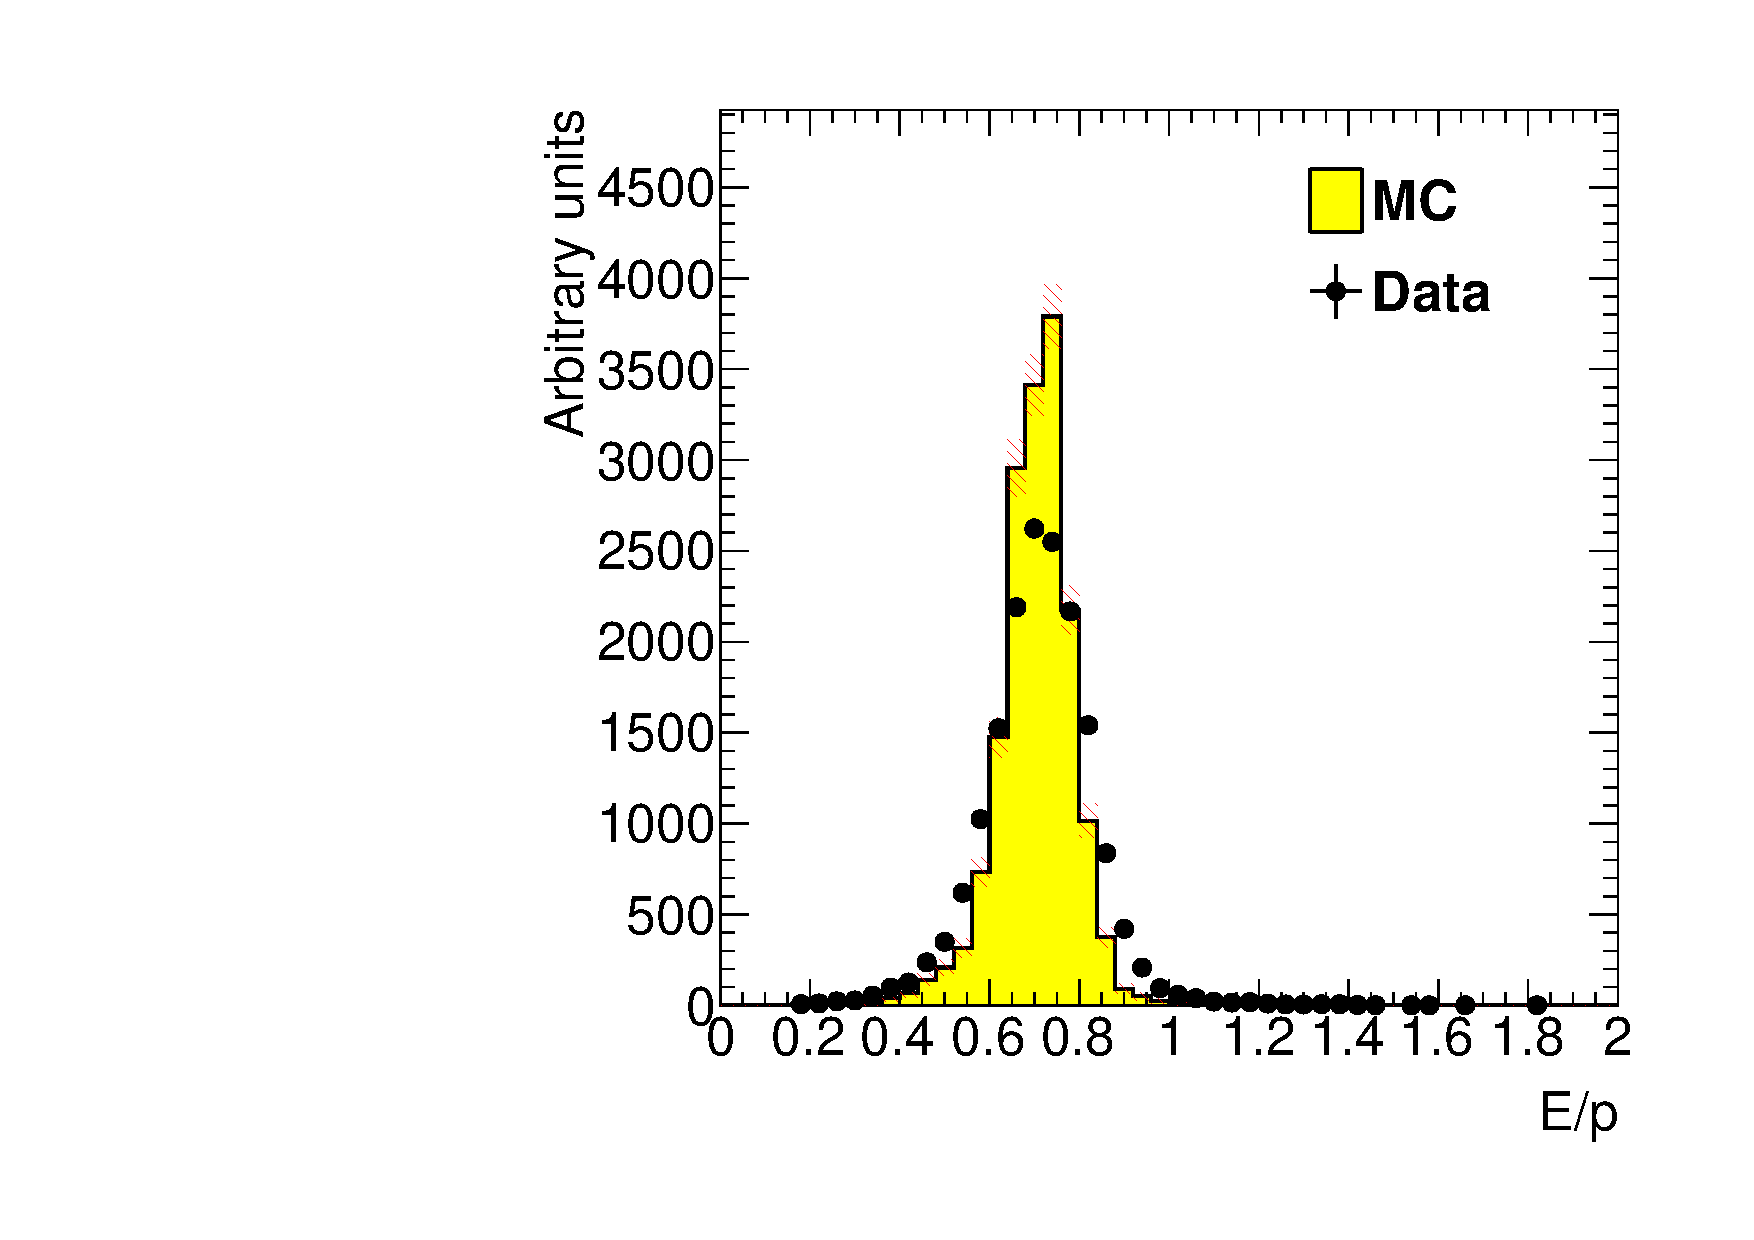
\includegraphics[width=7cm]{figures/h_ep_data_0_h_ep_MC_0_dataMC_1351-v6-v6gains_2-trig-top-cl600reg0.pdf}
	\caption{The ECal energy over track momentum ratio ($E$/$p$) comparing data and simulation 
	for inclusive events in the top half of the ECal.} 
	\label{fig:gains}
\end{center}
\end{figure}
}
The peak position of the distribution indicates the sampling fraction of the ECal, the fraction of the 
incident particle energy measured in the cluster. The width and tails of the distribution 
in data indicates imperfect calibration and noise of the ECal modules. This level of calibration and the 
agreement with simulation was found to be sufficient to study normalized event rates on the Test run.




\subsection{Trigger Performance}
As described above the energy from each 
crystal is measured differently in the trigger and what is readout from the ECal. 
The trigger performance was studied by simulating the 
trigger for each event and comparing to how the events were actually triggered.
To eliminate trigger bias, we use a tag and probe method: to study the trigger performance in one half 
of the ECal, we select 
events which triggered the other half and where there was exactly one probe cluster in the ECal half 
under study. We then measure trigger efficiency as the fraction of tagged events that fired the trigger in 
the probe half as a function of the probe cluster energy, shown in Fig.~\ref{fig:turnon}. 
\begin{figure}[ht]
\begin{center}
{\small
	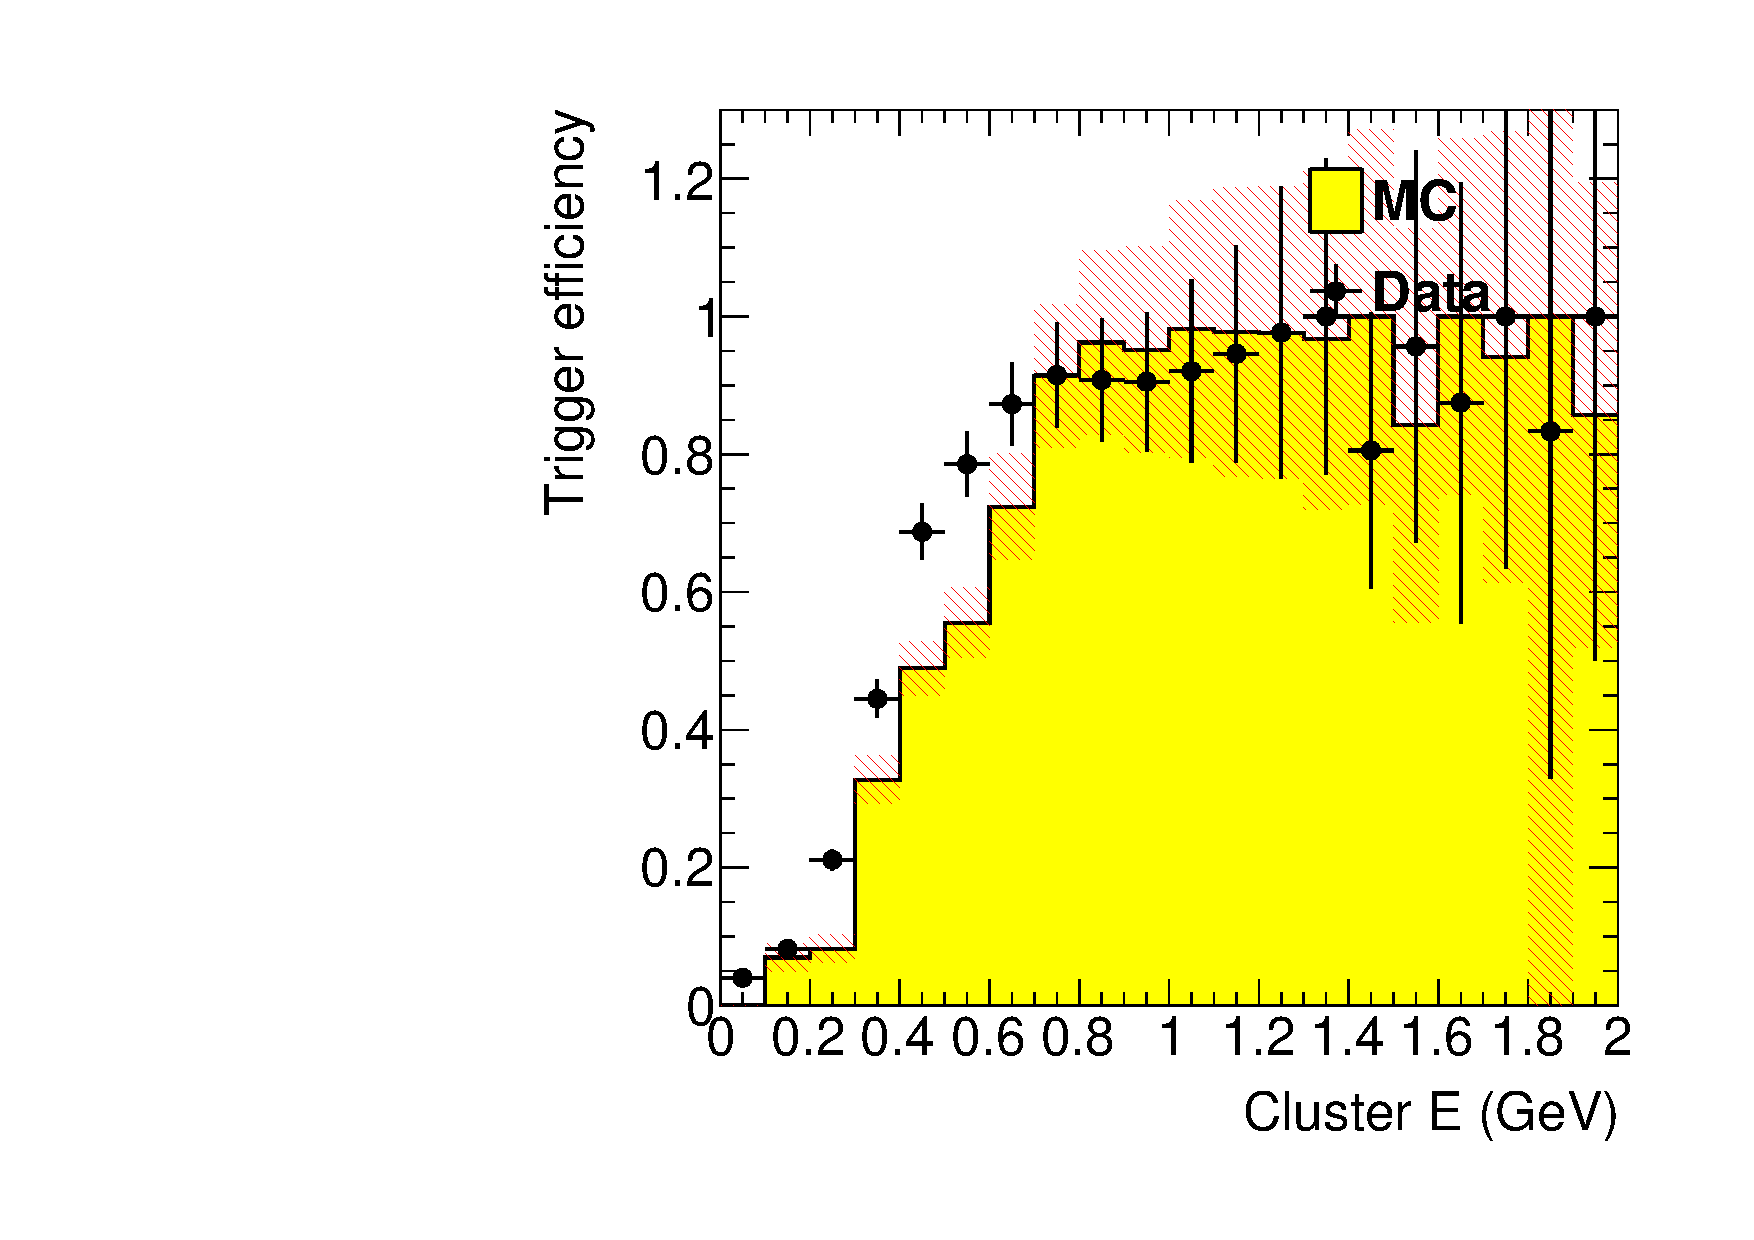
\includegraphics[width=7cm]{figures/h_cl_E_probedata_eff_h_cl_E_probeMC_eff_dataMC_1351-v7-trig-tagBot.pdf}
	\caption{Trigger efficiency in both halves of the ECal for data and simulation as a 
	function of cluster energy.}
\label{fig:turnon}
}
\end{center}
\end{figure}
The trigger turn-on is slow and reaches an uneven plateau just below 1~GeV for two reasons;  
gain variations between different crystals lead to the threshold variations and the nonlinearity of 
the time-over-threshold integral means that the effective threshold is higher for clusters that span 
multiple crystals. The effective trigger threshold is therefore dependent on position and energy of 
the particle as well as cluster multiplicity. 

As a cross-check we simulate the FADC trigger path by converting from readout hits (with fixed-size 
window integration) to trigger hits (time-over-threshold integration). The CTP clustering 
algorithm and the trigger decision from the SSP is simulated before we compare the trigger decision 
and trigger time to what was reported by the actual trigger. For every event, the trigger reports the 
trigger decision as a bit mask (top half, bottom half or both) and the time the trigger fired.
The turn-on from the trigger threshold was measured to be 1280 in units of ADC counts as expected. 
The threshold was not perfectly sharp because of uncertainties in the conversion from readout to trigger 
hits described above, but based on comparisons with simulation we found that the 
trigger worked exactly as specified.


\subsection{Trigger Rate Comparisons}
\label{sec:mcs}
Trigger rates observed in the Test run are dominated by multiple Coulomb scattered \ee pairs in the 
converter. In simulated events, the rate of triggers depend on the modeling of the pairs angular 
distribution and the subsequent multiple Coulomb scattering in the converter. Rates from different 
converter 
thicknesses are used to study the varying multiple Coulomb scattering contribution (pair production 
angle is constant). Restricting clusters to a well calibrated region of the ECal and subtracting the 
"no converter" background we see agreement with the rates predicted by the \egs{} simulation 
program, see Tab.~\ref{tab:mcs}.
%\begin{center}
\begin{table}
{\small
\begin{tabular}{|l|c|c|c|}
\hline
\bf Converter (\%~$X_0$) & \bf 1.60 & \bf 0.45 &	\bf 0.18 \\
\hline
EGS5 &	1162 $\pm$ 112 &	255 $\pm$ 28 &	94 $\pm$ 17	\\
\hline
GEANT4 & 2633 $\pm$ 250 & 	371 $\pm$ 38 &	114 $\pm$ 18 \\
\hline
Observed 	& 1064 $\pm$ 2 & 196 $\pm$ 1 &	92 $\pm$ 1 \\						
\hline
\end{tabular}
\caption{ Observed and predicted number of events for 1~s of beam at 90~nA for three different converter 
thicknesses. The uncertainty on the prediction includes systematic uncertainties from ECal alignment, background normalization, beam current normalization and limited statistics in the simulation.}
}
\label{tab:mcs}
\end{table}
%\end{center}
This gives further confidence that the dominant source of background occupancy for HPS, multiple 
Coulomb scattered beam electrons, is well 
described~\cite{Attwood:2005zz,Shen:1978ha,Gottschalk1993467} . 
%One of the main goals of the Test run was to evaluate the description of the tails of the 
%multiple Coulomb scattering to gain further confidence in the expected detector occupancy in the full HPS 
%experiment. Those occupancies have been evaluated using \egs{}~\cite{egs5} simulation program 
%whose \moliere{} formulation of multiple scattering show good agreement with previous studies 
%for a wide range of materials and projectiles~\cite{Attwood:2005zz,Shen:1978ha,Gottschalk1993467}. 
%Despite all data taken with a photon beam in the Test run, 






%%%%%%%%%%%%%%%%%%%%%%%%%%%%%%%%%%%%%%%%%%%%%%%%%%


%\section{Multiple Coulomb Scattering Distributions}
%\label{sec:mcs}
%Occupancies close to the beam create many of the key challenges in the HPS experiment
%and determine the limits of sensitivity to low \Aprime{} masses.
%These occupancies are dominated by electrons which have multiple Coulomb scattered (MCS) 
%to relatively large angles in the target. Because HPS is sensitive to scattering angles far out on the tail of 
%the MCS distribution, well beyond the angles important in other experiments, care must be taken
%to ensure our simulations are correct in this regime.  
%
%\subsection{Multiple Coulomb Scattering Models}
%
%One of the main goals of the HPS Test was to evaluate the description of the tails of the MCS
%to gain further confidence in the expected detector occupancy in the full HPS experiment. 
%Previous studies of multiple scattering angles show good agreement with the \moliere{} 
%theory~\cite{Moliere:1948zz} for a wide range 
%of materials and projectiles~\cite{Attwood:2005zz,Shen:1978ha,Gottschalk1993467}. We have verified 
%that the angular distribution $F(\theta)$ in the differential cross section 
%$d\sigma = F( \theta) d(\cos\theta) d\phi$ for the \egs{}~\cite{egs5} simulation program show good 
%agreement with \moliere{}'s analytical formula as formulated by Bethe~\cite{Bethe:1953va}. 
%The small angle approximation was also shown to be in agreement with the theory formulated by 
%Gaudsmit and Saunderson~\cite{Goudsmit:1940zza,Goudsmit:1940zz} that is valid for any angle. 
%While \egs{} uses the more complex and time consuming \moliere{} 
%formula, the default physics list of \geant{} uses the so-called Urban model, an approximation with two, 
%continuously joined, functions to take into account 
%small and large angle scattering. Due to the explicit function in large angle approximation used by 
%\geant{} we expect that \geant{} will overestimate the angular distribution at angles larger than a few 
%mrad.
%
%
%Figure~\ref{fig:schematic_testrun_vs_erun} gives a schematic view of the main differences 
%between the photon and electron beam setup. 
%The angular distribution of the pair produced electron and positron emerging 
%from the converter in the test run has comparable contributions from {\it i)} the pair production angle
%and {\it ii)} the MCS of the electron and positron in the converter after production. By measuring the 
%scattering rate at several different converter thicknesses we can vary the contribution from MCS 
%while the contribution from the pair production angle is constant. This allows us to confirm our model of MCS 
%despite the fact that all data was taken with a photon beam.
%
%
%\subsection{Running Conditions}
%
%Data was taken at three different converter thicknesses with a beam current varying between 
%$30-70$~nA, see~Tab.~\ref{tab:currents}.  
%\begin{table}[t]
%\begin{center}
%{\small
%\begin{tabular}{|c|c|c|}
%\hline
%Converter thickness & Duration &  $e^-$ on converter \\
% (\%$X_0$) & (s) & ($\mu$C)    \\   
%\hline
%%\hline
%1.6   & 911 &   24.4 \\ %24385.9     \\ %27 nA
%%\hline
%0.18   & 2640 &   193.5 \\ % 193508.9  \\  %73 nA
%%\hline
%0.45  & 2149 &     140.7 \\ %  140709.9  \\ %65.5 nA
%%\hline
%0    & 1279  &   88.1 \\ %88079.6  \\
%\hline
%\end{tabular}
%}
%\caption{Measured integrated currents for the dedicated photon runs.}
%\label{tab:currents}
%\end{center}
%\end{table}
%The photon beam line during the test run produced a relatively 
%large fraction of pairs 
%originating upstream of the converter. This contribution was measured during data taking 
%with ``empty'' converter runs i.e. removing the converter but with all other conditions 
%the same. 
%The upstream background measured in the ``empty'' converter runs was subtracted 
%from the other runs, properly normalized using the measured integrated currents.
%
%
%
%\subsection{Measured Angular Distributions}
%
%For this analysis, we measure angular distribution of electrons and positrons using the ECal.
%Cluster reconstruction was done using the algorithm described in Sec.~\ref{sec:trigger} build 
%clusters around seed hits (hits above a ``seed'' energy threshold and with greater energy than any 
%neighboring hits), and add all neighboring hits above an ``add'' energy threshold.
%Hit energy is calibrated by matching track momentum to cluster energy, as described in Sec.~\ref{sec:ecal_calibration}. The measured angular distribution in the ECal for the three converter thicknesses are shown in Fig.~\ref{fig:ang_distr_data}. 
%\begin{figure}[]
%\begin{center}
%{\small
%%	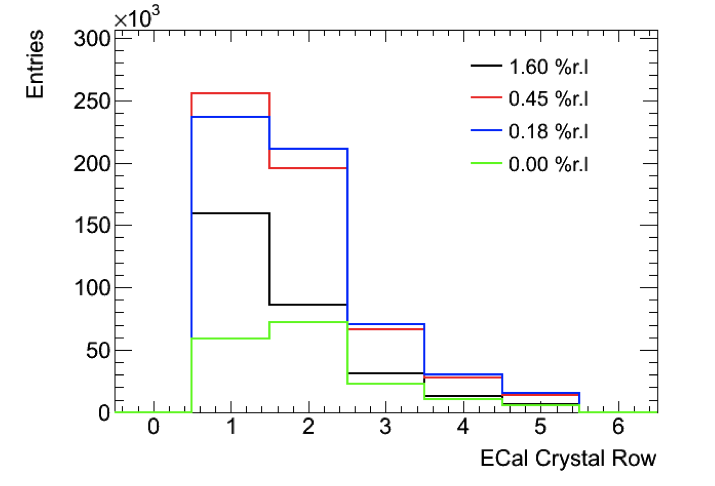
\includegraphics[ width=7cm]{figures/rate_ecalrow_raw.png}
%	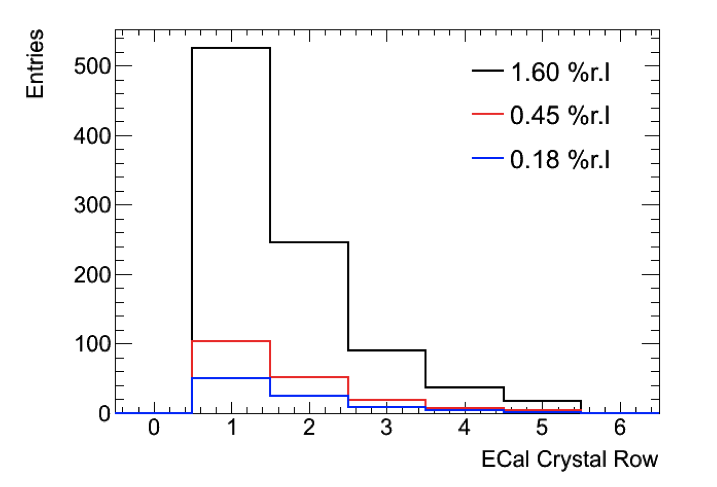
\includegraphics[ width=7cm]{figures/rate_ecalrow_norm_subtr.png}
%	\caption{Measured vertical angular distributions after integrated beam current 
%	normalization and background subtraction.}
%	\label{fig:ang_distr_data}
%}
%\end{center}
%\end{figure}
%The data has been normalized to the integrated beam current and the background has been 
%subtracted. The background fraction for the there converter thicknesses was 16\%, 52\% and 71\% 
%for converter thicknesses of 1.6\%, 0.45\% and 0.18\%, respectively. The background fraction was also 
%cross-checked by pointing back tracks reconstructed in the SVT to identify the fraction of tracks not emanating from the converter. 
%%This can be seen in Fig.~\ref{fig:extrapol_converter} (bottom) where small 
%%satellite peaks at $\pm 10$~mm can be identified as tracks from the upstream background. The angular distribution, after normalization and subtracting the upstream background, are shown in 
%%Fig.~\ref{fig:ang_distr_data} (right).  
%We also checked that the contribution from photons to our triggered 
%sample was less than 2\% (without angular selections which would further reduce the contribution).
%
%
%These measured angular distributions are compared to simulation to validate 
%the modeling of the MCS. \egs{}~\cite{egs5} is used to generate 
%the electromagnetic interactions in the converter while \geant{} is used to simulate the particles after the 
%converter.  Figure~\ref{fig:ang_distr_dataMC} shows the angular distribution comparing data and 
%\egs{} normalized to 1~s of beam at 90~nA beam current with a converter thickness of 1.6\%. 
%Reasonable agreement is obtained in the most important region close to the beam. There is a hint of a 
%slightly different slope of the data at larger angles; this difference is covered by systematic uncertainties.  
%The total rates for each converter thickness is shown in Fig.~\ref{fig:rate_vs_thickness} and summarized 
%in Tab.~\ref{tab:ang_distr_dataMC}.
%\begin{figure}[]
%{\small
%	\begin{center}
%	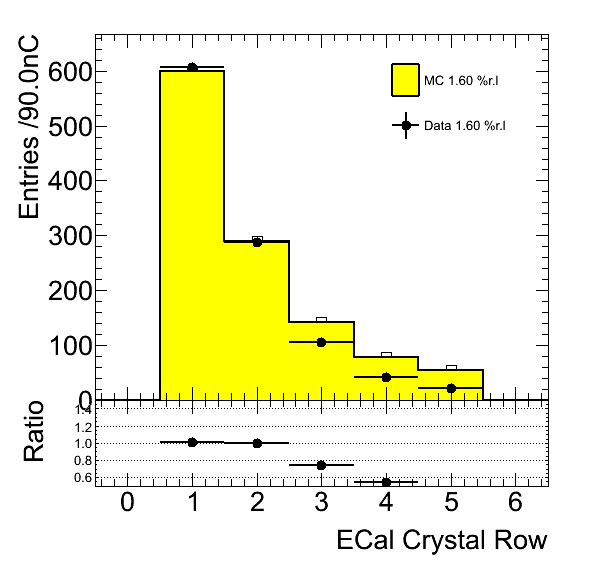
\includegraphics[ width=7cm]{figures/dataMC_1351_Hit_Y_top_norm_bkgsub.png}
%	\caption{Comparison between the observed and predicted angular distribution using \egs{} for a 
%	converter thickness of 1.6\%. Similar agreement is found for 0.45\% and 0.18\% converter thicknesses. 
%	Only statistical uncertainties are shown. }
%	\label{fig:ang_distr_dataMC}
%\end{center}
%}
%\end{figure}
%\begin{figure}[]
%\begin{center}
%{\small
%	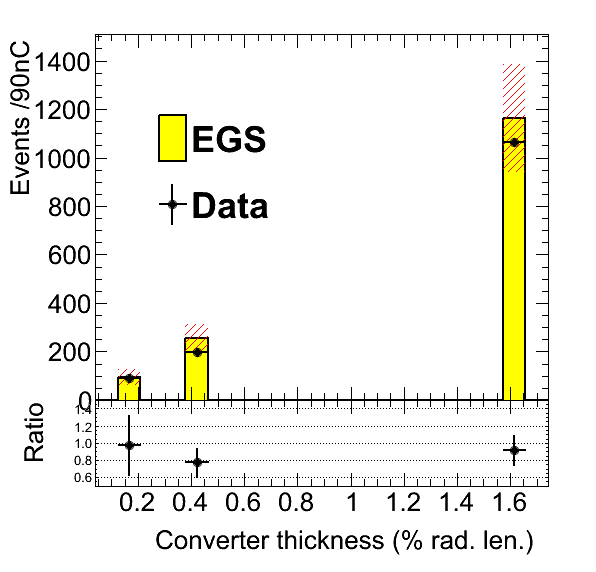
\includegraphics[ width=7cm]{figures/dataMC_egs.png}
%	\caption{The measured rate as a function of converter thickness for data and \egs{} simulation 
%	of MCS in 	the converter.} 
%	\label{fig:rate_vs_thickness}
%}
%\end{center}
%\end{figure}
%The total systematic uncertainty was estimated to be between 10-18\% depending on the run including:  
%a 5\% uncertainty on the integrated current normalization, alignment of the ECal, uncertainty from the 
%background normalization, and limited Monte Carlo statistics.  
%\begin{center}
%\begin{table}
%{\small
%\begin{tabular}{|l|c|c|c|}
%\hline
%Converter (\% r.l.) & 1.60 & 0.45 &	0.18 \\
%\hline
%EGS5 &	1162 $\pm$ 112 &	255 $\pm$ 28 &	94 $\pm$ 17	\\
%\hline
%GEANT4 & 2633 $\pm$ 250 & 	371 $\pm$ 38 &	114 $\pm$ 18 \\
%\hline
%Observed 	& 1064 $\pm$ 2 & 196 $\pm$ 1 &	92 $\pm$ 1 \\						
%\hline
%\end{tabular}
%\caption{ Observed and predicted number of events for 1~s of beam at 90~nA for three different converter 
%thicknesses. The uncertainty on the prediction includes systematic uncertainties. }
%}
%\label{tab:ang_distr_dataMC}
%\end{table}
%\end{center}
%
%\subsection{Conclusion}
%In summary, the accurate modeling of the MCS is fundamental to estimate occupancies and trigger rates 
%for HPS. \egs{} predicts the correct angular distribution across all converter thicknesses as expected while 
%\geant{}, using the so-called Urban model for multiple scattering overestimates the rates; with the disagreement 
%increasing  with larger converter thickness. This preliminary result verifies similar studies [] and gives confidence 
%in our modeling of the MCS 
%using \egs{} for evaluating the physics reach of HPS.




%%%%%%%%%%%%%%%%%%%%%%%%%%%%%%%%%%%%%%%%%%%%%%%%%%


\section{Summary and Outlook}
The HPS Test experiment, using a simplified version of the apparatus planned for the full HPS 
experiment in a parasitic photon beam, demonstrated the feasibility of the detector technologies 
proposed for the silicon vertex tracker, electromagnetic calorimeter, and data acquisition systems. 
Performance from each of these subsystems has been shown to be adequate to conduct the full 
experiment successfully. Studies of multiple Coloumb scattering tails of electrons and positrons from 
photon conversions further backs expectations from simulation, giving credance to estimates of the 
detector backgrounds expected in electron beam running for HPS.  

%The test run achieved the following detector performance:\begin
%{enumerate}
%	\item More than 97\% of SVT channels functioned properly
%	\item Silicon detector signal to noise was 25.5, good enough %to achieve the expected resolutions
%	\item SVT hit time resolution was 2.6 ns, which will permit %background rejection with tight timing cuts 
%	\item SVT hit efficiency was greater than 98\%
%	%\item SVT track reconstruction efficiency was greater than %98\%
%	\item 87\% of ECal crystals functioned properly, with %%defects to be corrected by planned ECal upgrades
%	\item The ECal has been successfully calibrated using SVT %tracks
%	\item The SVT and JLab DAQ were successfully integrated
%	\item The trigger functioned as designed; the FADC trigger 
%rate was tested to greater than 100~kHz
% deficiencies found in test run trigger performance are 
%addressed for the 2014-2015 run
%\end{enumerate}

%While the Test Run successfully allowed us to test many aspects %of the HPS experiment, there were 
%limitations to what could be achieved in some key areas such as %mass resolution and vertexing 
%performance. In particular, the low statistics and lack of 
%resonances or scattered beam electrons prohibits a 
%direct analysis of the momentum 
%and tails of the vertex distribution. However, for both of these %performance parameters, the observed 
%agreement between data and simulation in key distributions 
%supports the performance expected for the 
%proposed experiment. 



%\subsection{Lessons Learned}

%In the process of developing the HPS Test design, it was found 
%that this simple system was capable of 
%delivering a surprising fraction of the physics potential 
%anticipated for the full experiment.  With this in mind, 
%we have proposed a new design for the HPS detector that builds 
%upon the HPS Test , principally 
%by addressing the compromises made for HPS Test to ensure the 
%best possible performance for A$^\prime$ 
%physics within the envelope of the existing beam line layout and %analyzing magnet. For the SVT, 
%this design uses the same sensors, readout chips, and module 
%concept and for the ECal the crystal and 
%detector layout will be identical, retaining the most successful 
%elements of the test run apparatus and addressing the weaknesses %identified during assembly and 
%operation to ensure the success of the 
%experiment. The new SVT layout restores the sixth layer for more %robust tracking, adds acceptance in the 
%deeper layers to increase sensitivity and provides better 
%silicon cooling to improve longevity. Other major 
%updates needed for the full experiment are updates to the SVT 
%electronics and 
%DAQ; improving connectivity and cabling, moving digitization 
%closer to the front-end electronics and 
%updating the data reduction, event handling and trigger 
%synchronization to reach 50kHz 
%trigger rates. 
%This first generation of 
%the full experiment will be ready to take physics data when 
%CEBAF begins operation again in 2014.


\section{Acknowledgements}
The authors are grateful for the support from Hall~B at JLab and especially Hall~B technicians 
for support during installation and decommissioning. They also would like to commend the CEBAF 
personnel for achieving good performance when we needed it; the last few hours of operating CEBAF6. 
The tremendous support from home institutions and supporting staff also needs praise from the authors. 

This work has been supported by the US Department of Energy. 


%% The Appendices part is started with the command \appendix;
%% appendix sections are then done as normal sections
%% \appendix

%% \section{}
%% \label{}

%% References
%%
%% Following citation commands can be used in the body text:
%% Usage of \cite is as follows:
%%   \cite{key}          ==>>  [#]
%%   \cite[chap. 2]{key} ==>>  [#, chap. 2]
%%   \citet{key}         ==>>  Author [#]

%% References with bibTeX database:

\bibliographystyle{model1-num-names}
%\bibliography{<your-bib-database>}
\bibliography{hps-testrun-nim}

%% Authors are advised to submit their bibtex database files. They are
%% requested to list a bibtex style file in the manuscript if they do
%% not want to use model1-num-names.bst.

%% References without bibTeX database:

% \begin{thebibliography}{00}

%% \bibitem must have the following form:
%%   \bibitem{key}...
%%

% \bibitem{}

% \end{thebibliography}


\end{document}

%%
%% End of file `elsarticle-template-1-num.tex'.
